% !TeX root = ../main.tex
% Add the above to each chapter to make compiling the PDF easier in some editors.

\chapter{Hyperparameter Optimization with Sparse Grids}\label{chapter:main_part}

\section{Methodology}

In the scope of this thesis, we implemented two new approaches for hyperparameter optimization. The first one is using sparse grids and the second one is based on the idea of random search. 

\subsection{Adaptive Grid Search with Sparse Grids}

The first new approach is using an adaptive sparse grid for the optimization. The idea is similar to conventional grid search because a grid is generated on the hyperparameter space and the machine learning model is evaluated with the configuration given by the grid points. However, there are major differences to the conventional grid search. The first one is the location and generation of the basis points. As described in Chapter \ref{chapter:theoretical_background}, sparse grids need fewer points to achieve similar accuracy for certain functions. Additionally, the grid is generated iteratively and can be adaptive to the underlying function. This adaptivity can be set with a specific parameter. For our implementation, we utilize the functionality given by the \textit{SG++} toolbox \cite{valentin2016hierarchical}. It allows to additionally interpolate the function given by the grid points with B-splines and apply several different kinds of optimization algorithms to find the best configuration.


\subsection{Iterative Adaptive Random Search}

Another new technique is based on the random search. For the optimization with the iterative adaptive random search, a fixed number of initial points are sampled in the hyperparameter space. In the following iterations, already existing points are refined meaning that points are sampled in the neighboring region. We implemented three different refinement strategies that determine, how points are refined. The main differences are the probability distribution and the intervals of the new search region. For this algorithm, we can also balance the trade-off between exploration and exploitation. A similar adaptivity parameter as introduced in the adaptive sparse grid search, is used to define which point is selected to be refined in each iteration step.

\subsection{Evaluation Metrics}

For this comparison, we used several kinds of artificial neural networks such as fully connected or convolutional ones. Additionally, multiple datasets of different sizes and with categorical or numerical features are being used. General tasks like for example regression with mean average percentage error as metric and object detection with accuracy as metric are optimized. To validate a hypothesis, more than one experiment with e.g. different data sets are used. 

\section{Sparse Grid Optimization of Functions}

\subsection{Implementation}
\label{subsec:Implementation}

The implementation was done in Python (version 3.10.6) and two main classes are introduced. The first is the \textit{Dataset} encapsulating the input and target data of the dataset used for the machine learning model. One can either instantiate an object with a given X and Y vector for the data and target or by giving a task id. This identification number is used to instantiate both arrays with the dataset that can be fetched with the functionality given by OpenML \cite{feurer-arxiv19a}. Each task has a unique id, we first concentrate on Regression tasks with small neural networks. \newline

The second class introduced is the Optimization class. The abstract super class has 5 concrete implementations, one for each of grid-, random search, bayesian optimization, the sparse grid search and iterative adaptive random search. In all cases, a dataset object has to be given. Additionally, the machine learning model as a function depending on the hyperparameters is required. For the sparse grid search, the functionality of the \textit{SG++} \cite{valentin2016hierarchical} is used. The function has to inherit the class \textit{ScalarFunction} and the concrete model evaluation is done in the member function \textit{eval(x)}. Also, the hyperparameter space has to be defined. This is a dictionary with information about the names and the types of parameters. Possible types are list for categorical ones, interval (int) for continuous (or integer) parameters, and log interval for ones that should be sampled logarithmically. Additionally, the lower and upper bound for each of them has to be provided. The next parameters are the budget defining the upper bound for function evaluations and the verbosity for outputs. \newline

For the sparse grid optimization, the hyperparameters have to be scaled to the standard interval $ [0,1] $ and back to the original one for interpretation. Therefore, the functions \textit{to\_standard}, \textit{from\_standard}, \textit{to\_standard\_log} and \textit{from\_standard\_log} are introduced for the linear and logarithmic scaling. 

\begin{lstlisting}[language=Python]
	def to_standard(lower, upper, value):
	return (value - lower) / (upper - lower)
	
	def from_standard(lower, upper, value):
	return value * (upper - lower) + lower
	
	def to_standard_log(lower, upper, value):
	a = math.log10(upper / lower)
	return math.log10(value / lower) / a	
	
	def from_standard_log(lower, upper, value):
	a = math.log10(upper / lower)
	return lower * 10 ** (a * value)
\end{lstlisting}

The parameters lower and upper are the bounds of the original hyperparameter interval. The value argument is then scaled to or from the standard domain $ [0,1] $, respectively. \newline 

Due to many stochastic influences in the scope of neural networks, reproducibility is not always given by default. Examples are the network's weight initialization, random dataset splitting, and shuffling during the training phase. To overcome this problem, the seeds of random functions can be set to be deterministic and reproducible.


\subsection{Test Functions}

Before optimizing the configurations of machine learning models, simple functions are used. This has the advantage that the optimal point is already known in advance and a function call is much faster than evaluating a neural network. Therefore, three different test functions are given with the following properties \cite{valentin2016hierarchical}:

\begin{table}[H]
	\caption{ Three test functions and their properties.}
	\label{tab:test_functions}
	\centering
	\begin{tabular}{|c c c c|} 
		\hline
		Function & Domain & $x_{opt}$ & $ f(x_{opt}) $\\
		\hline
		Eggholder & $[-512, 512]^2 $ & $(512, 404.2319)$ & $ -959.6407 $ \\
		Rosenbrock & $[-5, 10]^2 $ & $(1,1)$ & $ 0 $ \\
		Rastrigin & $[-2, 8]^d $ & $\vec{0}$ & $ 0 $ \\
		\hline
	\end{tabular}
\end{table}

The Eggholder function is defined with \cite{whitley1996evaluating} 
\begin{equation}
	f(x_0, x_1) = -x_0 * \text{sin}(\sqrt{ | x_0 - (x_1 + 47) | }) - (x_1 + 47) \text{sin}(\sqrt{ | x_1 +47 + \frac{x_0}{2} | }).
\end{equation}

The second function (Rosenbrock) \cite{yang2010engineering} is calculated with 
\begin{equation}
	f(x_0, x_1) = (1-x_0)^2 + 100 (x_1 - x_0^2)^2.
\end{equation} 
and the third one (Rastrigin) \cite{yang2010engineering} is defined with
\begin{equation}
	f(\vec{x}) = 10 d + \sum_{ i = 1 }^{d} (x_i^2 - 10 \text{cos}(2 \pi x_i))
\end{equation} 
where $ d $ is the dimensionality of the input vector $ \vec{x} $. Figure \ref{fig:test_functions_plot} shows the functions in two dimensions.


\begin{figure}[H]
	\begin{subfigure}{0.3\textwidth}
		\centering
		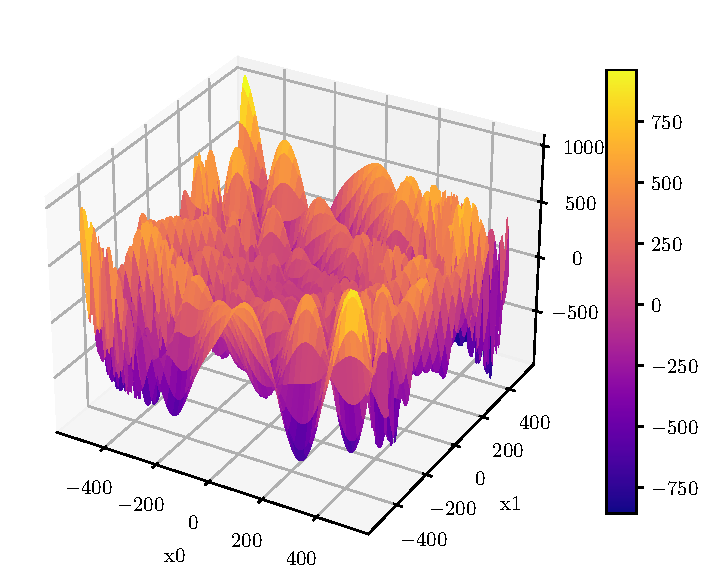
\includegraphics[width=\textwidth]{Eggholder_normal}
		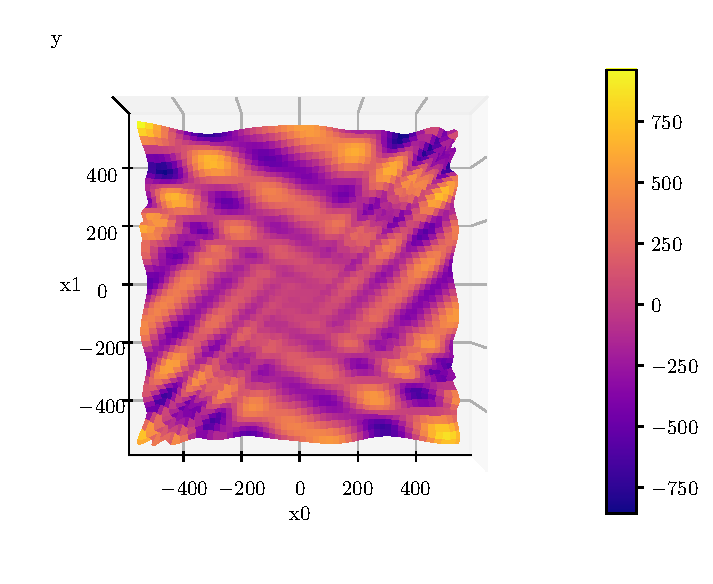
\includegraphics[width=\textwidth]{Eggholder_above}
		\caption{Eggholder.}
		\label{fig:Eggholder}
	\end{subfigure}
	\begin{subfigure}{0.3\textwidth}
		\centering
		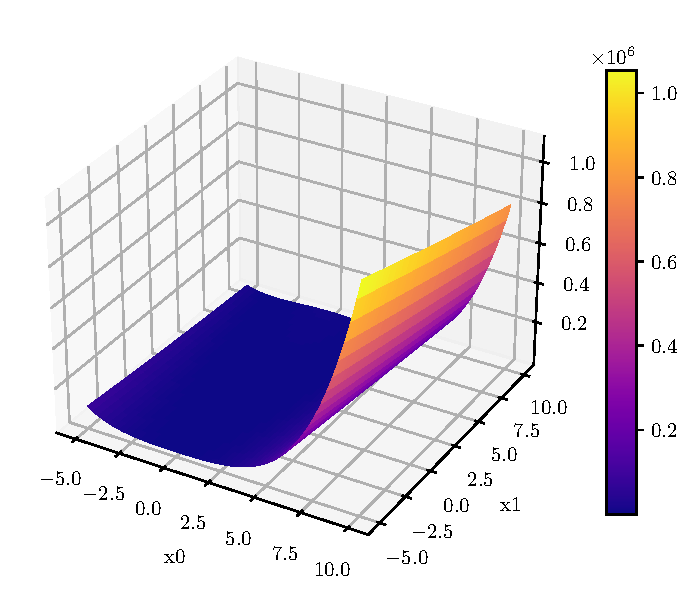
\includegraphics[width=\textwidth]{Rosenbrock_normal}
		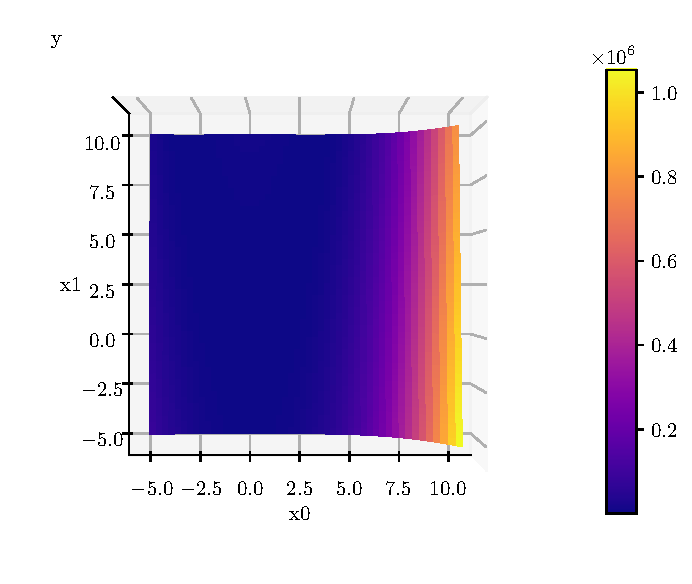
\includegraphics[width=\textwidth]{Rosenbrock_above}
		\caption{$ log_{10}(f) $ of Rosenbrock.}
		\label{fig:Rosenbrock}
	\end{subfigure}
	\begin{subfigure}{0.3\textwidth}
		\centering
		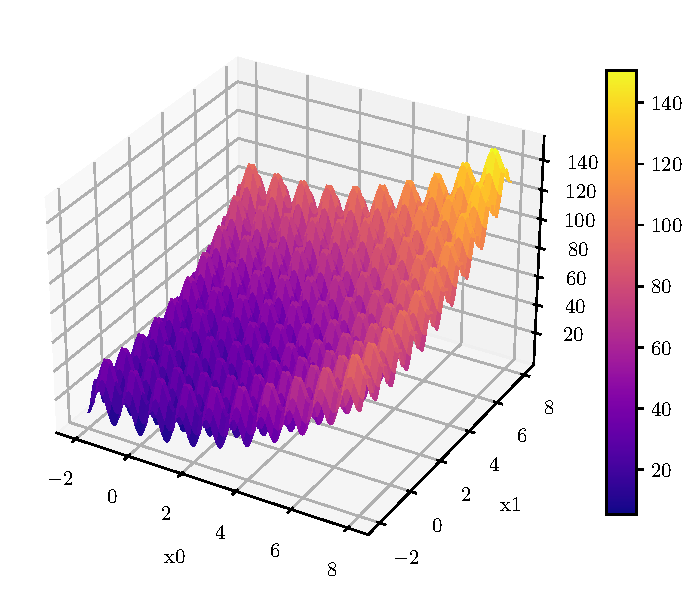
\includegraphics[width=\textwidth]{Rastrigin_normal}
		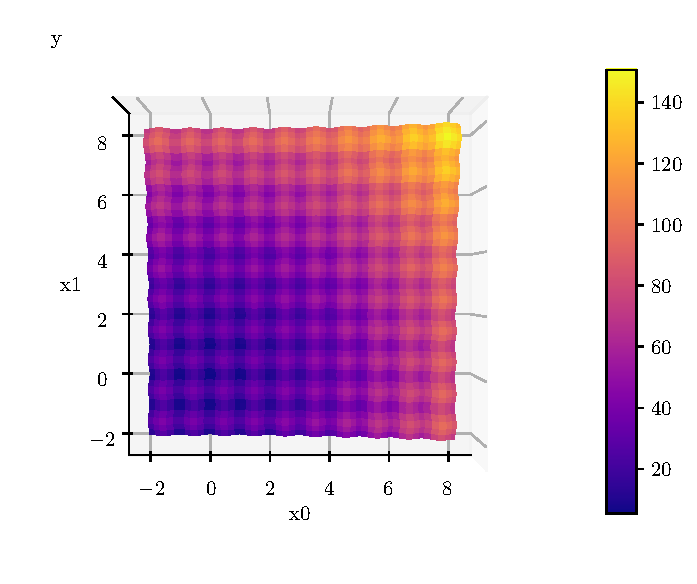
\includegraphics[width=\textwidth]{Rastrigin_above}
		\caption{Rastrigin.}
		\label{fig:Rastrigin}
	\end{subfigure}
	
	\caption{Test functions used for evaluating the sparse grid optimization. Each one is plotted with 200 samples in each dimension. Note that the function values of the Rosenbrock function are transformed with $ log_{10}(f(x)) $ for better visualization.}
	\label{fig:test_functions_plot}
\end{figure}

The Eggholder function (see Figure \ref{fig:Eggholder}) is oscillatory and the optimal point $ x_{opt} $ lays at the border of the domain. Additionally, it is multi-modal. The second one (see Figure \ref{fig:Rosenbrock}) is plotted with the function values additionally transformed with $ log_{10}(x) $ for better visualization. The last one is also multi-modal (see Figure \ref{fig:Rastrigin}). 

As a first step, the sparse grid generation which is done with the Ritter Novak refinement criterion \cite{b_splines} is evaluated. In each iteration, the grid point $ x_{l,i} $ that minimizes the product 
\begin{equation}
	(r_{l,i} +1)^{1 - \gamma} \cdot (||l||_1 + d_{l,i} + 1)^{\gamma}
\end{equation}
is refined. In this case, $ r_{l,i} = |\{ (l', i') \in K | f(x_{l',i'}) \le f(x_{l,i}) \}| \in \{1, ... , |K|\} $ is the rank of the grid point with $ K $ being the current set of level-index pairs of the grid. This rank denotes the place of the function value in the ascending order of all values of the current grid. On the other hand, the degree of the point $ d_{l,i} \in \mathbb{N}_0 $ is the number of previous refinements at this point. One important choice has to be made for the adaptivity parameter $ \gamma $. This value has to be between 0 and 1 and the smaller this value is, the more adaptive is the sparse grid. With this value, a trade-off between exploration and exploitation can be balanced. The optimal value generally depends on the function that has to be optimized. \newline

\subsection{Sparse Grid Generation with different Adaptivities}

In the following, the behavior of the sparse grid generation is analyzed with the help of the three test functions. In each case, 3 different values for the adaptivity parameter $ \gamma \in \{0.0, 0.5, 1.0\} $ are used and the resulting sparse grid with the triangulated function values is plotted. The first test case is the Eggholder function and the result is depicted in Figure \ref{fig:Eggholder_grid}.

\begin{figure}[H]
	\begin{subfigure}{0.3\textwidth}
		\centering
		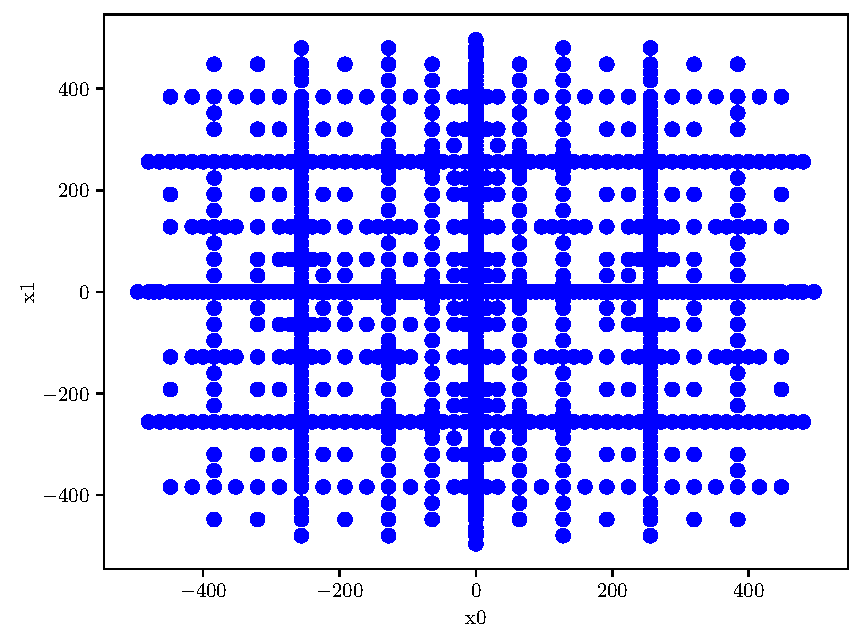
\includegraphics[width=\textwidth]{figures/Results/Sparse_grid_generation_results/Eggholder/tex_files/Eggholder_1}
		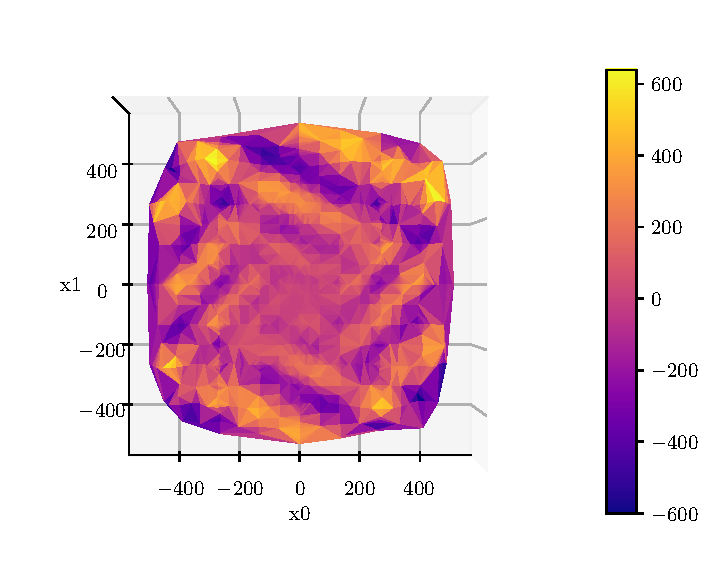
\includegraphics[width=\textwidth]{figures/Results/Sparse_grid_generation_results/Eggholder/tex_files/Eggholder_above_1}
		\caption{$ \gamma = 1.0 $}
		\label{fig:Egg_gamma_1}
	\end{subfigure}
	\begin{subfigure}{0.3\textwidth}
		\centering
		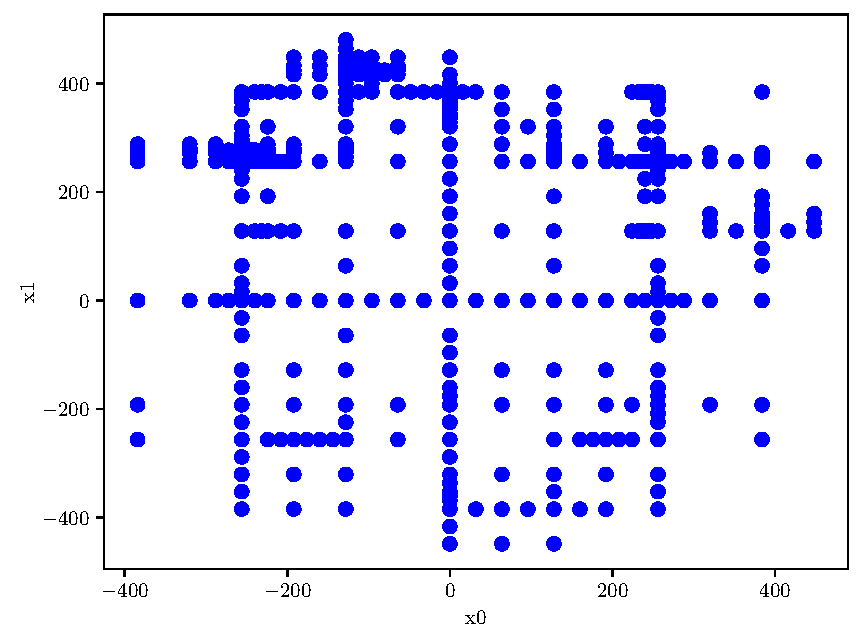
\includegraphics[width=\textwidth]{figures/Results/Sparse_grid_generation_results/Eggholder/tex_files/Eggholder_0_5}
		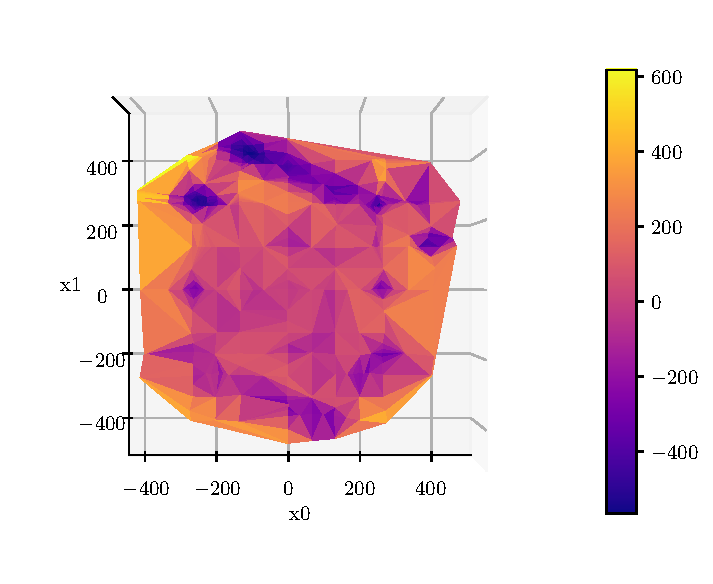
\includegraphics[width=\textwidth]{figures/Results/Sparse_grid_generation_results/Eggholder/tex_files/Eggholder_above_0_5}
		\caption{$ \gamma = 0.5 $}
		\label{fig:Egg_gamma_0_5}
	\end{subfigure}
	\begin{subfigure}{0.3\textwidth}
		\centering
		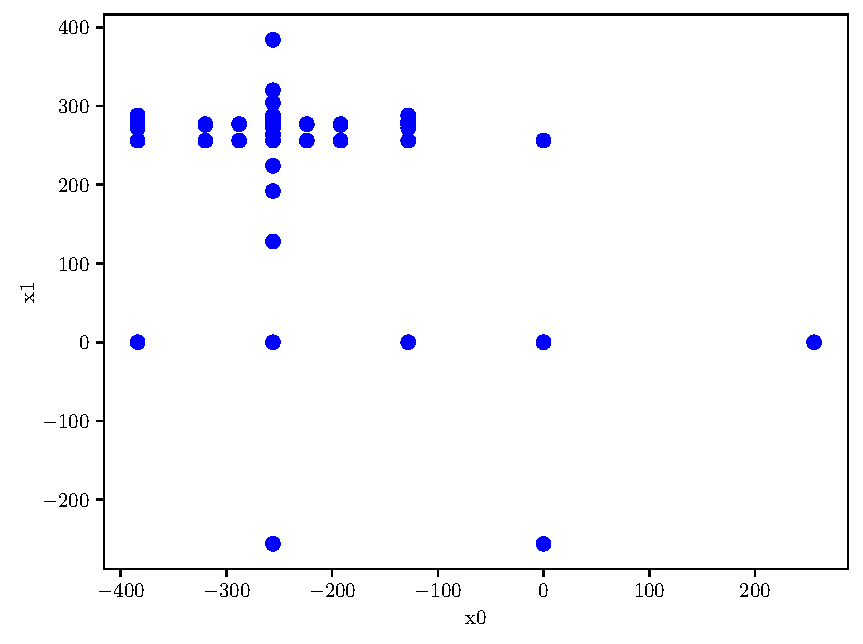
\includegraphics[width=\textwidth]{figures/Results/Sparse_grid_generation_results/Eggholder/tex_files/Eggholder_0}
		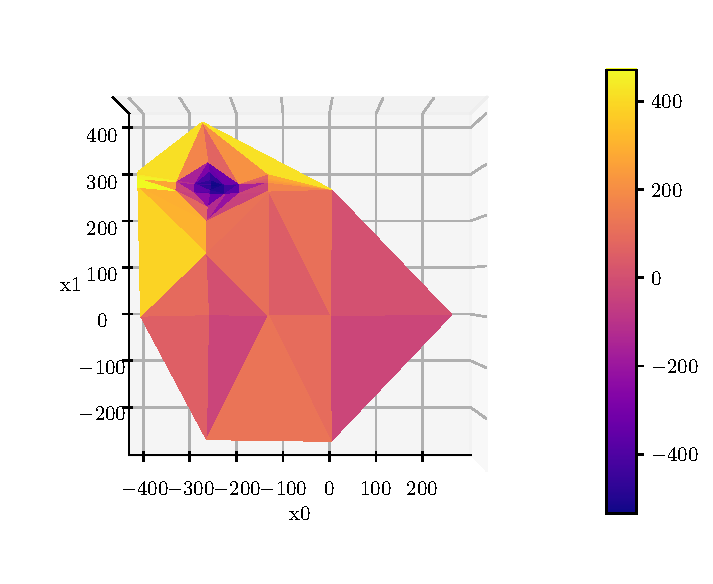
\includegraphics[width=\textwidth]{figures/Results/Sparse_grid_generation_results/Eggholder/tex_files/Eggholder_above_0}
		\caption{$ \gamma = 0.0 $}
		\label{fig:Egg_gamma_0}
	\end{subfigure}
	
	\caption{Sparse grid generation depending on the adaptivity parameter $ \gamma $ for the Eggholder function. In all cases, the same number of grid points is used. Here, in each of the 249 iterations, 4 new grid points are added resulting in a overall number of 997 function evaluations.}
	\label{fig:Eggholder_grid}
\end{figure}

In the first case with $ \gamma = 1.0 $, the grid is homogeneous and not adaptive at all. The grid points are distributed over the whole domain and the interpolated function looks very similar to the real plot from Figure \ref{fig:Eggholder}. 

The other extreme case is depicted in Figure \ref{fig:Egg_gamma_0}. There, the grid is maximally adaptive and really concentrated at the top left corner around $ (-260, 280) $. As it is known from Table \ref{tab:test_functions}, this is not where the optimal point is located. This behavior can be explained by the high exploitation throughout the iterations. With such a low adaptivity parameter, the grid points with low function values in the first iterations are mostly refined in the other iteration steps. 

The middle case with $ \gamma = 0.5 $ depicts a case where exploitation and exploration are more balanced. The grid points are more distributed than in the case of $ \gamma = 0.0 $ but there are also some regions where they are more refined, e.g. in the top left corner of the domain.

Note that in all three cases, the exact same number of grid points are evaluated. In this case, it is very hard for the sparse grid to find the real optimum because it is located at the border of the domain and it does not use grid points at the border. Also, the oscillatory nature of the function makes it hard to not concentrate on a local optimum which can happen in case of too high adaptivity. \newline

The next function used is the Rosenbrock function (see Figure \ref{fig:Rosenbrock}). Again, three different values for the adaptivity parameter are used. The results are depicted in Figure \ref{fig:Rosenbrock_grid}.

\begin{figure}[H]
	\begin{subfigure}{0.3\textwidth}
		\centering
		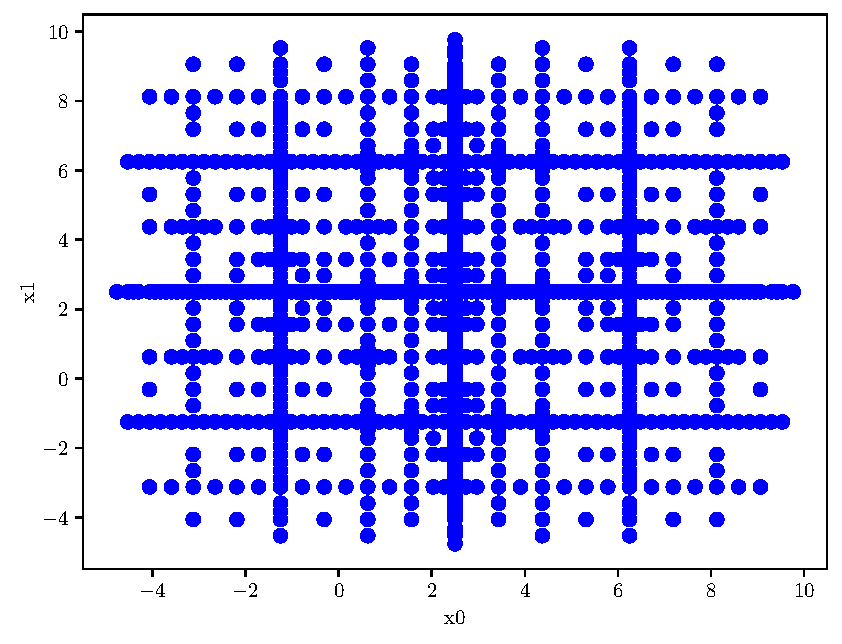
\includegraphics[width=\textwidth]{figures/Results/Sparse_grid_generation_results/Rosenbrock/tex_files/Rosenbrock_1}
		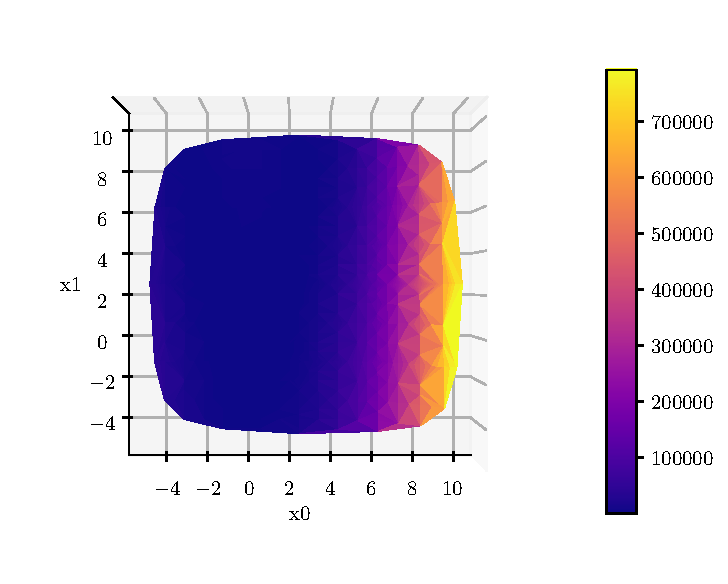
\includegraphics[width=\textwidth]{figures/Results/Sparse_grid_generation_results/Rosenbrock/tex_files/Rosenbrock_above_1}
		\caption{$ \gamma = 1.0 $}
		\label{fig:Ros_gamma_1}
	\end{subfigure}
	\begin{subfigure}{0.3\textwidth}
		\centering
		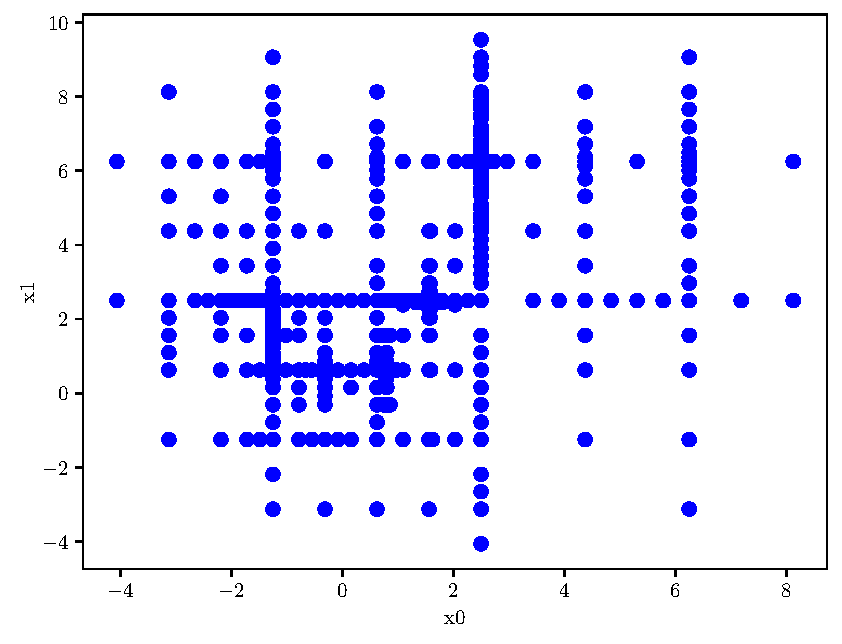
\includegraphics[width=\textwidth]{figures/Results/Sparse_grid_generation_results/Rosenbrock/tex_files/Rosenbrock_0_5}
		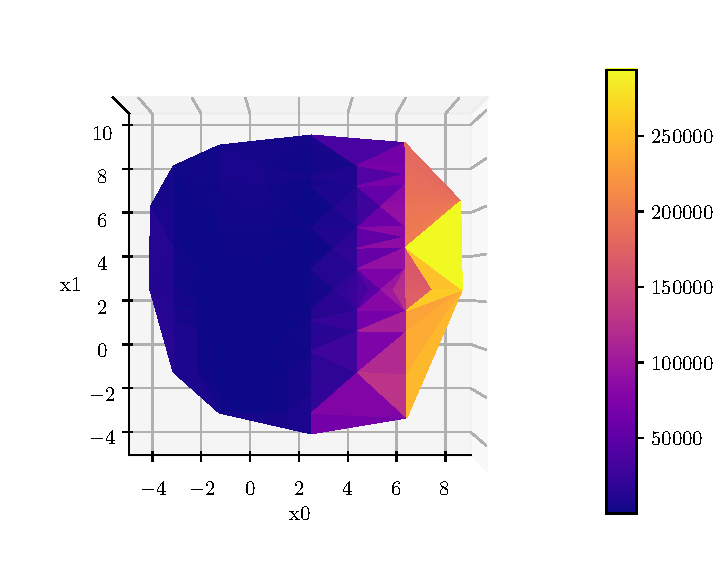
\includegraphics[width=\textwidth]{figures/Results/Sparse_grid_generation_results/Rosenbrock/tex_files/Rosenbrock_above_0_5}
		\caption{$ \gamma = 0.5 $}
		\label{fig:Ros_gamma_0_5}
	\end{subfigure}
	\begin{subfigure}{0.3\textwidth}
		\centering
		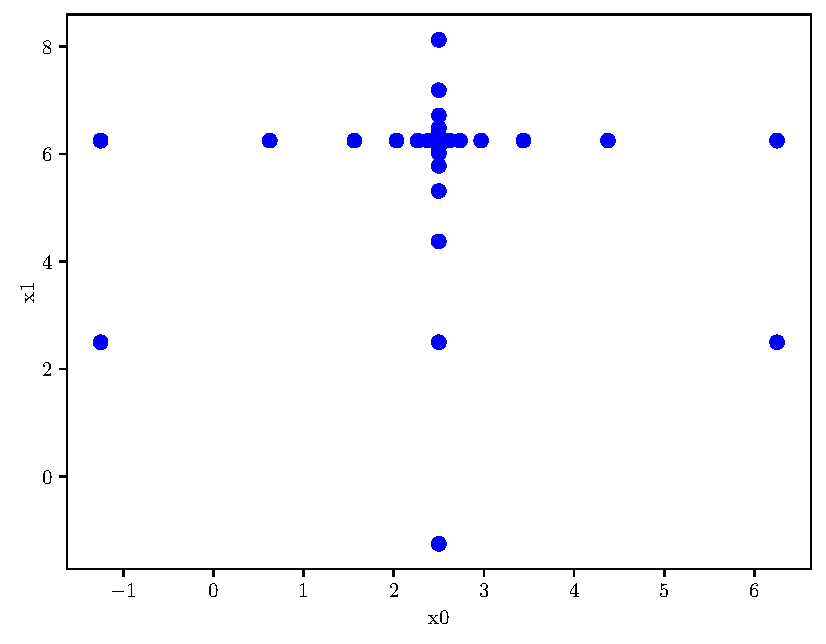
\includegraphics[width=\textwidth]{figures/Results/Sparse_grid_generation_results/Rosenbrock/tex_files/Rosenbrock_0}
		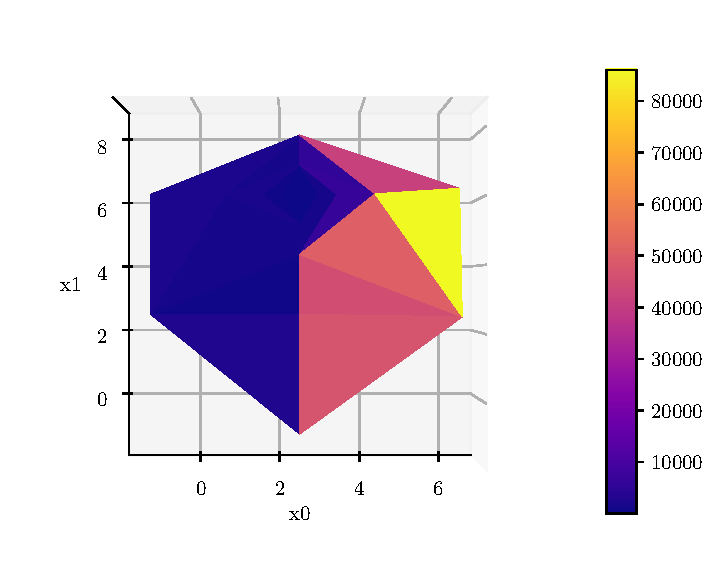
\includegraphics[width=\textwidth]{figures/Results/Sparse_grid_generation_results/Rosenbrock/tex_files/Rosenbrock_above_0}
		\caption{$ \gamma = 0.0 $}
		\label{fig:Ros_gamma_0}
	\end{subfigure}
	
	\caption{Sparse grid generation depending on the adaptivity parameter $ \gamma $ for the Rosenbrock function. In all cases, the same number of grid points is used. Here, in each of the 249 iterations, 4 new grid points are added resulting in a overall number of 997 function evaluations.}
	\label{fig:Rosenbrock_grid}
\end{figure}


The first fact that can be observed is that the sparse grid in the first case (Figure \ref{fig:Ros_gamma_1}) is exactly the same as the one for the Eggholder function (Figure \ref{fig:Egg_gamma_1}). This is due to the fact that this value of $ \gamma $ leads to a homogeneous sparse grid which is not dependent on the function used but rather the number of iterations for the grid generation. In this case, the interpolated function looks similar to the real function (Figure \ref{fig:Rosenbrock}). 

Now with decreasing value of $ \gamma $, the grid gets more and more inhomogeneous, while concentrating to refine smaller function values. The extreme case can be seen in Figure \ref{fig:Ros_gamma_0}, where the most grid points are next to the point $ (2.5, 6.25) $. After refining the first point in the middle, the one on top of it is getting refined all the time for the case $ \gamma = 0.0 $. Again, the sparse grid with $ \gamma = 0.5 $ is more balanced with more grid points on the left where the real optimum is located. \newline 


The last function used is the Rastrigin function (see Figure \ref{fig:Rastrigin} for the plot of the function and \ref{fig:Rastrigin_grid} for the resulting sparse grids). 

\begin{figure}[H]
	\begin{subfigure}{0.3\textwidth}
		\centering
		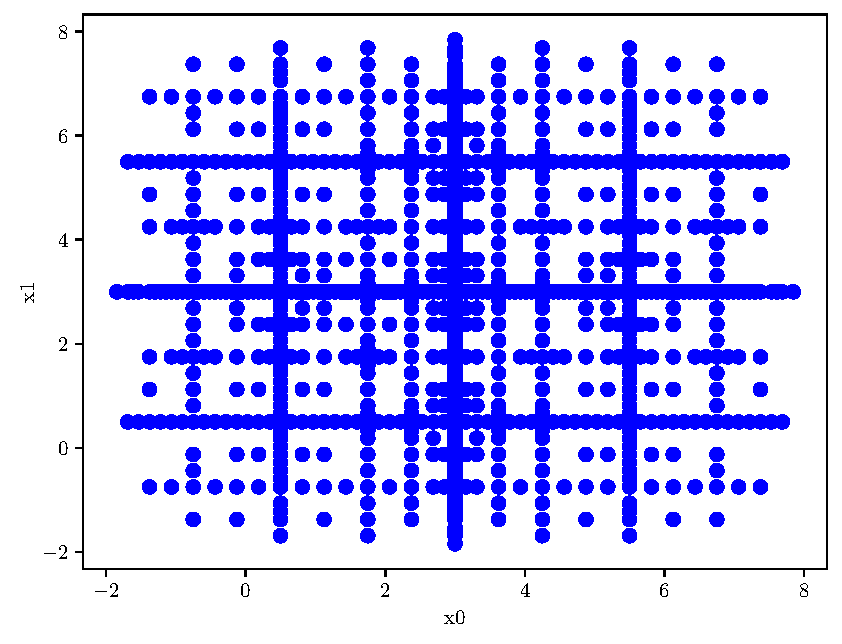
\includegraphics[width=\textwidth]{figures/Results/Sparse_grid_generation_results/Rastrigin/tex_files/Rastrigin_1}
		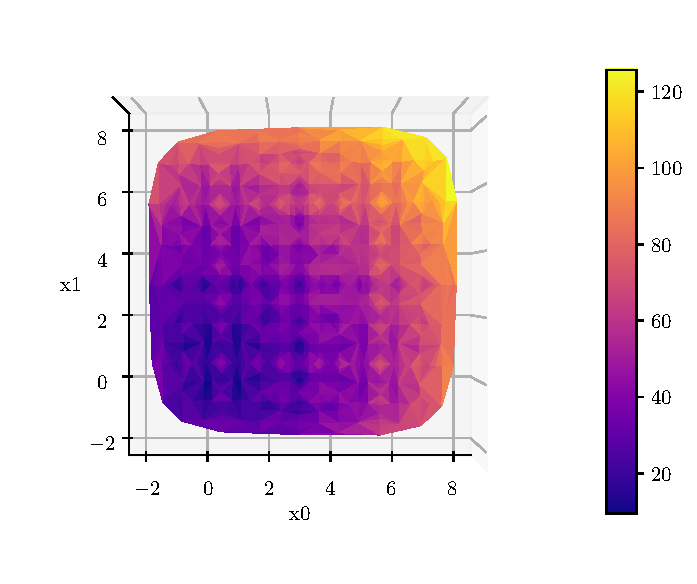
\includegraphics[width=\textwidth]{figures/Results/Sparse_grid_generation_results/Rastrigin/tex_files/Rastrigin_above_1}
		\caption{$ \gamma = 1.0 $}
		\label{fig:Ras_gamma_1}
	\end{subfigure}
	\begin{subfigure}{0.3\textwidth}
		\centering
		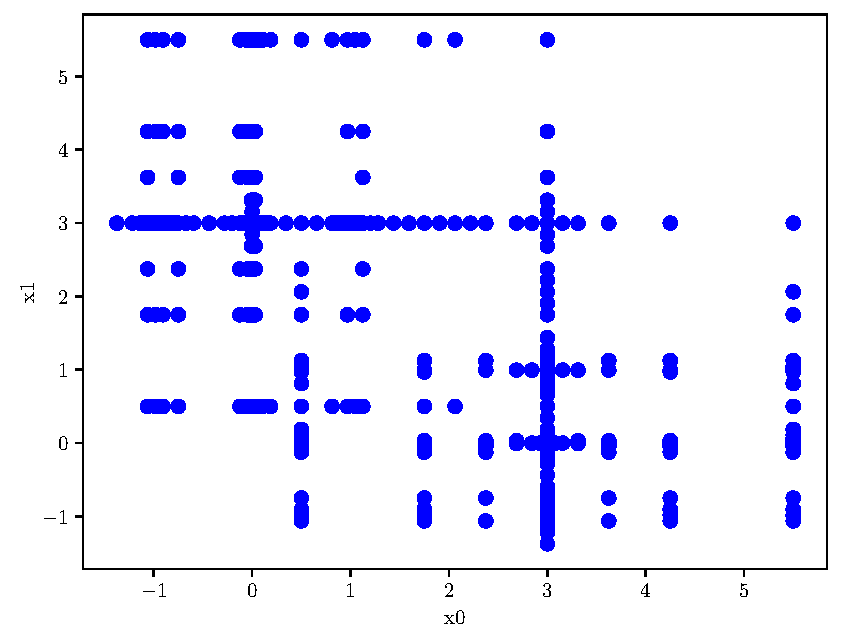
\includegraphics[width=\textwidth]{figures/Results/Sparse_grid_generation_results/Rastrigin/tex_files/Rastrigin_0_5}
		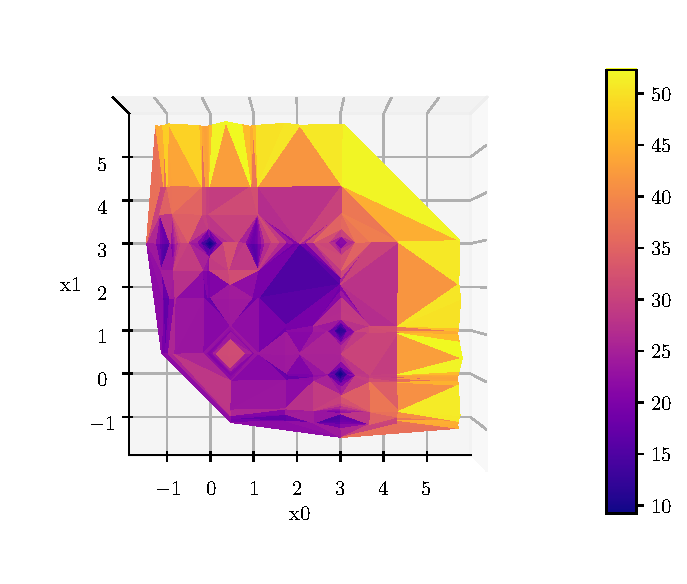
\includegraphics[width=\textwidth]{figures/Results/Sparse_grid_generation_results/Rastrigin/tex_files/Rastrigin_above_0_5}
		\caption{$ \gamma = 0.5 $}
		\label{fig:Ras_gamma_0_5}
	\end{subfigure}
	\begin{subfigure}{0.3\textwidth}
		\centering
		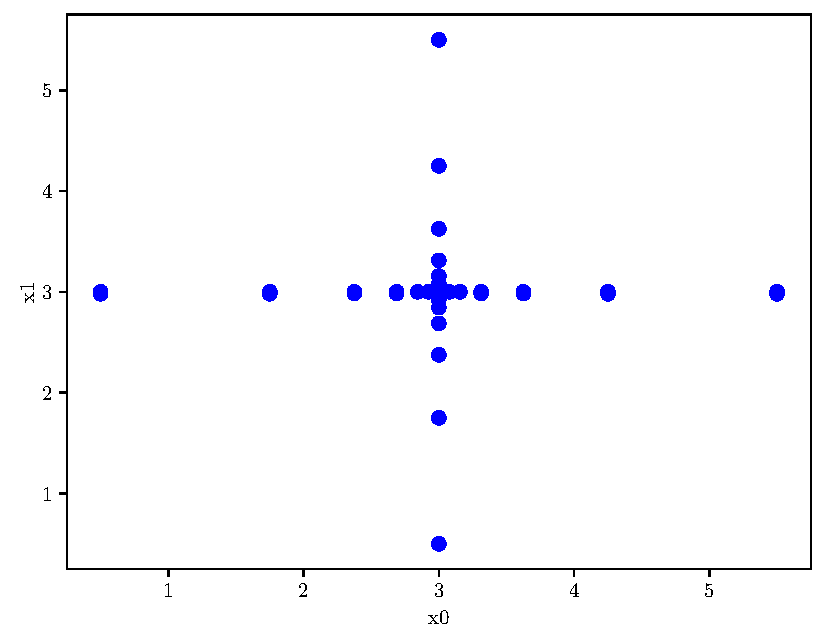
\includegraphics[width=\textwidth]{figures/Results/Sparse_grid_generation_results/Rastrigin/tex_files/Rastrigin_0}
		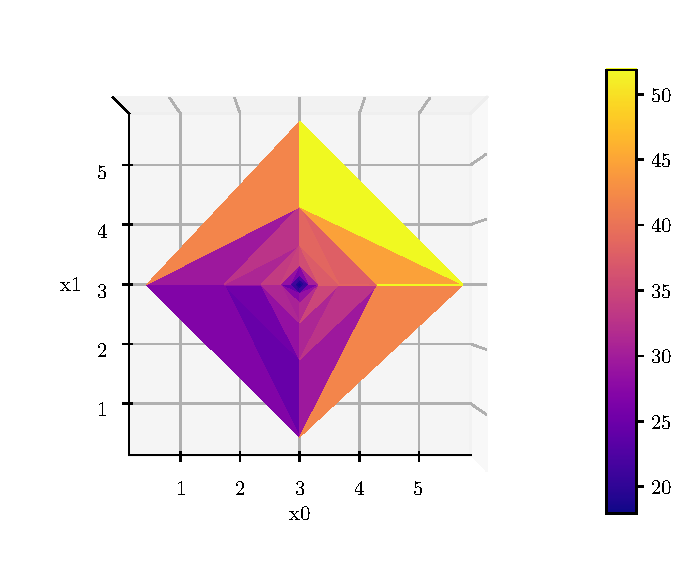
\includegraphics[width=\textwidth]{figures/Results/Sparse_grid_generation_results/Rastrigin/tex_files/Rastrigin_above_0}
		\caption{$ \gamma = 0.0 $}
		\label{fig:Ras_gamma_0}
	\end{subfigure}
	
	\caption{Sparse grid generation depending on the adaptivity parameter $ \gamma $ for the Rastrigin function. In all cases, the same number of grid points is used. Here, in each of the 249 iterations, 4 new grid points are added resulting in a overall number of 997 function evaluations.}
	\label{fig:Rastrigin_grid}
\end{figure}

As in the previous two cases, the sparse grid is exactly the same for $ \gamma = 1.0 $. We can also see the same behavior for a decreasing adaptivity parameter. For $ \gamma = 0.0 $, only the grid point in the center is refined in all steps. In the middle case, the grid looks more balanced with a tendency to the bottom left corner.  \newline 


In conclusion, these experiments show that the value for the adaptivity parameter strongly influences the grid generation and the resulting optimal value found by the algorithm. In general, this trade-off between exploitation with trying to find a solution fast and exploration with reconstructing the function in the whole domain can be balanced with this adaptivity parameter. \newline

In the following, the goal is to further analyze this adaptivity parameter. For each of the three test functions, experiments with $ \gamma \in \{0.0, 0.25, 0.5, 0.75, 1.0\} $ are made. The error of the optimum found by the grid is calculated depending on the number of grid points used. It is evaluated with 
\begin{equation}
 Error = f(x_{opt}^*) - f(x_{opt}) 
\end{equation}
where $ x_{opt}^* $ is the optimal point found by the sparse grid and $ x_{opt} $ is the real optimum. Figure \ref{fig:test_functions_plot} shows the resulting Errors depending on the number of grid points used. The top left plot is for the Eggholder function, the one on the top right belongs to the Rosenbrock function and the bottom one corresponds to the Rastrigin function. \newline

\begin{figure}[H]
	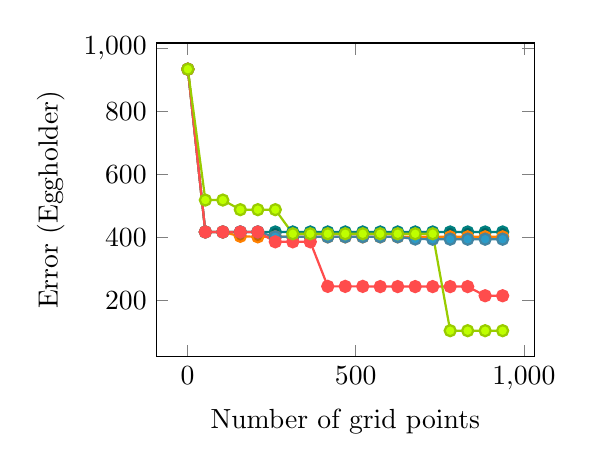
\begin{tikzpicture}
		\begin{axis}[
			xlabel = Number of grid points,
			ylabel = Error (Eggholder),
			scale=0.7,
			cycle list name=exotic,
			]
			
			\addplot+[mark=*, style=thick] coordinates {(1,934.1803628147137)(53,416.6753127436343)(105,416.67517650515606)(157,416.67517650515606)(209,416.6751765051557)(261,416.6751765051555)(313,416.67517650515515)(365,416.67517650515583)(417,416.67517650515606)(469,416.67517650515515)(521,416.67517650515595)(573,416.6751765051555)(625,416.6751765051557)(677,416.6751765051554)(729,416.6751765051555)(781,416.67517650515595)(833,416.6751765051555)(885,416.6751765051557)(937,416.6751765051557)};
			
			\addplot+[mark=*, style=thick]  coordinates 
			{(1,934.1803628147137)(53,416.6753127436343)(105,416.67517650515606)(157,402.86392358909313)(209,401.165066632121)(261,401.16506654901593)(313,401.16506654901764)(365,401.1650665490138)(417,401.1650665490125)(469,401.1650665490105)(521,401.16506654901195)(573,401.1650665490175)(625,401.16506654902184)(677,401.16506654901843)(729,401.16506654901593)(781,401.1650665490224)(833,401.16506654902105)(885,401.1650665490139)(937,401.1650665490138)};
			
			\addplot+[mark=*, style=thick]   coordinates 
			{(1,934.1803628147137)(53,416.6753127436343)(105,416.67517650515595)(157,416.67517650515595)(209,416.6751765051556)(261,401.16506923718293)(313,401.1650665490133)(365,401.1650665490122)(417,401.16506654901445)(469,401.1650665490125)(521,401.16506654901264)(573,401.16506654901264)(625,401.1650665490216)(677,394.1301115312152)(729,393.6496427441624)(781,393.6444455890784)(833,393.6437130885647)(885,393.6437130885688)(937,393.6437130885528)};
			
			\addplot+[mark=*, style=thick]  coordinates
				{(1,934.1803628147137)(53,416.680649645461)(105,416.67519174547897)(157,416.6751765051557)(209,416.6751765051554)(261,385.37674780492864)(313,385.35652906792404)(365,385.3565290679238)(417,243.68003942485666)(469,243.67992321536838)(521,243.67992321536633)(573,243.01108728703605)(625,242.99463717547087)(677,242.99463717547076)(729,242.99463717547087)(781,242.99463717546962)(833,242.99463717546973)(885,213.83490792055488)(937,213.834907133721)};
			
			\addplot+[mark=*, style=thick]  coordinates 
			{(1,934.1803628147137)(53,518.1399491004825)(105,518.1399491004823)(157,487.54622876272015)(209,487.54622876272003)(261,487.54622876272)(313,410.9897867087419)(365,410.9897867087424)(417,410.9897867087427)(469,410.9897867087419)(521,410.9897867087424)(573,410.98978670874214)(625,410.9897867087425)(677,410.9897867087424)(729,410.9897867087428)(781,102.75674102278083)(833,102.7567410227864)(885,102.75674102278651)(937,102.75674102279345)};
			
		\end{axis}
	\end{tikzpicture}
	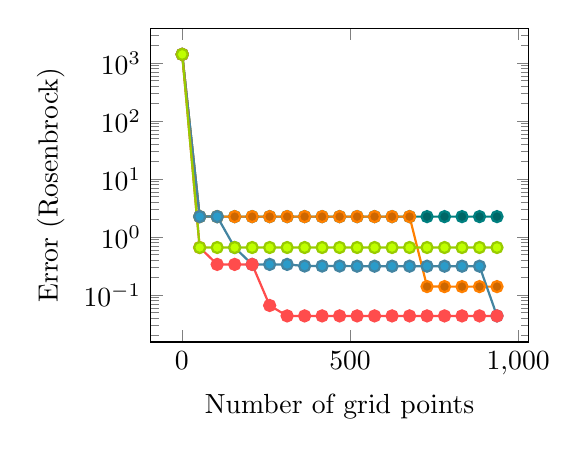
\begin{tikzpicture}
		\begin{axis}[
			xlabel = Number of grid points,
			ylabel = Error (Rosenbrock),
			scale = 0.7,
			ymode=log,
			cycle list name=exotic,
			]
			
			\addplot+[mark=*, style=thick] coordinates {(1,1408.5)(53,2.25)(105,2.2491001457701714)(157,2.2491001457701714)(209,2.2491001457722626)(261,2.2491001457672675)(313,2.249100145771435)(365,2.249100145769731)(417,2.2491001457715205)(469,2.249100145772637)(521,2.2491001457718287)(573,2.249100145770883)(625,2.2491001457697997)(677,2.24910014577051)(729,2.2491001457706186)(781,2.249100145769841)(833,2.2491001457692894)(885,2.249100145769003)(937,2.2491001457706337)};
			
			\addplot+[mark=*, style=thick]  coordinates 
			{(1,1408.5)(53,2.25)(105,2.2491001457701714)(157,2.2491001457701714)(209,2.2491001457721036)(261,2.2491001457695767)(313,2.249100145770952)(365,2.2491001457690514)(417,2.2491001457697983)(469,2.2491001457687094)(521,2.2491001457707274)(573,2.249100145770689)(625,2.2491001457705138)(677,2.249100145770712)(729,0.13999960097248135)(781,0.13973409018662308)(833,0.1397340901880652)(885,0.1397340901910032)(937,0.13973409019308297)};
			
			\addplot+[mark=*, style=thick]   coordinates 
			{(1,1408.5)(53,2.25)(105,2.2491001457701714)(157,0.65972900390625)(209,0.33738539328720274)(261,0.337384855010467)(313,0.3373848550084554)(365,0.3164062500005624)(417,0.3160824744022442)(469,0.316082474402264)(521,0.3143689789723247)(573,0.31436571579881106)(625,0.3143657157996295)(677,0.3143657157842261)(729,0.3143657158217291)(781,0.31436571578093114)(833,0.3143657158159762)(885,0.31436571582376066)(937,0.04369918730841191)};
			
			\addplot+[mark=*, style=thick]  coordinates
			{(1,1408.5)(53,0.65972900390625)(105,0.33738539328578554)(157,0.3373848550099865)(209,0.33738485500900234)(261,0.06609634402749087)(313,0.04368661484965771)(365,0.043686614913836186)(417,0.043686614861208506)(469,0.04368661485251346)(521,0.04368661485326686)(573,0.04368661485538938)(625,0.04368661485308678)(677,0.043686614838481574)(729,0.04368661486120118)(781,0.04368661488831904)(833,0.043686614839174354)(885,0.04368661486845582)(937,0.04368661486256009)};
			
			\addplot+[mark=*, style=thick]  coordinates 
			{(1,1408.5)(53,0.65972900390625)(105,0.65972900390625)(157,0.65972900390625)(209,0.6597290039064774)(261,0.6597290039068184)(313,0.65972900390625)(365,0.65972900390625)(417,0.65972900390625)(469,0.6597290039065911)(521,0.6597290039067047)(573,0.6597290039064774)(625,0.6597290039064774)(677,0.6597290039067047)(729,0.6597290039067047)(781,0.6597290039064774)(833,0.65972900390625)(885,0.6597290039065911)(937,0.6597290039065911)};
			
		\end{axis}
	\end{tikzpicture}
	\centering
	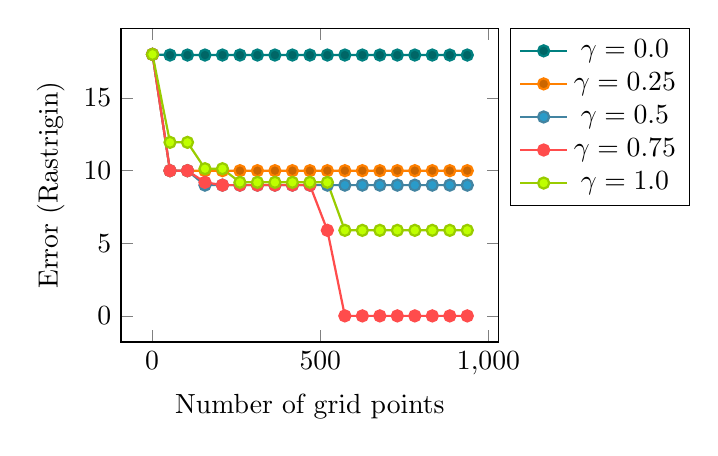
\begin{tikzpicture}
		\begin{axis}[
			xlabel = Number of grid points,
			ylabel = Error (Rastrigin),
			scale = 0.7,
			cycle list name=exotic,
			legend pos=outer north east,
			]
			
			\addplot+[mark=*, style=thick] coordinates{(1,18.0)(53,17.954603830243304)(105,17.954601241487484)(157,17.954601241487484)(209,17.95460124148829)(261,17.954601241487573)(313,17.95460124148752)(365,17.954601241487435)(417,17.95460124148751)(469,17.954601241487524)(521,17.954601241487467)(573,17.954601241487463)(625,17.954601241487506)(677,17.954601241487463)(729,17.95460124148793)(781,17.954601241488138)(833,17.954601241487886)(885,17.954601241487513)(937,17.954601241488046)};
			
			\addplot+[mark=*, style=thick]  coordinates 
			{(1,18.0)(53,9.995024358227056)(105,9.994959057644616)(157,9.994959057644616)(209,9.994959057646103)(261,9.99495905764463)(313,9.994959057644524)(365,9.99495905764453)(417,9.99495905764462)(469,9.994959057644579)(521,9.994959057644468)(573,9.994959057644502)(625,9.994959057644628)(677,9.994959057644607)(729,9.99495905764461)(781,9.994959057644595)(833,9.99495905764462)(885,9.994959057644616)(937,9.994959057644667)};
			
			\addplot+[mark=*, style=thick]   coordinates 
			{(1,18.0)(53,9.995024358227056)(105,9.994959057644618)(157,9.000000184767032)(209,9.000000000721773)(261,9.0000000007217)(313,9.000000000721338)(365,9.000000000721721)(417,9.00000000072155)(469,9.00000000072114)(521,9.000000000721972)(573,9.000000000721784)(625,9.00000000072177)(677,9.000000000721762)(729,9.00000000072182)(781,9.000000000721915)(833,9.000000000721828)(885,9.000000000721684)(937,9.000000000721721)};
			
			\addplot+[mark=*, style=thick]  coordinates
			{(1,18.0)(53,9.995597577515051)(105,9.994959320973711)(157,9.193123758467696)(209,9.000000000721291)(261,9.000000000720725)(313,9.00000000073414)(365,9.000000000715445)(417,9.000000000715788)(469,9.00000000072136)(521,5.889114376269022)(573,0.001513592628570368)(625,1.9994962252604298e-07)(677,1.2455895805700494e-08)(729,1.2778394708011167e-08)(781,1.2291804361994243e-08)(833,1.179890717001382e-08)(885,1.251678228282502e-08)(937,1.231146666513552e-08)};
			
			\addplot+[mark=*, style=thick]  coordinates 
			{(1,18.0)(53,11.944557188134524)(105,11.944557188134521)(157,10.130623758467696)(209,10.130623758467692)(261,9.193123758467797)(313,9.193123758467703)(365,9.193123758467696)(417,9.1931237584677)(469,9.1931237584677)(521,9.193123758467692)(573,5.8891143762690925)(625,5.889114376269034)(677,5.88911437626902)(729,5.889114376269047)(781,5.889114376269048)(833,5.889114376269062)(885,5.889114376269007)(937,5.889114376269115)};
			
			\legend{$ \gamma = 0.0 $, $ \gamma = 0.25 $, $ \gamma = 0.5 $, $ \gamma = 0.75 $, $ \gamma = 1.0 $,}
			
		\end{axis}
	\end{tikzpicture}
	\caption{ Influence of the adaptivity parameter on the error (difference to the actual optimal value) of the optimum found by the sparse grid. }	
	\label{fig:Functions_results}
\end{figure}

For all three test functions, a value $ 0.75 \le \gamma \le 1.0 $ leads to the smallest error with higher number of grid points. This means that a fast exploitation is not good for finding the global optimum. For the Rastrigin function, the most adaptive sparse grid does not even lead to a smaller error with up to 1000 grid points. This is the same example as in Figure \ref{fig:Ras_gamma_0}, where only the center point is refined. Note that by now, no optimization algorithm is applied on top of the sparse grid. For further experiments, the adaptivity parameter will be set to $ \gamma = 0.85 $. \newline 

\subsection{Local and Global Optimization}

The next improvement is to add optimizers after the grid generation phase. There are two different types of algorithms. The first one is local optimization, for example, based on the gradient like the gradient descent. The second one is global optimization. An example therefore is to use a multi-start approach by trying out multiple different starting points for the algorithm. These various initial values can be uniformly distributed in the domain. The following experiments show how the error (difference between optimum found by the algorithm and actual optimal function value) behaves with a higher number of grid points of the underlying sparse grid. As a local optimization algorithm, gradient descent is used. The starting point for this algorithm is set to the point of the sparse grid where the smallest function value was found. For the global optimization, a multi-start approach with 20 equally distributed starting points is used. The concrete algorithm is the nelder mead optimization as described in \ref{Optimization_algorithms}. The number of function evaluations used in this method, as well as the number of steps for gradient descent is set to 1000. One important parameter for the optimization is the degree of the B-splines used on the sparse grid. The resulting errors depending on the number of grid points for the degrees 2, 3, and 5 can be seen in Figure \ref{fig:Optimizer_results}. The Rosenbrock function is used in all cases.

\begin{figure}[H]
	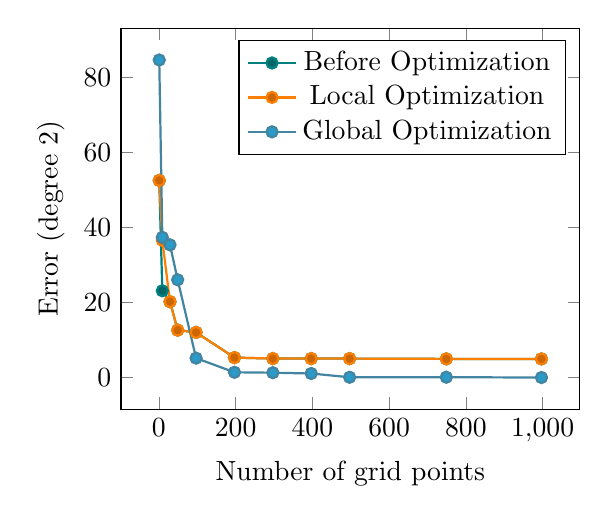
\begin{tikzpicture}
		\begin{axis}[
			xlabel = Number of grid points,
			ylabel = Error (degree 2),
			scale=0.85,
			cycle list name=exotic,
			legend pos=north east,
			]
			
			\addplot+[mark=*, style=thick] coordinates
			{(1,52.5) (9,23.124999999999993) (29,20.221948342338713) (49,12.642146873903034) (97,12.037968800252116) (197,5.324940782205941) (297,5.070573664357864) (397,5.059483529507994) (497,5.059483529509992) (749,4.981978981445401) (997,4.975134049661977) };
			
			\addplot+[mark=*, style=thick]  coordinates 
			{(1,52.5) (9,36.56247783900481) (29,20.221948342338713) (49,12.642146873903027) (97,12.037968800252123) (197,5.324940782205946) (297,5.070573664357985) (397,5.059483529510453) (497,5.059483529510453) (749,4.981978981455729) (997,4.975134049663653) };
			
			\addplot+[mark=*, style=thick]   coordinates 
			{(1,84.58773867867924) (9,37.34881542254573) (29,35.353118558881526) (49,26.048828056455157) (97,5.180279637187814) (197,1.4141172901666579) (297,1.3031251937216908) (397,1.0903873189756652) (497,0.08680369103412033) (749,0.10422400147368194) (997,0.020853342869873615) };
			
			\legend{Before Optimization, Local Optimization, Global Optimization}
			
		\end{axis}
	\end{tikzpicture}
	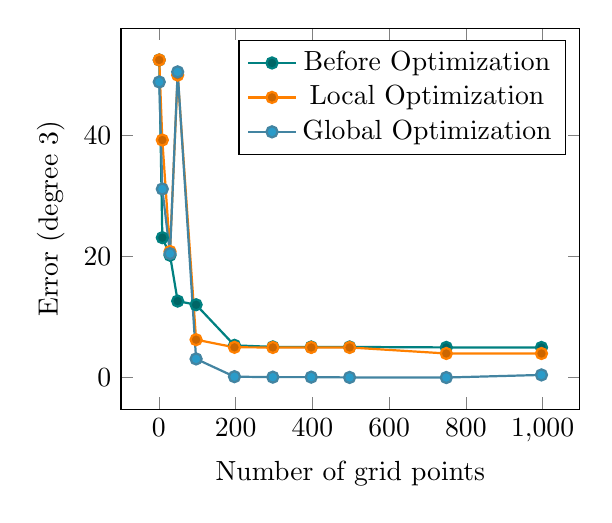
\begin{tikzpicture}
		\begin{axis}[
			xlabel = Number of grid points,
			ylabel = Error (degree 3),
			scale=0.85,
			cycle list name=exotic,
			legend pos=north east,
			]
			
			\addplot+[mark=*, style=thick] coordinates
			{(1,52.5) (9,23.124999999999986) (29,20.221948342338727) (49,12.642146873903025) (97,12.037968800252077) (197,5.324940782206068) (297,5.070573664356438) (397,5.059483529515382) (497,5.059483529505752) (749,4.9819789814573205) (997,4.975134049660271) };
			
			\addplot+[mark=*, style=thick]  coordinates 
			{(1,52.5) (9,39.26658373479667) (29,20.847171449176678) (49,49.99973745586844) (97,6.259687480962173) (197,5.002154846904871) (297,4.975751718068931) (397,4.975746034104377) (497,4.975697508130967) (749,3.980892241733912) (997,3.979835850885795) };
			
			\addplot+[mark=*, style=thick]   coordinates 
			{(1,48.864612088186476) (9,31.16918203994022) (29,20.48853217431511) (49,50.53387608332728) (97,3.0805866327728566) (197,0.14445847530268452) (297,0.06980177032781754) (397,0.06988725538127483) (497,0.02077395004058502) (749,0.003850124352695161) (997,0.4352002384999345) };
			
			\legend{Before Optimization, Local Optimization, Global Optimization}
			
		\end{axis}
	\end{tikzpicture}
	\centering
	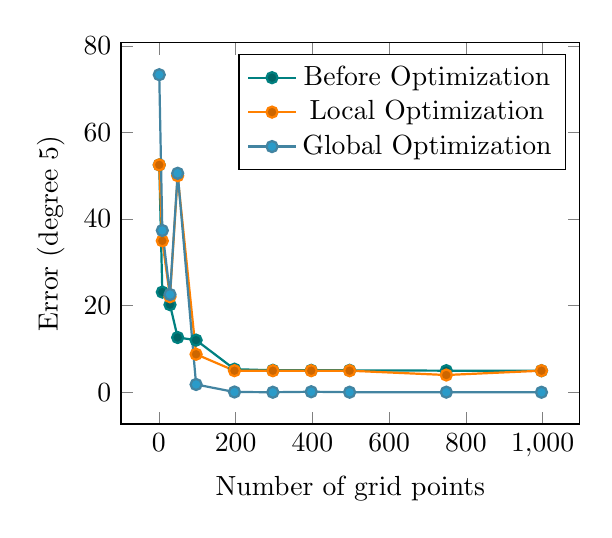
\begin{tikzpicture}
		\begin{axis}[
			xlabel = Number of grid points,
			ylabel = Error (degree 5),
			scale=0.85,
			cycle list name=exotic,
			legend pos=north east,
			]
			
			\addplot+[mark=*, style=thick] coordinates
			{(1,52.5) (9,23.124999999999996) (29,20.221948342338706) (49,12.642146873903044) (97,12.037968800252427) (197,5.324940782206359) (297,5.070573664363549) (397,5.059483529512068) (497,5.059483529510554) (749,4.981978981456664) (997,4.975134049668072) };
			
			\addplot+[mark=*, style=thick]  coordinates 
			{(1,52.5) (9,34.964270829168846) (29,22.048613242940117) (49,49.999815285630675) (97,8.771776029715767) (197,4.977579661397227) (297,4.9749420077761) (397,4.974930572100956) (497,4.974940210636003) (749,3.9798360656238323) (997,4.974790247773939) };
			
			\addplot+[mark=*, style=thick]   coordinates 
			{(1,73.32956404214876) (9,37.355007206361236) (29,22.57998988395788) (49,50.570154840256905) (97,1.7957114981045024) (197,0.059327067234512754) (297,0.0044097596433303465) (397,0.11308692978262513) (497,0.008066444905090009) (749,0.02197720207793452) (997,0.002142203898742423) };
			
			\legend{Before Optimization, Local Optimization, Global Optimization}
			
		\end{axis}
	\end{tikzpicture}
	\caption{ Optimization error for different algorithms depending on the number of grid points in two dimensions. The plots show the results with degree 2 (top left), degree 3 (top right) and degree 5 (bottom). The Rastrigin function was used. }	
	\label{fig:Optimizer_results}
\end{figure}

In all three cases, the errors of the local and global optimizers first increase with increasing number of grid points until about 100 to 200 function evaluations are done. After that, both local and global optimization algorithms are at least as good as the result found by the sparse grid. With increasing number of grid points, the global optimization finds the best solution in all cases with degrees 2, 3, and 5. \newline 

The visualization in Figure \ref{fig:optimizers_visualized} indicates why the global optimizer achieves the best results for a high number of sparse grid points. 
\begin{figure}[H]
	\centering
	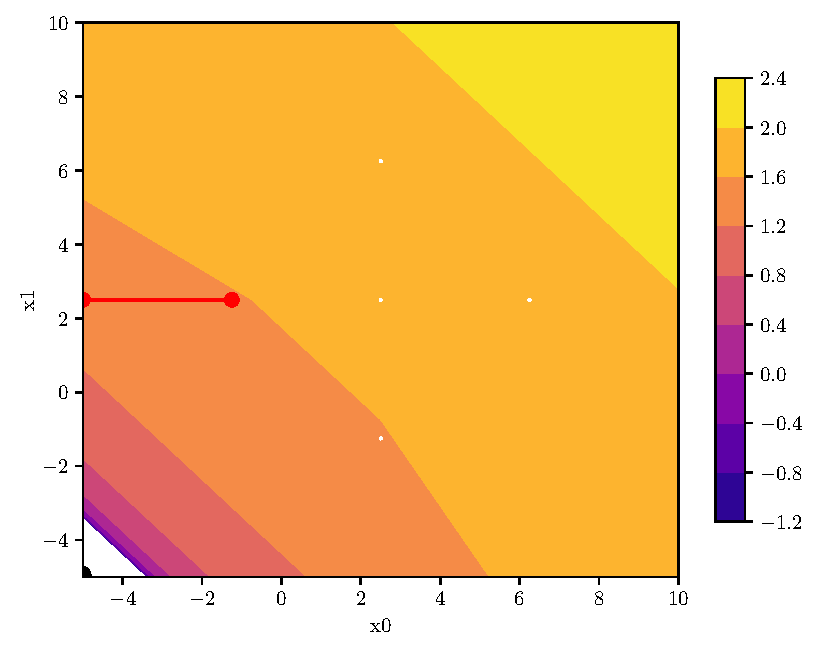
\includegraphics[width=0.31\textwidth]{figures/Results/Testfunctions/Optimizer_visualization/Optimizers_visualization5}
	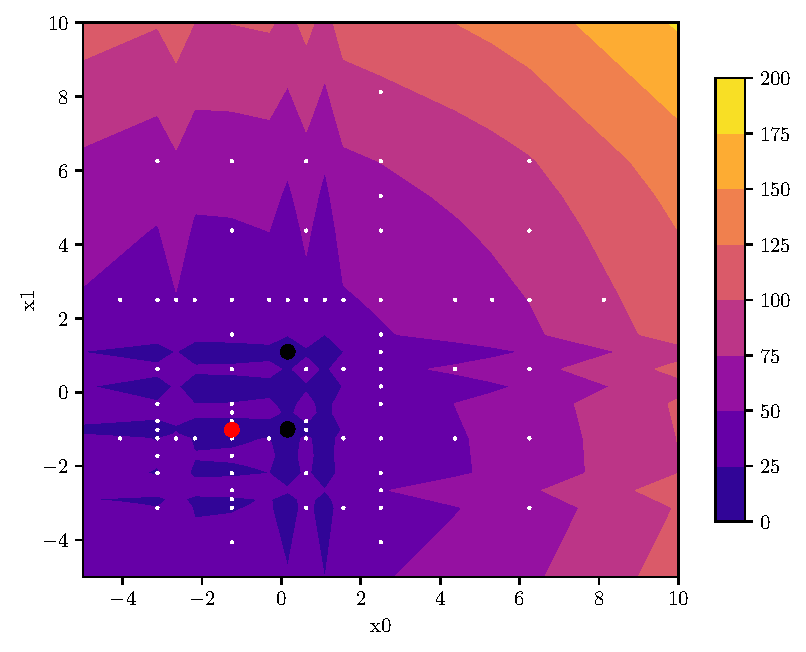
\includegraphics[width=0.31\textwidth]{figures/Results/Testfunctions/Optimizer_visualization/Optimizers_visualization80}
	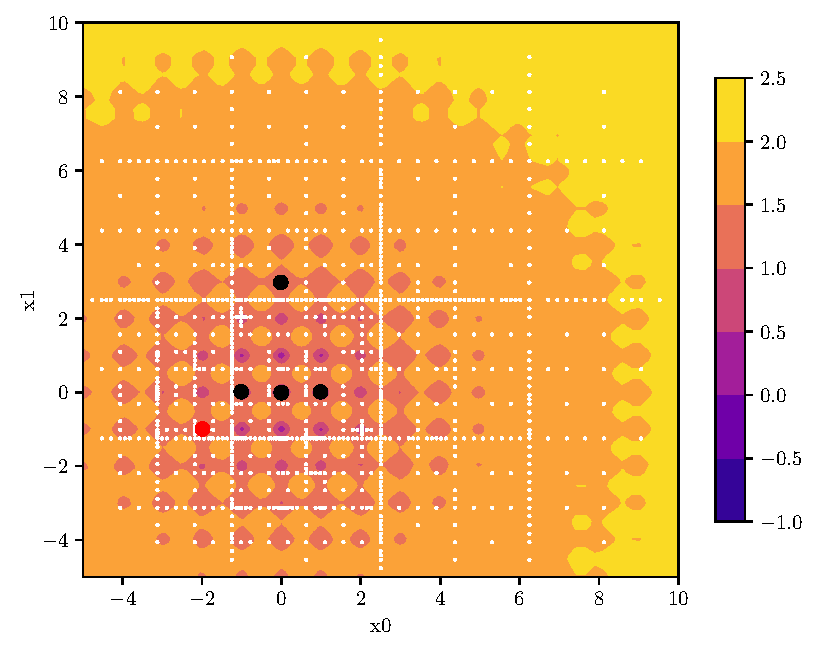
\includegraphics[width=0.31\textwidth]{figures/Results/Testfunctions/Optimizer_visualization/Optimizers_visualization1000}
	
	\caption{Resulting optimal points from local (red points) and global (black points) optimization algorithm. In the background, the contour of the interpolated function is depicted with the corresponding sparse grid points in white. The left one has 5 grid points, the one in the center 77, and the right one 997. The degree of the B-splines on the sparse grid is 2. }
	\label{fig:optimizers_visualized}
\end{figure}

In the left example of Figure \ref{fig:optimizers_visualized} with 5 sparse grid points, the result of the local optimizer is at the left border of the domain as indicated by the red line which connects the different steps of the algorithm. All resulting optimal points found by the multi-start approach are located in the lower left corner. Note that the interpolated function is not very similar to the original one (see Figure \ref{fig:Rastrigin}) because of the low number of grid points. 

With an increasing number of these basis points, both algorithms find a better solution to the problem. In the center plot of Figure \ref{fig:optimizers_visualized}, 77 grid points were used and the interpolated contour looks more oscillatory and more similar to the original function. The local and global algorithms find different optimal points in this case. 

In the right example of Figure \ref{fig:optimizers_visualized}, 997 grid points were used and the contour already looks very similar to the function plot. There are many candidates of the global optimizer and so	me of them are near to the actual optimal point which is located at $ (0, 0) $. 


The exact solutions of each algorithm can be seen in Table \ref{tab:optimizer_vis_function}.
\begin{table}[h!]
	\caption{ Overview over the exact solutions found by the local and global optimizer for the same problem as in Figure \ref{fig:optimizers_visualized}. The actual optimum is at (0, 0), with function value 0 (see Table \ref{tab:test_functions}).}
	\label{tab:optimizer_vis_function}
	\centering
	\begin{tabular}{|c c c c c|} 
		\hline
		Number grid points & Optimizer & Coordinates & Interpolated value & Actual value \\
		\hline
		5 & Local &  (-5,2.5)  &  23.125  &  51.25  \\
		5 & Global &  (-4.998,-4.971)  &  -6.191  &  49.862  \\
		77 & Local &  (-1.25,-1.016)  &  12.642  &  12.642  \\
		77 & Global &  (0.157,-1.006)  &  5.756  &  5.514  \\
		997 & Local &  (-1.990,-0.994)  &  4.975  &  4.975  \\
		997 & Global & \textbf{(-0.014,-0.002)} & 0.151 & \textbf{0.042} \\
		\hline
	\end{tabular}
\end{table}

The big advantage of the global optimizer is that multiple starting points are used so that the chance of reaching the global minimum is very high. Especially for a high number of grid points used, this is the case. While the local optimizer only finds a local minimum (see Figure \ref{fig:optimizers_visualized}, red dot at (-1.99, -0.994)), the global optimizer finds multiple candidates at more than one local minimum. One of them is very near to the global optimal point in this case (see Figure \ref{fig:optimizers_visualized}, black dot at (0.002, 0.013)). \newline 


One approach is to combine all three resulting points with their corresponding function value. The overall optimal point is then just set to the one with the smallest function value. \newline 

The inputs of the previous experiments were all just two-dimensional. The following ones analyze the impact of the dimension on the performance of the algorithm. Therefore, the Rastrigin function is optimized, again with increasing number of grid points. The degree of the B-splines used on the sparse grid is set to 5 and for the adaptivity parameter, we set $ \gamma = 0.85 $. The results are depicted in Figure \ref{fig:Dimensions_results}.


\begin{figure}[H]
	\centering
	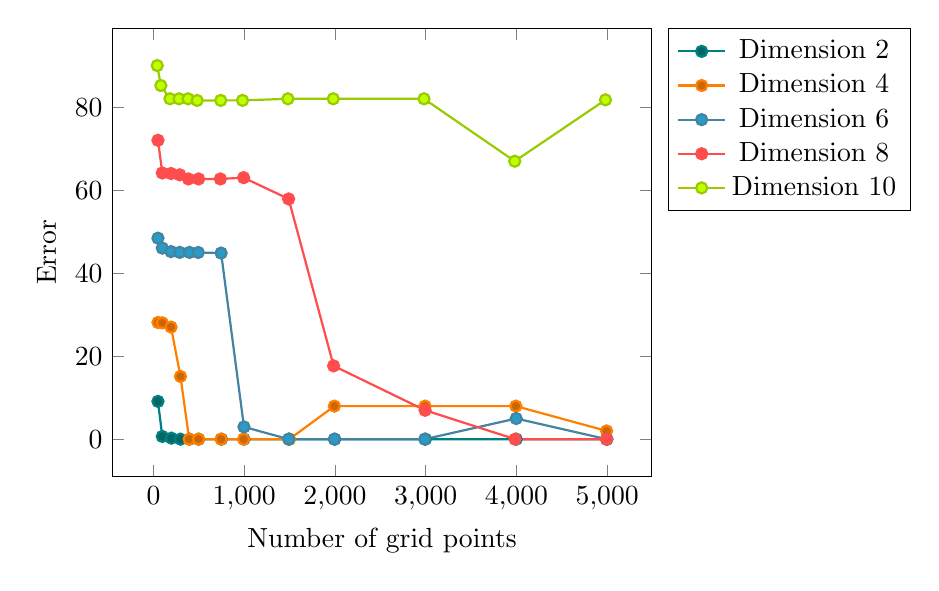
\begin{tikzpicture}
		\begin{axis}[
			xlabel = Number of grid points,
			ylabel = Error,
			scale=1,
			cycle list name=exotic,
			legend pos=outer north east,
			]
			
			\addplot+[mark=*, style=thick] coordinates
			{(49,9.101448500006125) (97,0.6579925771421742) (197,0.24877350577453328) (297,0.004037953576528253) (397,0.00025859422627760864) (497,1.7408297026122455e-13) (749,7.460698725481052e-14) (997,3.481659405224491e-13) (1497,5.044853423896711e-13) (1997,2.1316282072803006e-14) (2997,3.652389892749852e-06) (3997,2.8704901623655132e-05) (4997,5.787840197764794e-07) };
			
			\addplot+[mark=*, style=thick]  coordinates 
			{(49,28.11190602660223) (97,28.027731473104676) (193,27.012106473104676) (297,15.113252690760966) (393,9.600766347261924e-06) (497,1.6991705820146308e-09) (745,2.1316282072803006e-14) (993,8.952838470577262e-13) (1497,5.101696842757519e-12) (1993,7.959662418317201) (2993,7.959662532446124) (3993,7.959662444938445) (4993,1.989918226969806) };
			
			\addplot+[mark=*, style=thick]   coordinates 
			{(49,48.423119589928916) (97,46.02773147310465) (193,45.19017740517299) (289,45.000002956271466) (397,45.00000295627026) (493,44.97832419159962) (745,44.83586659446601) (997,2.9518635934690423) (1489,1.2755663192365319e-10) (1993,3.339550858072471e-13) (2989,3.609557097661309e-12) (3997,4.974795290848007) (4993,2.3494095557907713e-10) };
			
			\addplot+[mark=*, style=thick]  coordinates 
			{(49,72.00000000000047) (97,64.13062375846819) (193,63.995042024453646) (289,63.68474722559662) (385,62.68963603135439) (497,62.68978857181299) (737,62.688613023877224) (993,63.000000000740776) (1489,57.870967998853985) (1985,17.661726128773374) (2993,6.96530803395143) (3985,1.0274447959091049e-11) (4993,9.632833695150111e-07) };
			
			\addplot+[mark=*, style=thick]   coordinates 
			{(41,90.00000000000006) (81,85.19455718813529) (181,82.0037952623156) (281,81.99495932097409) (381,81.99495905766113) (481,81.59599881413277) (741,81.61443670251717) (981,81.61429574478895) (1481,81.99495913158995) (1981,81.99495935231735) (2981,81.99495919483614) (3981,66.96083466127668) (4981,81.74484728227361) };
			
			\legend{Dimension 2, Dimension 4, Dimension 6, Dimension 8, Dimension 10}
			
		\end{axis}
	\end{tikzpicture}
	\caption{ Error of the optimization depending on the number of grid points used for different dimensions of the Rastrigini function. }	
	\label{fig:Dimensions_results}
\end{figure}

The results show that with increasing dimensionality of the problem, more grid points are needed in order to reduce the error. The metric was again defined as the optimum found by the algorithm subtracted by the actual optimal value. \newline 

In conclusion, the adaptivity parameter, the degree of the B-splines on the sparse grid, and the dimensionality of the problem that is optimized, strongly influence the behavior of the sparse grid optimization. For the adaptivity parameter, a value with about $ \gamma = 0.85 $ is in general a good choice for a function that is not known in advance. With a higher degree, we can find the optimum a bit faster and for higher dimensionality, more refinement iterations of the sparse grid are needed. 


\section{Hyperparameter Optimization with Sparse Grids}

Now we replace the function, where we know the analytical optimum with the evaluation of a machine learning model. The biggest change is the much higher duration of one function call and the complexity of finding the analytical solution which is impossible due to the high number of network weights in neural networks. 

\subsection{Optimum Approximation with Sparse Grids}

The following plots show an example of a small neural network being evaluated on the diamonds dataset which is available on OpenML \cite{feurer-arxiv19a}. We used a model consisting of two fully connected layers, each made up of 30 neurons. In one batch, 100 data samples are processed. The two-dimensional plot (see Figure \ref{fig:analysis_model_training}) depicts the network evaluation depending on the number of epochs used and the value for the learning rate of the Adam optimizer of the model. The loss of the network is calculated with the mean squared error. As pre-processing of the data, the numeric features of the input data are scaled with a standard scaler and the categorical features are one hot encoded. The target values are also scaled separately. For the evaluation metric, we chose the average result of 2-fold cross validation with the mean absolute percentage error (MAPE). This metric is defined as 
\begin{equation}
 	\text{MAPE} = \frac{1}{n} \sum_{i=1}^{n}\left|\frac{y^i - y^i_{pred}}{y^i}\right|
\end{equation}
where $ y^i $ is the target value and $ y^i_{pred} $ is the predicted value of data point $ x^i $.

The interval of the epochs is $ [1, 40] $ and the learning rate is sampled equidistant and logarithmic between $ [10^{-10}, 10^{-1}] $. The resulting plot with the result depending on the epochs and the $ log_{10}(\text{learning rate}) $ can be seen in Figure \ref{fig:analysis_model_training}.

\begin{figure}[H]
	\centering
	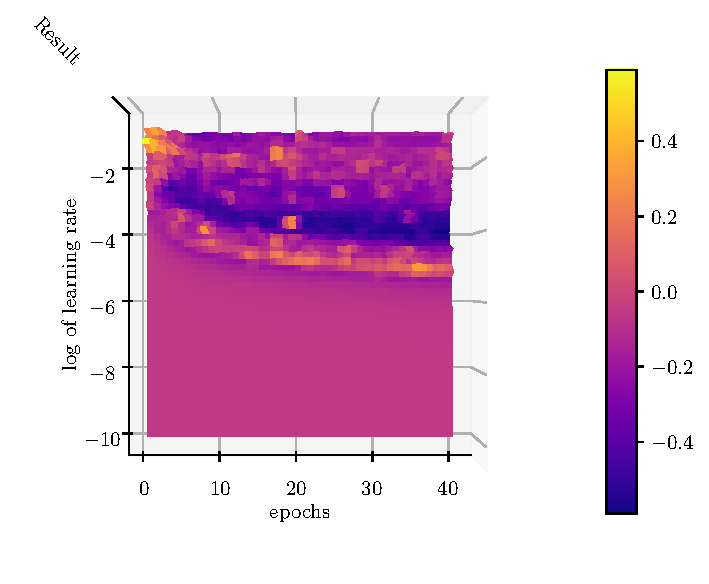
\includegraphics[width=0.48\textwidth]{figures/Results/Machine_learning/1000_evaluations/Network_above}
	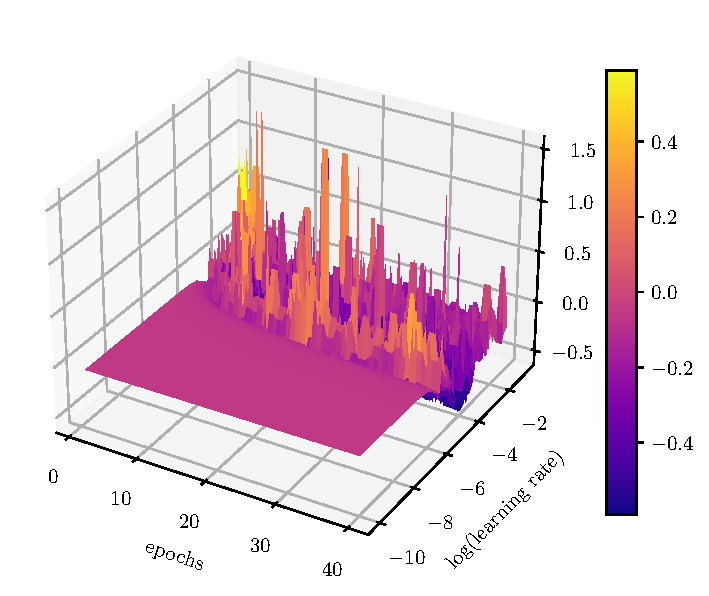
\includegraphics[width=0.48\textwidth]{figures/Results/Machine_learning/1000_evaluations/Network_normal}
	
	\caption{ 2-layer (with 30 neurons each) fully connected network evaluation on the diamonds dataset depending on the number of epochs and learning rate of the Adam optimizer. The result is plotted with $ log_{10}(\text{Result}) $ for better visualization. }
	\label{fig:analysis_model_training}
\end{figure}

In the plot in Figure \ref{fig:analysis_model_training}, for each epoch and learning rate, 100 different, equidistant values are sampled from the corresponding interval (linear sampling for epochs and log sampling for learning rate). All different combinations are evaluated leading to $ 100^2 = 10000 $ function evaluations. This took about 45 hours on a normal machine. Regarding the goal of hyperparameter optimization, this technique of trying all different combinations of distinct values is comparable to the grid search approach which is not very efficient. Although, the rough behavior of the machine learning model can be analyzed. The function is nearly constant for the learning rate between $ 10^{-6} $ and $ 10^{-10} $. This is caused by the Adam optimizer adjusting the weights of the network too slowly in order to minimize the error. In the other half of the domain (learning rate between $ 10^{-1} $ and $ 10^{-5} $), a blue region where the smallest errors are achieved can be observed. This is where the combination between epochs and the learning rate is very good for achieving good results. With this plot, a general observation can be made. However, it takes far too much time to analyze each problem with a plot like this. Additionally to the high effort, only the region of the minimum can be determined, not the optimal point itself. \newline

With this knowledge about the underlying function that has to be minimized, the behavior of the sparse grid can be analyzed. Figure \ref{fig:analysis_sparse_grid_with_machine_learning} depicts the generated grid colored corresponding to the function value for different adaptivity values and the number of grid points. Note that the scale of the learning rate is the one interpreted by the sparse grid. The actual scale is logarithmic between $ 10^{-10} $ for $ 0.0 $ and $ 10 ^{-1} $ for $ 1.0 $. 

\begin{figure}[H]
	\begin{subfigure}{\textwidth}
		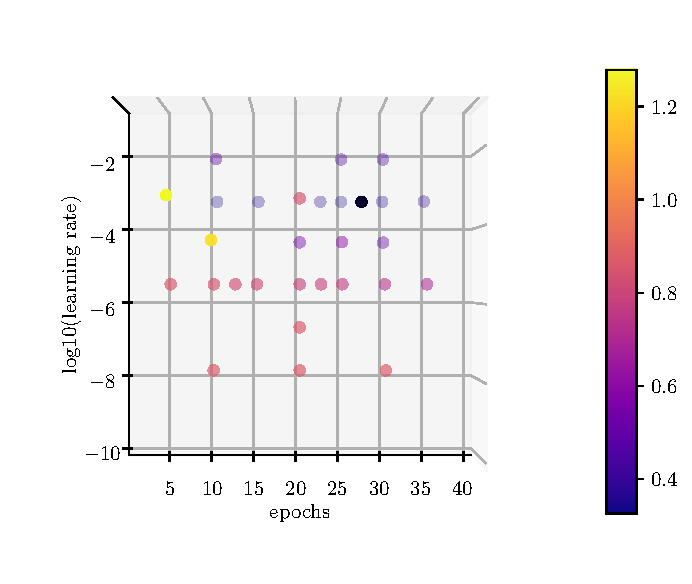
\includegraphics[width=0.48\textwidth]{figures/Results/Machine_learning/first_analysis/above_30_85}
		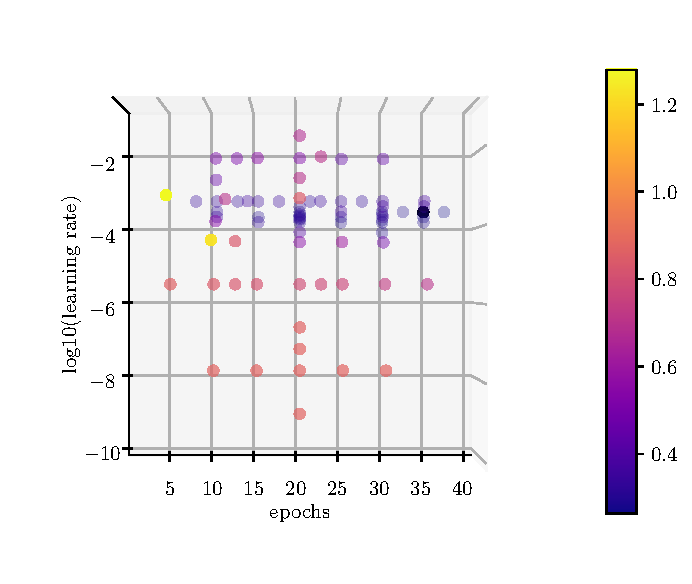
\includegraphics[width=0.48\textwidth]{figures/Results/Machine_learning/first_analysis/above_80_85}
		\caption{ Sparse grid generated with adaptivity parameter $ \gamma = 0.85 $ and number of grid points of 29 (left) and 77 (right). Most points are in the upper half for higher values of the learning rate. }
		\label{fig:analysis_sparse_grid_with_machine_learning_085}
	\end{subfigure}
	
	\begin{subfigure}{\textwidth}
		\includegraphics[width=0.48\textwidth]{figures/Results/Machine_learning/first_analysis/Above_30_5}
		\includegraphics[width=0.48\textwidth]{figures/Results/Machine_learning/first_analysis/Above_80_5}
		\caption{Sparse grid generated with adaptivity parameter $ \gamma = 0.5 $ and number of grid points of 29 (left) and 77 (right). Most points are in the upper right half for higher values of the learning rate and epochs between 25 and 30. }
		\label{fig:analysis_sparse_grid_with_machine_learning_05}
	\end{subfigure}

	\caption{ Analysis of sparse grid with machine learning evaluation for different adaptivity parameters ($ 0.85 $ \ref{fig:analysis_sparse_grid_with_machine_learning_085} and $ 0.5 $ \ref{fig:analysis_sparse_grid_with_machine_learning_05}), each with 29 and 77 grid points.}
	\label{fig:analysis_sparse_grid_with_machine_learning}
\end{figure}

In the first case with $ \gamma = 0.85 $, more grid points are generated in the upper half of the domain. A similar behavior can be observed for a higher number of grid points (\ref{fig:analysis_sparse_grid_with_machine_learning_085}, right). Especially in regions where the learning rate is about $ 0.0002 $ to $ 0.0003 $ (scale marked at $ 0.7 $), many grid points are refined. From the analysis in Figure \ref{fig:analysis_model_training}, there might be the optimal value. 

For a smaller adaptivity value of $ \gamma = 0.5 $, the sparse grid is much more adaptive as depicted in Figure \ref{fig:analysis_sparse_grid_with_machine_learning_05}. For both the number of grid points $ 50 $ and $ 100 $, the most refined part of the sparse grid is at the same region. One important thing to observe here is that with higher adaptivity, a lower number of grid points is necessary to find one candidate of the optimum value. On the other hand, with lower adaptivity, more grid points are needed to find a good minimal value. 

However, as shown in Table \ref{tab:analysis_sparse_grid_with_machine_learning_results}, the best value is found with the configuration $ \gamma = 0.85 $ and number of grid points of 100. This means that lower adaptivity leads to better results.

\begin{table}[H]
	\centering
	\caption{ Best hyperparameter configuration found by the sparse grid with different adaptivity parameters and number of grid points. The best result is found with $ \gamma = 0.85 $ and 77 grid points. }
	\label{tab:analysis_sparse_grid_with_machine_learning_results}
	\begin{tabular}{| c c | c c | c |} 
		\hline
		$ \gamma $ & N &  Epochs & Learning rate & Result \\
		\hline
%		0.85 & 29 & 27 & 0.0005623413251903491 & 0.3259957134723667 \\
%		0.85 & 77 & 35 & 0.00029427271762092817 & \textbf{0.26339022070169354} \\
%		0.5 & 29 & 26 & 0.00015399265260594922 & 0.26837945729494134 \\
%		0.5 & 77 & 26 & 0.00015399265260594922 & 0.2683794572949415 \\
		0.85 & 29 & 27 & 0.00056 & 0.32599 \\
		0.85 & 77 & 35 & 0.00029 & \textbf{0.26339} \\
		0.5 & 29 & 26 & 0.00015 & 0.26837 \\
		0.5 & 77 & 26 & 0.00015 & 0.26837 \\
		\hline
	\end{tabular}
\end{table}

The results shown in this table prove that too high adaptivity is not good for finding the smallest function value. However, when using higher adaptivity, the number of grid points has no big impact on finding the best solution in this case. This is because of the function shown in Figure \ref{fig:analysis_model_training}. In general, a higher adaptivity is good for finding a configuration faster. This can be useful in cases of hyperparameter optimization where not much time is available and a relatively good solution is enough. 

\subsection{Optimization on Sparse Grids}

By adding optimization methods like gradient descent or evolutionary algorithms, an even better approximation of the optimum might be found if enough grid points are available. If this number is too small then the interpolant is not precise enough and the solution of the optimizer is not the real optimum. One example is depicted in Figure \ref{fig:optimizers_network_visualization}. The steps of the normal gradient descent optimization algorithm are depicted and connected with arrows. In the background, the interpolated function is shown. The problem is the same as in Figure \ref{fig:analysis_model_training}. The degree of the B-splines on the grid is 2 and the sparse grid points are shown in white. 

\begin{figure}[H]
	\centering
	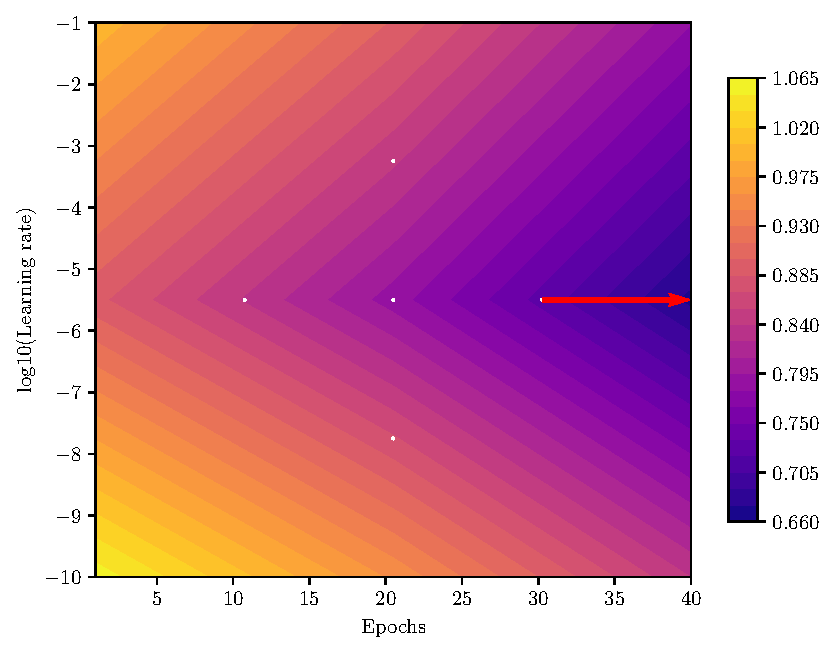
\includegraphics[width=0.49\textwidth]{figures/Results/Machine_learning/optimizer/Optimizers_visualization_ml_5}
	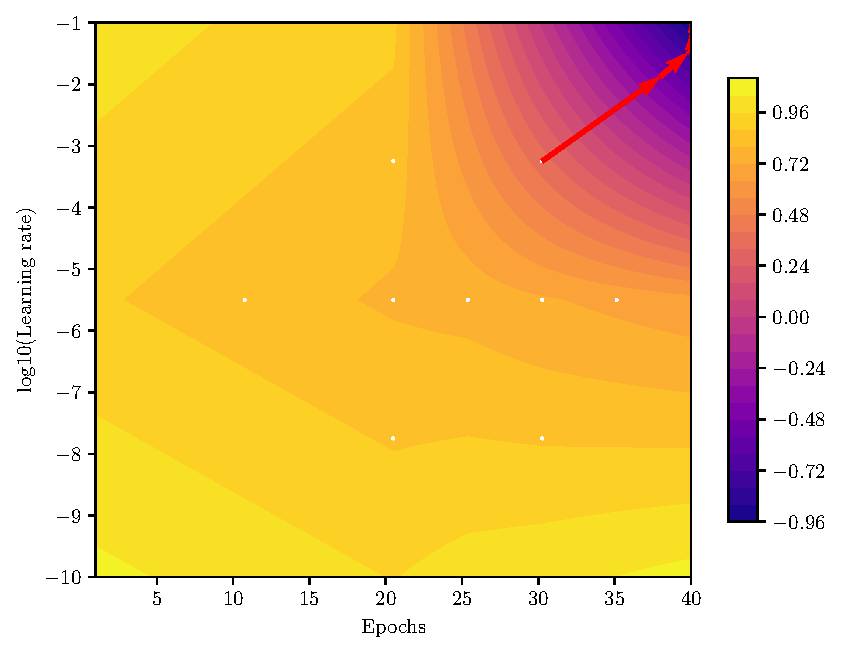
\includegraphics[width=0.49\textwidth]{figures/Results/Machine_learning/optimizer/Optimizers_visualization_ml_10}
	
	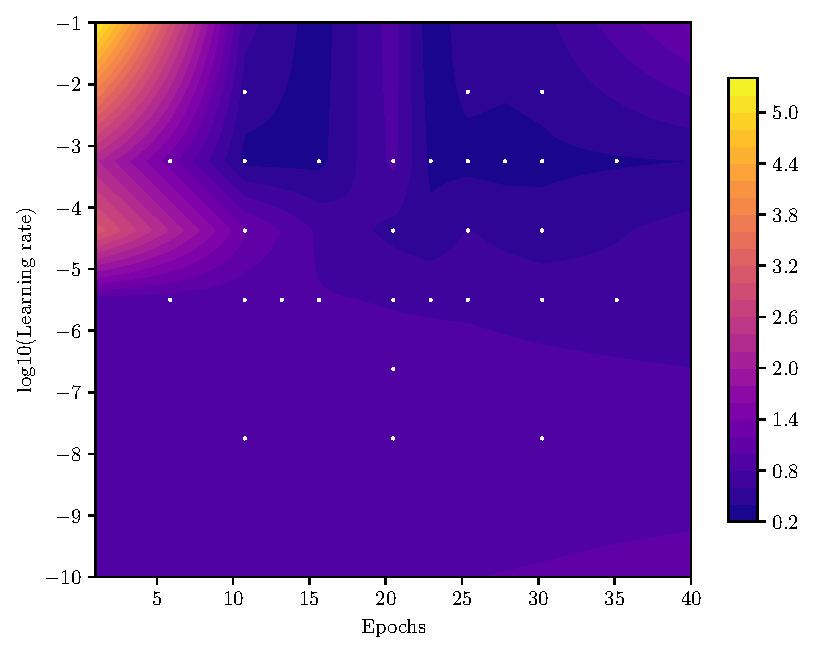
\includegraphics[width=0.49\textwidth]{figures/Results/Machine_learning/optimizer/Optimizers_visualization_ml_30}
	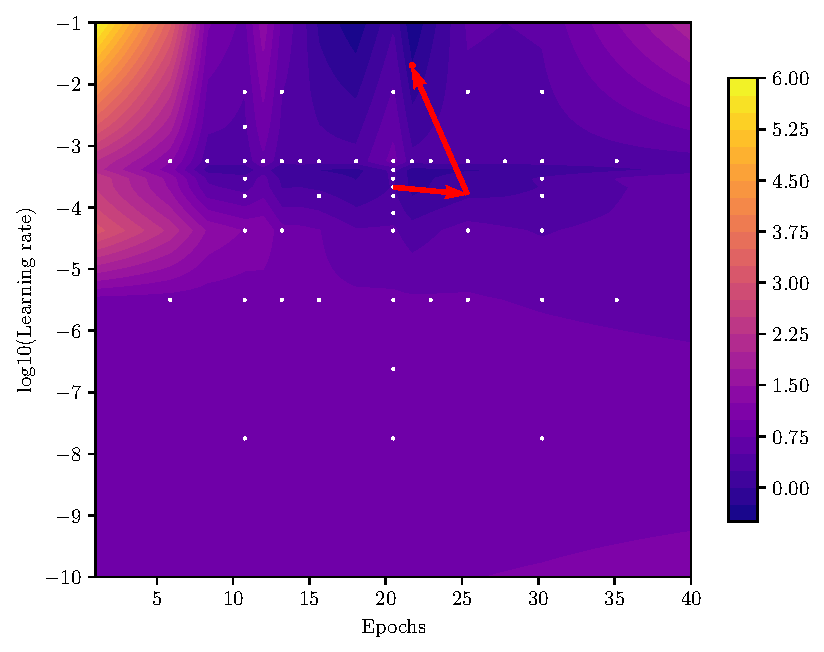
\includegraphics[width=0.49\textwidth]{figures/Results/Machine_learning/optimizer/Optimizers_visualization_ml_50}
	
	\caption{ Optimization steps of gradient descent algorithm for 5 (top left), 9 (top right), 29 (bottom left) and 49 (bottom right) grid points. In the background of each plot, the contour of the interpolated function is shown. The function evaluated is the same as depicted in Figure \ref{fig:analysis_model_training}. }
	\label{fig:optimizers_network_visualization}
\end{figure}

In Figure \ref{fig:optimizers_network_visualization}, the solution of the gradient descent optimization algorithm is analyzed with 5, 9, 29 and 49 grid points on the top left, top right, bottom left and bottom right, respectively. The minimal interpolated function values and the actual function evaluations can be seen in Table \ref{tab:results_opt_ml}.


\begin{table}[H]
	\caption{ Exact values for the optima found by the sparse grid points and the gradient descent algorithm. The values for $ x_{min}^{grid} $ are the configurations evaluated by the sparse grid during the generation and the coordinates in column $ x_{min}^{opt} $ are found by the optimizer. In bold, the best function values of the optimum found by the sparse grid and gradient descent algorithm, respectively. }
	\label{tab:results_opt_ml}
	\centering
	\begin{tabular}{| c c c c c c |} 
		\hline
		N & $ x_{min}^{grid} $ & $ f(x_{min}^{grid}) $ & $ x_{min}^{opt} $ & $ f(x_{min}^{opt}) $ & $ f_{interpolated}(x_{min}^{opt}) $ \\ 
		\hline
		5 & $ (30.25, 3.162*10^{-6}) $ & $ 0.729 $ & $ (40, 3.162*10^{-6}) $ & $ 0.668 $ & $ 0.670 $ \\ 
		9 & $ (30.25, 5.623*10^{-4}) $ & $ 0.353 $ & $ (40, 1*10^{-1}) $ & $ 1.257 $ & $ -0.950 $ \\ 
		29 & $ (27.81, 5.623*10^{-4}) $ & $ 0.326 $ & $ (27.81,5.623*10^{-4}) $ & $ \mathbf{0.326} $ & $ 0.326 $ \\ 
		49 & $ (20.5, 2.129*10^{-4}) $ & $ \mathbf{0.267} $ & $ (21.72,2.094*10^{-2}) $ & $ 0.524 $ & $ -0.247 $ \\ 
		\hline
	\end{tabular}
\end{table}

In the first case, the optimizer starts at the right grid points and makes one step towards the right boundary of the domain. In the top right case with 9 grid points, the solution of the optimizer is at the right top corner of the domain. With 29 basis points in the left lower case, the solution of the optimizer is the same as the grid point with the smallest evaluated function value and in the right lower plot, the optimizer first takes a step to the right and then a second step up to a higher learning rate. 

As illustrated in Table \ref{tab:results_opt_ml}, the optimizer does not always find an actual better solution. While the interpolated function value actually decreases, the evaluation of the network with the given configuration results in a higher value which is worse. This behavior is the same as in Figure \ref{fig:Optimizer_results} where both optimizers lead to a higher error than the smallest value found by the sparse grid. This is due to the small number of function evaluations made so far and the interpolant of the function being too inaccurate. Also the visual comparison of the interpolant plots in Figure \ref{fig:optimizers_network_visualization} and Figure \ref{fig:analysis_model_training} shows that there are still big differences. Nevertheless in the scope of this thesis, further increasing the number of grid points is infeasible because of the high costs of one single function evaluation which is the training and evaluation of a machine learning model. \newline

Note that the additional optimization is very cheap compared to generating the adaptive sparse grid because the algorithm uses the interpolated function and does not have to train and evaluate whole machine learning models. In Figure \ref{fig:Comparison_optimizers}, the different algorithms for optimization based on the sparse grid are compared. The same neural network with the same dataset is used for the comparison.


\begin{figure}[H]
	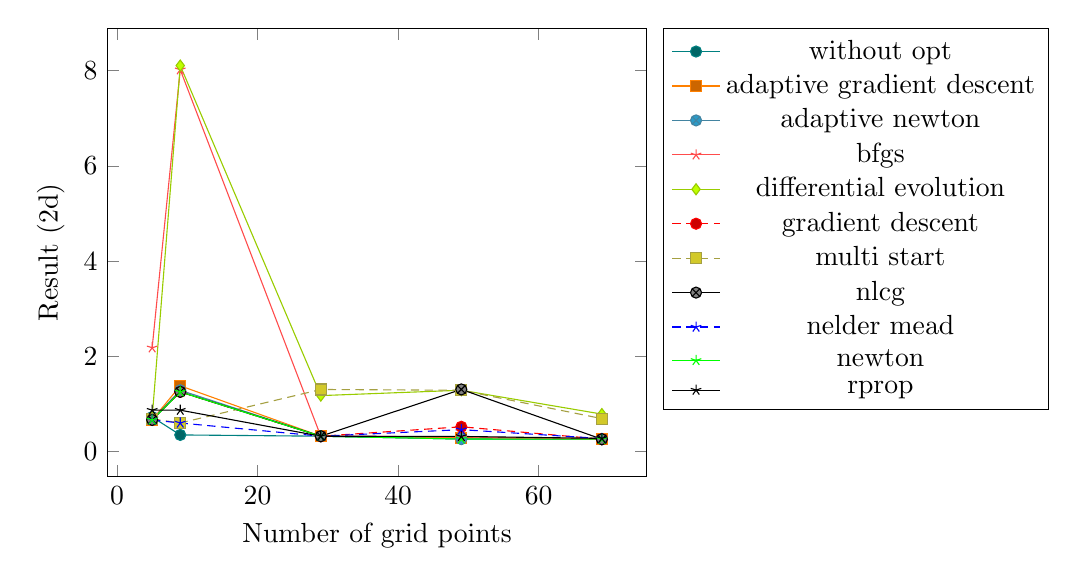
\begin{tikzpicture}
		\begin{axis}[
			xlabel = Number of grid points,
			ylabel = Result (2d),
			cycle list name=exotic,
			legend pos=outer north east,
			scale=1
			]
			
			\addplot coordinates
			{(5,0.7287221550941467)(9,0.3527909889817238)(29,0.32599571347236633)(49,0.2671877220273018)(69,0.2633902207016945)};
			
			\addplot coordinates 
			{(5,0.6684863269329071)(9,1.3836875557899475)(29,0.32599571347236633)(49,0.29520951211452484)(69,0.2633902207016945)};
			
			\addplot coordinates
			{(5,0.6684863269329071)(9,1.290485441684723)(29,0.32599571347236633)(49,0.2671877220273018)(69,0.2633902207016945)};
			
			\addplot coordinates 
			{(5,2.1821350157260895)(9,8.017291724681854)(29,0.32599571347236633)(49,0.3126538023352623)(69,0.2633902207016945)};
			
			\addplot coordinates 
			{(5,0.7181140184402466)(9,8.104115903377533)(29,1.1781185865402222)(49,1.290873944759369)(69,0.7903150916099548)};
			
			\addplot coordinates
			{(5,0.6684863269329071)(9,1.2569370865821838)(29,0.32599571347236633)(49,0.5238737538456917)(69,0.2633902207016945)};
			
			\addplot coordinates 
			{(5,0.6905131638050079)(9,0.6032524108886719)(29,1.3066118955612183)(49,1.2903412878513336)(69,0.6954652667045593)};
			
			\addplot coordinates
			{(5,0.6684863269329071)(9,1.2569370865821838)(29,0.32599571347236633)(49,1.3082255125045776)(69,0.2633902207016945)};
			
			\addplot coordinates 
			{(5,0.6684863269329071)(9,0.6032524108886719)(29,0.32599571347236633)(49,0.4634876996278763)(69,0.27645721286535263)};
			
			\addplot[green,mark=star] coordinates
			{(5,0.6684863269329071)(9,1.2569370865821838)(29,0.32599571347236633)(49,0.2671877220273018)(69,0.2633902207016945)};
			
			\addplot[black,mark=star] coordinates 
			{(5,0.872105598449707)(9,0.8723746538162231)(29,0.32599571347236633)(49,0.32110922783613205)(69,0.2806633412837982)};
			
			
			\legend{without opt, adaptive gradient descent, adaptive newton, bfgs, differential evolution, gradient descent, multi start, nlcg, nelder mead, newton, rprop}
			
		\end{axis}
	\end{tikzpicture}
\centering
	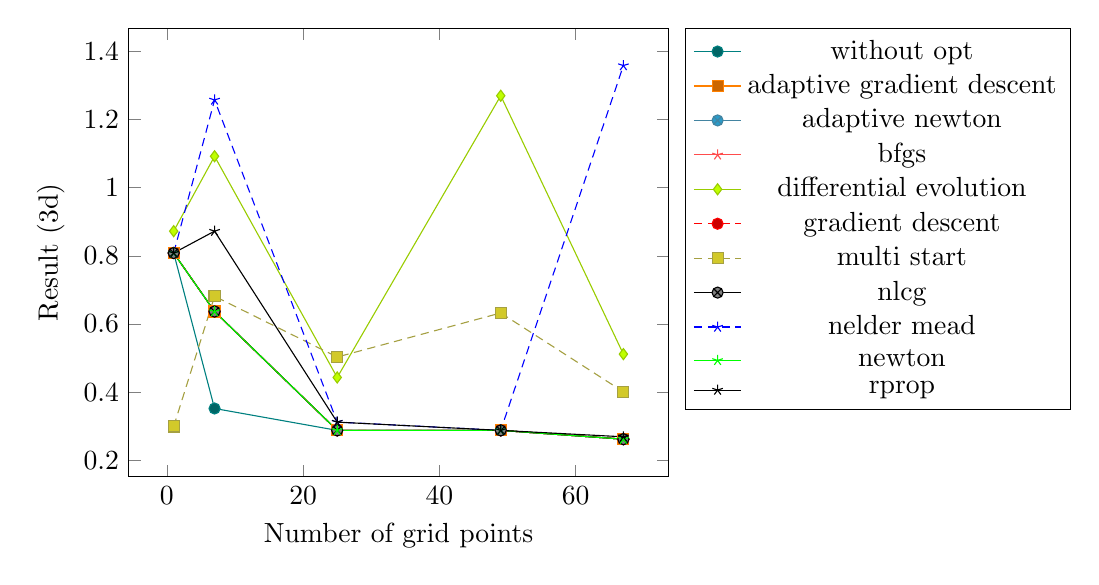
\begin{tikzpicture}
		\begin{axis}[
			xlabel = Number of grid points,
			ylabel = Result (3d),
			cycle list name=exotic,
			legend pos=outer north east,
			scale=1
			]
			
			\addplot coordinates
			{(1,0.8082304298877716)(7,0.3521949201822281)(25,0.2879640683531761)(49,0.2879640683531761)(67,0.26214249432086945)};
			
			\addplot coordinates 
			{(1,0.8082304298877716)(7,0.6366344541311264)(25,0.2879640683531761)(49,0.2879640683531761)(67,0.26214249432086945)};
			
			\addplot coordinates
			{(1,0.8082304298877716)(7,0.6366344541311264)(25,0.2879640683531761)(49,0.2879640683531761)(67,0.26214249432086945)};
			
			\addplot coordinates 
			{(1,0.8082304298877716)(7,0.6366344541311264)(25,0.2879640683531761)(49,0.2879640683531761)(67,0.26214249432086945)};
			
			\addplot coordinates
			{(1,0.8723749816417694)(7,1.0919488668441772)(25,0.44320355355739594)(49,1.269576072692871)(67,0.5115671902894974)};
			
			\addplot coordinates 
			{(1,0.8082304298877716)(7,0.6366344541311264)(25,0.2879640683531761)(49,0.2879640683531761)(67,0.26214249432086945)};
			
			\addplot coordinates
			{(1,0.2994298115372658)(7,0.6812499314546585)(25,0.503110408782959)(49,0.6323543787002563)(67,0.401133269071579)};
			
			\addplot coordinates 
			{(1,0.8082304298877716)(7,0.6366344541311264)(25,0.2879640683531761)(49,0.2879640683531761)(67,0.26214249432086945)};
			
			\addplot coordinates
			{(1,0.8082304298877716)(7,1.2571589648723602)(25,0.31235726177692413)(49,0.2879640683531761)(67,1.3579680025577545)};
			
			\addplot[green,mark=star] coordinates 
			{(1,0.8082304298877716)(7,0.6366344541311264)(25,0.2879640683531761)(49,0.2879640683531761)(67,0.26214249432086945)};
			
			\addplot[black,mark=star] coordinates
			{(1,0.8082304298877716)(7,0.8723750114440918)(25,0.31212611496448517)(49,0.2879640683531761)(67,0.2691311687231064)};
			
			\legend{without opt, adaptive gradient descent, adaptive newton, bfgs, differential evolution, gradient descent, multi start, nlcg, nelder mead, newton, rprop}
			
		\end{axis}
	\end{tikzpicture}
	\caption{ Comparison of optimization algorithms on the sparse grid with increasing number of grid points in two and three dimensions. Epochs, learning rate, and the batch size of a two-layer neural network on the diamonds dataset for regression are optimized. Result is the mean absolute percentage error.  }	
	\label{fig:Comparison_optimizers}
\end{figure}

For both cases, the solution found by the sparse grid without the optimization step decreases with increasing number of basis points. For the optimizers, this is not always the case. The resulting machine learning performance with the configuration found by the respective algorithm is even much worse than the one found by the sparse grid in some cases. In comparison to Figure \ref{fig:Optimizer_results}, we are only using a small number of grid points and get the same result in this situation. But further increasing the number of grid points is not feasible because of the high evaluation cost of the neural network. \newline

One thing that has to be taken into consideration is that e.g. the epochs hyperparameter is not continuous. The values for the number of epochs are always integers converted with \textit{int()}. This means that all values in the interval $ [x, x+1] $ for any $ x \in \mathbb{N} $ are interpreted as the smaller integer $ x $. This means that there are regions in the interval that have the exact same function value because they are evaluated with the same configuration. This fact might impact the behavior of a gradient-based optimizer. If the function values in an interval are exactly the same then the gradient is zero in this interval. This would make it impossible to find the real optimum if the optimizer gets stuck. In the experiment shown in Figure \ref{fig:optimizer_categorical_hyperparams}, an extreme example is tried out. We use two hyperparameters with three distinct values each. The first one is the batch size with values from $ {100, 400, 2000} $ and the second one is epochs taking values from $ {1, 5, 13} $. In two dimensions, nine different configurations are then possible. We used B-splines of degree 0 and a regular sparse grid with the smallest adaptivity possible. As the machine learning model being evaluated, we took a 2-layer network with 30 neurons each and a learning rate of $ 10^{-5} $. As dataset, the diamonds regression set is used.

\begin{figure}[H]
	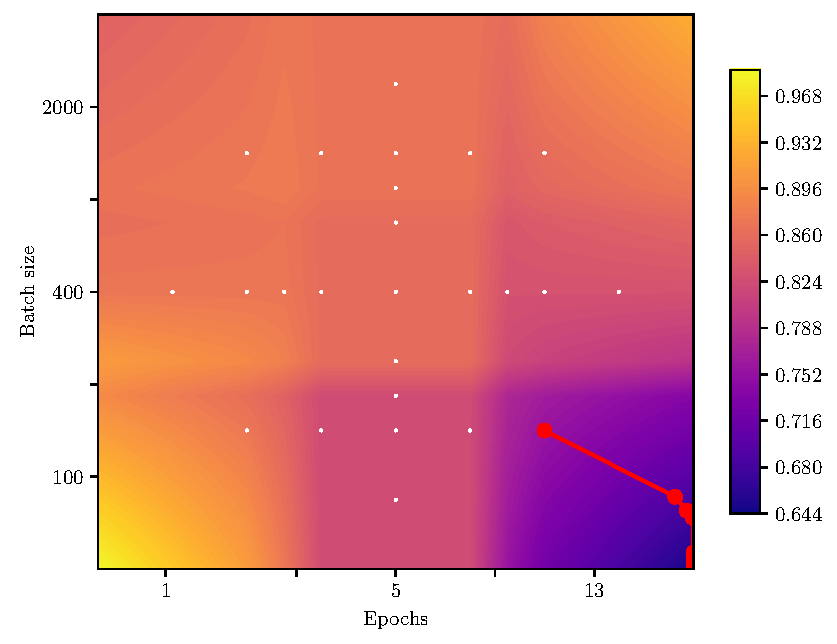
\includegraphics[width=0.48\textwidth]{figures/Results/Machine_learning/optimizer/categorical_hyperpar/Categorical_hyppar_28}
	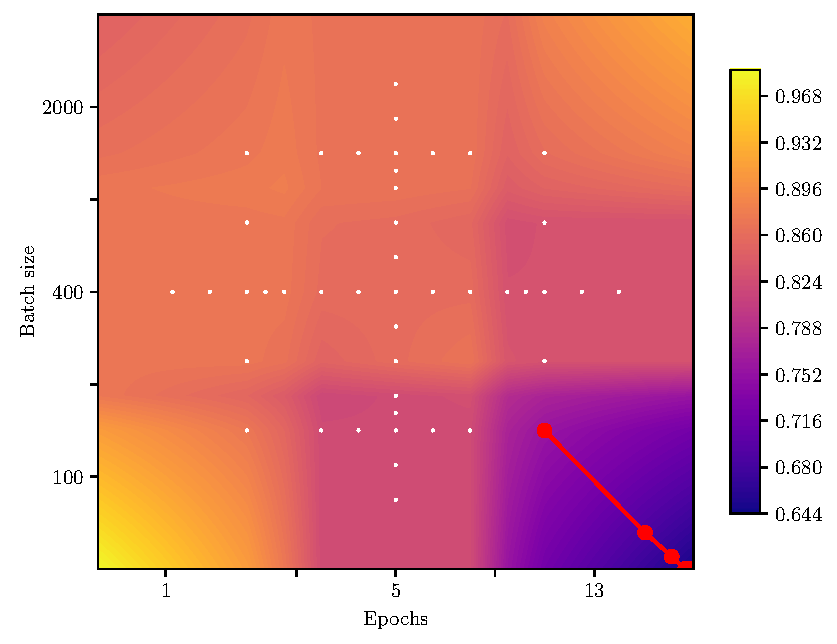
\includegraphics[width=0.48\textwidth]{figures/Results/Machine_learning/optimizer/categorical_hyperpar/Categorical_hyppar_48}
	
	
	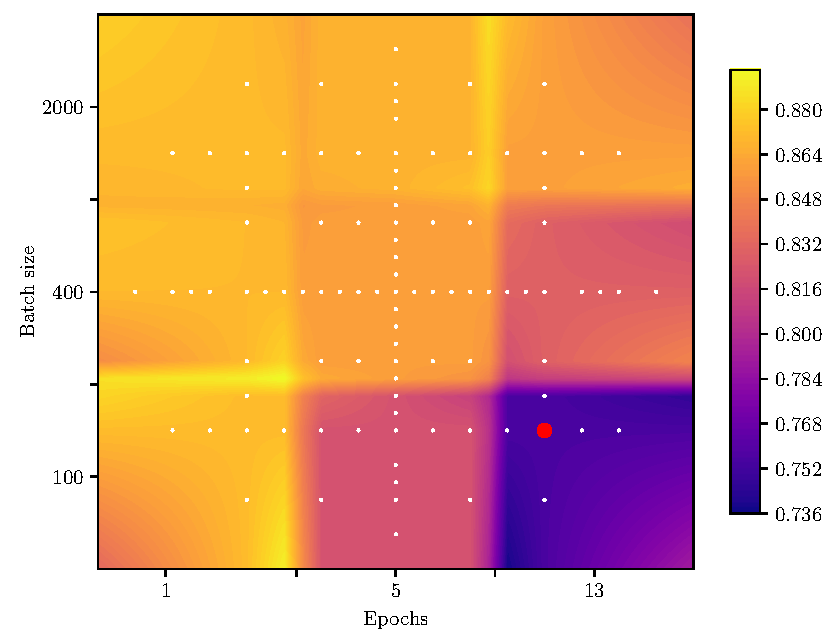
\includegraphics[width=0.48\textwidth]{figures/Results/Machine_learning/optimizer/categorical_hyperpar/Categorical_hyppar_98}
	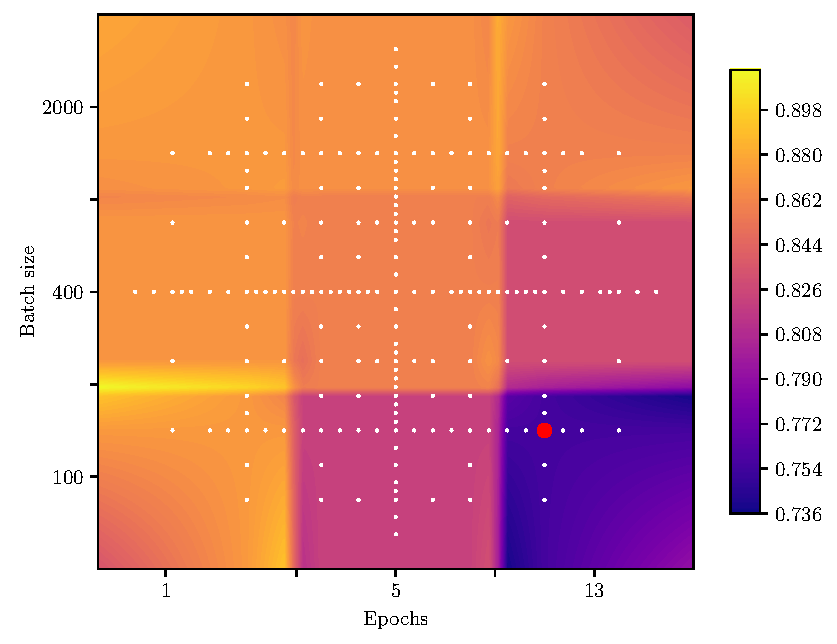
\includegraphics[width=0.48\textwidth]{figures/Results/Machine_learning/optimizer/categorical_hyperpar/Categorical_hyppar_198}
	
	\caption{ Sparse grid optimization with the interpolated function in the background, the white grid points, and the optimizer steps in red. Four different budgets are used (30: top left, 50: top right, 100: bottom left, 200: bottom right. Only three different configurations with values for batch size from $ {100, 400, 2000} $ and values for epochs from $ {1, 5, 13} $. }
	\label{fig:optimizer_categorical_hyperparams}
\end{figure}

In Figure \ref{fig:optimizer_categorical_hyperparams}, four different budgets (30, 50, 100, 200) which are shown top left, top right, bottom left and bottom right, respectively, are depicted. In each case, the interpolated function is shown in the background with the grid points from the sparse grid. In red, the steps of the gradient descent optimizer are shown. \newline 

We can observe one tendency. The more grid points are used, the more clear it gets that there are 9 different configurations and corresponding function values. For the first two cases in the top, the gradient descent still makes steps towards the bottom right corner of the domain. The interpolated function also still looks smooth. In the other two cases with a budget of 100 and 200, the optimizer does not take any steps because the grid points located next to the one with the smallest value also have the same smallest value. \newline 

Now in this case with only 9 distinct values, the sparse grid with its optimizer is finding the global optimum. But in other cases where there are more distinct configurations, this might lead to the optimizer not finding the global optimum. \newline


We can conclude that the use of any optimizer is not very promising for finding an improved solution in our case. However, we will still use a local and global optimizer because it is very cheap compared to the sparse grid generation and in some cases, the solution is improved. The resulting configuration returned by the algorithm will just be the best of the three alternatives. \newline


\section{Comparison with Grid-, Random Search and Bayesian Optimization}

Now with the sparse grid search being analyzed with defined functions and a small neural network, this algorithm will be compared to the already existing optimization methods presented in Chapter \ref{chapter:theoretical_background}. We will always compare the algorithms depending on some given budget. This is the upper bound for the number of function evaluations the algorithm is allowed to make. For the grid search, this budget is always $ n^d $ where $ d $ is the number of hyperparameters or dimension of the problem. Therefore, $ n $ different values are taken for each hyperparameter. On the other hand, for the sparse grid search, the highest number of grid points is $ budget - 2 $ because we have to evaluate the point of the local and global optimization for comparison. \newline 

\subsection{Two-dimensional Experiment of Regression with Small Neural Network}

The first experiment is using a two-layer neural network with 40 neurons in each layer. A batch size of 100 is used and as datasets, 4 different tasks from OpenML are taken. Table \ref{tab:datasets_first_experiment} gives an overview of the datasets. 

\begin{table}[H]
	\centering
	\caption{ Overview over the datasets used for the first comparison of the optimization algorithms. They are all available on OpenML \cite{OpenML2013}. }
	\label{tab:datasets_first_experiment}
	\begin{tabular}{| c | c | c | c |} 
		\hline
		 & \multicolumn{2}{c|}{Number of features} &   \\
		 Dataset& numeric & categorical & Number of instances  \\
		 \hline
		 diamonds & 7 & 3 & 53940  \\
		 house\_16H & 17 & 0 & 22784  \\
		 sensory & 11 & 1 & 576  \\
		 house\_sales & 16 & 2 & 21613  \\
		 Brazilian\_houses & 9 & 3 & 10692  \\
		\hline
	\end{tabular}
\end{table}

All the categorical features are transformed with one hot encoding and the numeric as well as the target values are scaled using the \textit{StandardScaler} from the \textit{scikit-learn} library \cite{scikit-learn}. Both transformers are trained on the training set and used for both training and test set. We used 2-fold cross-validation with the mean absolute percentage error as the metric. Before each run, the seeds for getting the random values are reset. This is necessary because the evaluation of the neural network with a specific configuration should always return the same value. For the B-splines on the sparse grid, we use a degree of 2 and the grid is generated with an adaptivity value of  $ 0.85 $. Two hyperparameters, the number of epochs and the learning rate for the neural network's optimizer, are optimized. The first one is linear from 1 to 40 and the second hyperparameter is logarithmic from $ 10^{-9} $ and $ 10^{-1} $. The resulting performance can be seen in Figure \ref{fig:result_first_comparison}. 

\begin{figure}[H]
	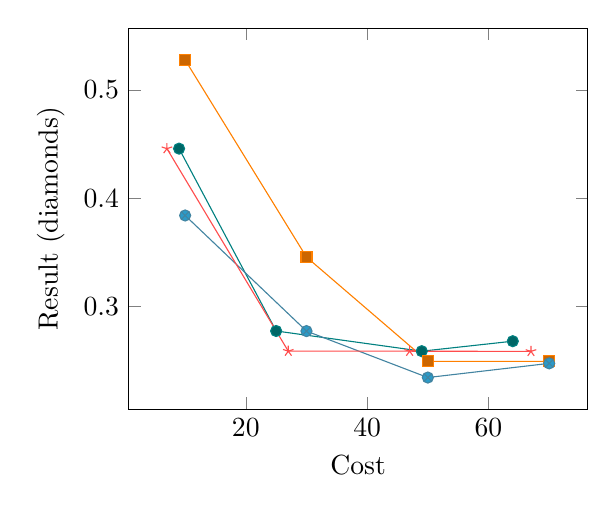
\begin{tikzpicture}
		\begin{axis}[
			xlabel = Cost,
			ylabel = Result (diamonds),
			cycle list name=exotic,
			legend pos=outer north east,
			scale=0.85
			]
			
			\addplot coordinates
			{(9,0.44587014615535736)(25,0.2773677632212639)(49,0.25869983434677124)(64,0.2679326832294464)};
			
			\addplot coordinates 
			{(10,0.5277889221906662)(30,0.34567804634571075)(50,0.2493194043636322)(70,0.2493194043636322)};
			
			\addplot coordinates
			{(10,0.3841075301170349)(30,0.27727870643138885)(50,0.23435243219137192)(70,0.24744291603565216)};
			
			\addplot coordinates 
			{(7,0.44587014615535736)(27,0.25871288776397705)(47,0.25869983434677124)(67,0.2585172727704048)};
			
			
		\end{axis}
	\end{tikzpicture}
	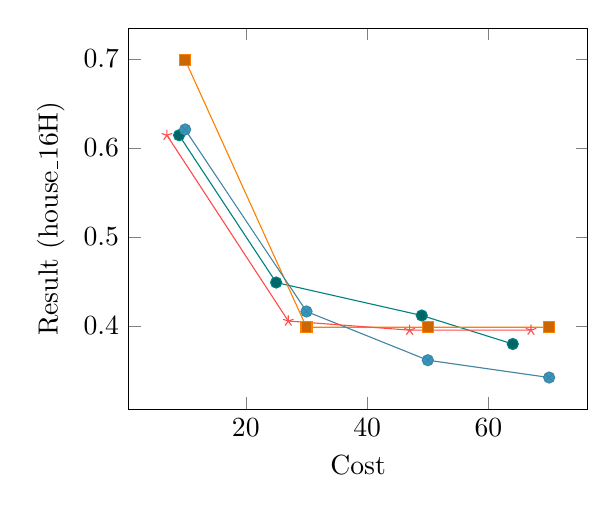
\begin{tikzpicture}
		\begin{axis}[
			xlabel = Cost,
			ylabel = Result (house\_16H),
			cycle list name=exotic,
			legend pos=outer north east,
			scale=0.85
			]
			
			\addplot coordinates
			{(9,0.6142911016941071)(25,0.44890759885311127)(49,0.4118947982788086)(64,0.3798752874135971)};
			
			\addplot coordinates 
			{(10,0.6987867951393127)(30,0.39865100383758545)(50,0.39865100383758545)(70,0.39865100383758545)};
			
			\addplot coordinates
			{(10,0.6207705140113831)(30,0.41639772057533264)(50,0.36166810989379883)(70,0.3422168046236038)};
			
			\addplot coordinates 
			{(7,0.6142911016941071)(27,0.4056653678417206)(47,0.39544127881526947)(67,0.39544127881526947)};
		
		\end{axis}
	\end{tikzpicture}
	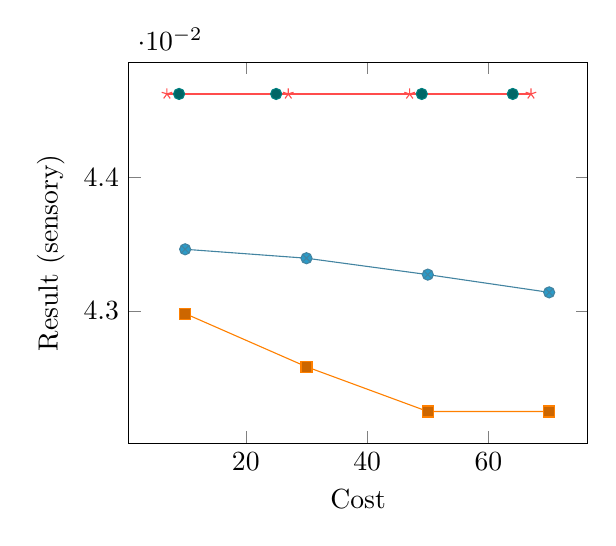
\begin{tikzpicture}
		\begin{axis}[
			xlabel = Cost,
			ylabel = Result (sensory),
			cycle list name=exotic,
			legend pos=outer north east,
			scale=0.85
			]
			
			\addplot coordinates
			{(9,0.04462818056344986)(25,0.04462808556854725)(49,0.04462808184325695)(64,0.04462808184325695)};
			
			\addplot coordinates 
			{(10,0.04297909699380398)(30,0.04257974028587341)(50,0.042243996635079384)(70,0.042243996635079384)};
			
			\addplot coordinates
			{(10,0.04346185550093651)(30,0.04339478723704815)(50,0.043271640315651894)(70,0.04313840717077255)};
			
			\addplot coordinates 
			{(7,0.04462807811796665)(27,0.04462807811796665)(47,0.04462807811796665)(67,0.04462807811796665)};
			
			
			
		\end{axis}
	\end{tikzpicture}
	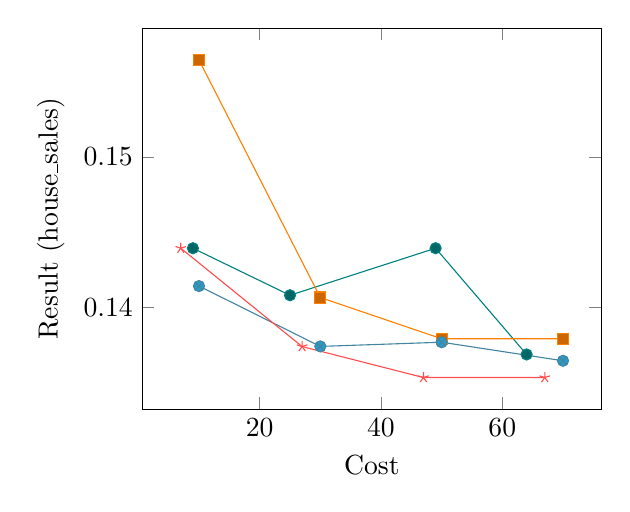
\begin{tikzpicture}
		\begin{axis}[
			xlabel = Cost,
			ylabel = Result (house\_sales),
			cycle list name=exotic,
			legend pos=outer north east,
			scale=0.85
			]
			
			\addplot coordinates
			{(9,0.14392731338739395)(25,0.14080144464969635)(49,0.14392731338739395)(64,0.13686956465244293)};
			
			\addplot coordinates 
			{(10,0.15643399953842163)(30,0.14065127074718475)(50,0.13791099935770035)(70,0.13791099935770035)};
			
			\addplot coordinates
			{(10,0.1414126306772232)(30,0.13740301132202148)(50,0.13768181949853897)(70,0.13644825667142868)};
			
			\addplot coordinates 
			{(7,0.14392731338739395)(27,0.13739430904388428)(47,0.13533496856689453)(67,0.13533496856689453)};
			
		\end{axis}
	\end{tikzpicture}
	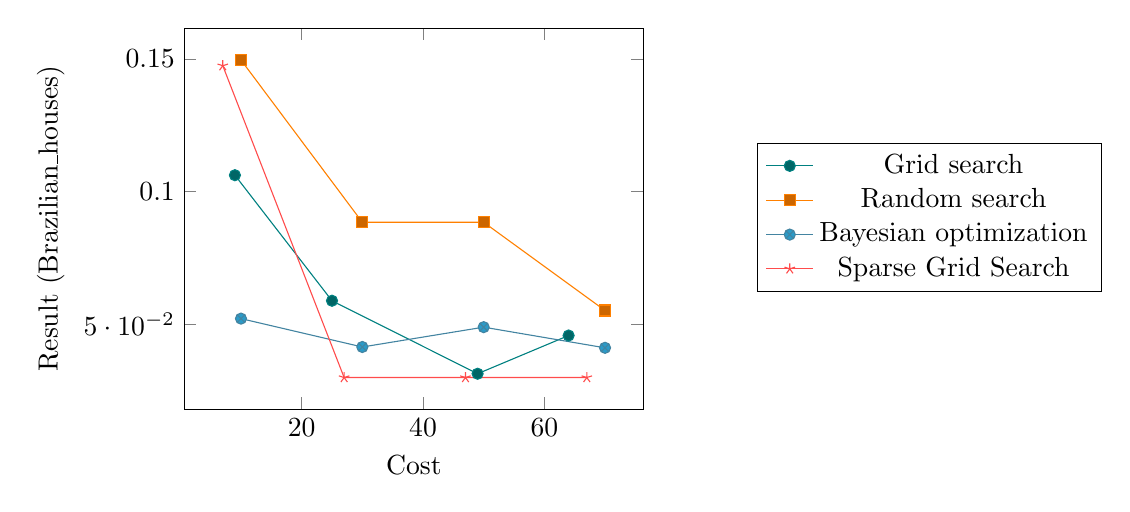
\begin{tikzpicture}
		\begin{axis}[
			xlabel = Cost,
			ylabel = Result (Brazilian\_houses),
			cycle list name=exotic,
			legend style={at={(2,0.7)}},
			scale=0.85
			]
			
			\addplot coordinates
			{(9,0.10614052042365074)(25,0.05877404101192951)(49,0.031237424351274967)(64,0.045658400282263756)};
			
			\addplot coordinates 
			{(10,0.14960936456918716)(30,0.0883832648396492)(50,0.0883832648396492)(70,0.055092256516218185)};
			
			\addplot coordinates
			{(10,0.052035532891750336)(30,0.04132956638932228)(50,0.04881274700164795)(70,0.04101819172501564)};
			
			\addplot coordinates 
			{(7,0.14743999391794205)(27,0.029803195036947727)(47,0.029803195036947727)(67,0.029803195036947727)};
			
			\legend{Grid search, Random search, Bayesian optimization, Sparse Grid Search}
			
		\end{axis}
	\end{tikzpicture}
	\caption{ Comparison of grid-, random search, bayesian optimization and sparse grid search for the datasets shown in Table \ref{tab:datasets_first_experiment}. Two hyperparameters, epochs and learning rate of the neural network's optimizer, were optimized. }	
	\label{fig:result_first_comparison}
\end{figure}

It can be seen that in almost all cases, the result is decreasing with increasing cost. For the house\_sales and Brazilian\_houses datasets, the sparse grid optimization is performing best for a cost which is higher than 20. For the sensory dataset, all four optimization algorithms already get very good results with small costs. This is due to the small number of data entries. This is not representative of general behavior. When comparing the normal grid search and the sparse grid optimization, the second one performs better in most cases. Figure \ref{fig:Comparison_visualization} shows the behavior for the house\_sales dataset and an upper bound of 10, 30, and 50 for the cost.

\begin{figure}[H]
	\begin{subfigure}{\textwidth}
		\centering
		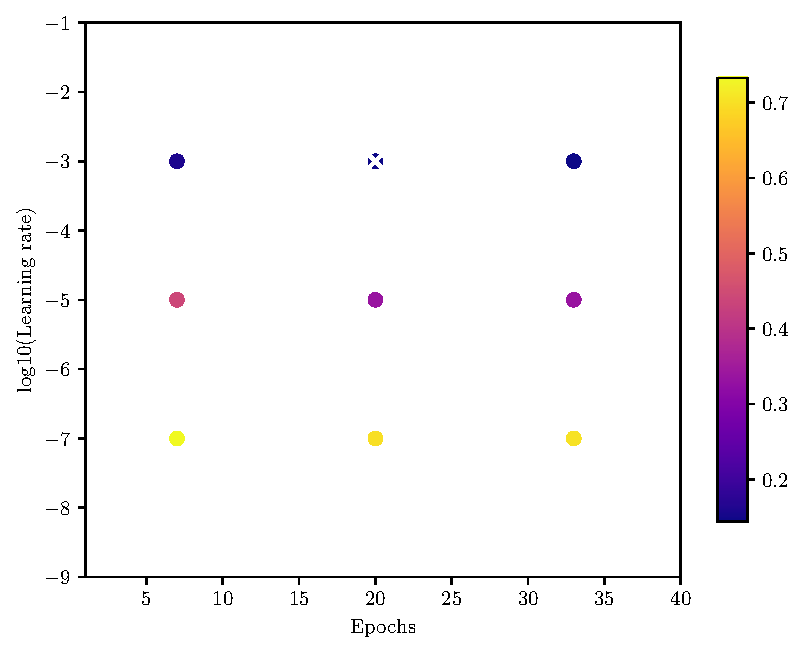
\includegraphics[width=0.31\textwidth]{figures/Results/First_comparison/Grid10}
		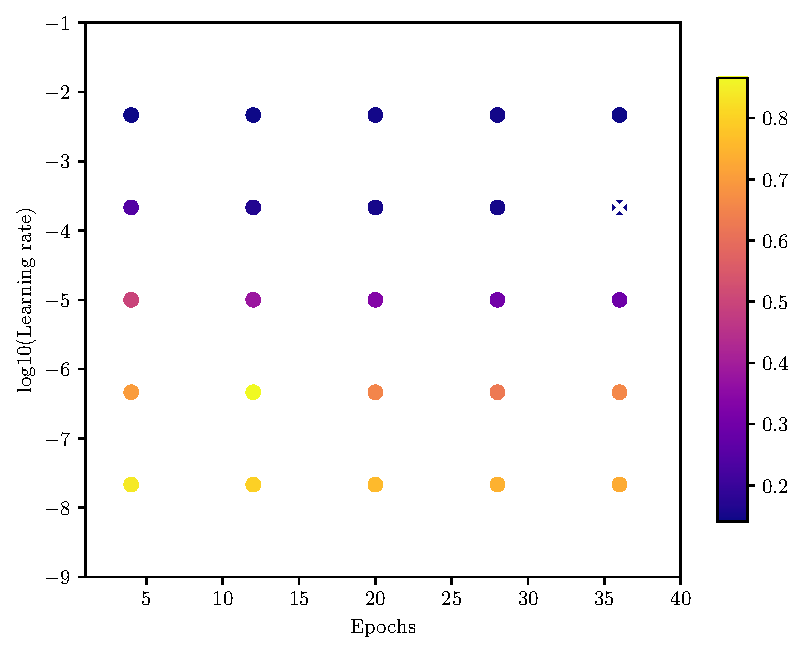
\includegraphics[width=0.31\textwidth]{figures/Results/First_comparison/Grid30}
		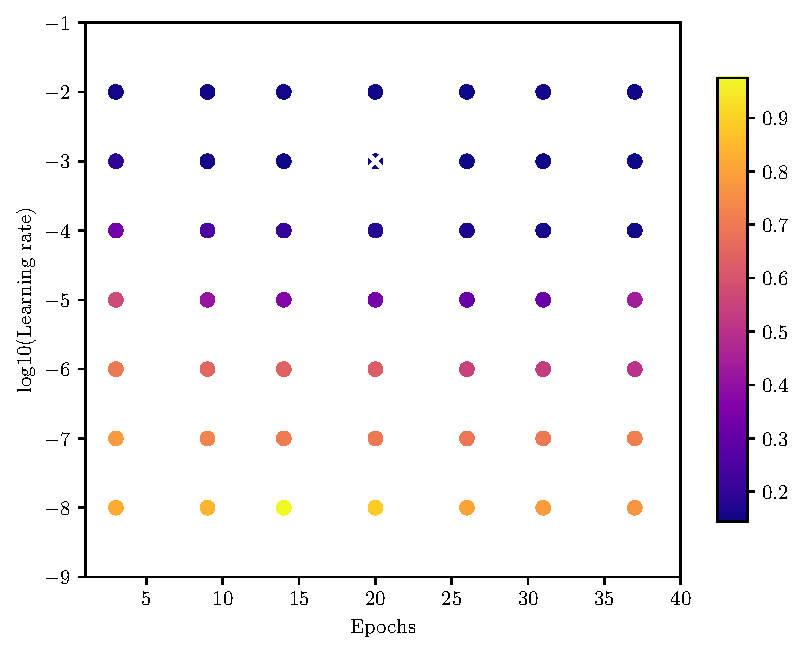
\includegraphics[width=0.31\textwidth]{figures/Results/First_comparison/Grid50}
		\caption{ Grid search with 9 (left, $f(x_{opt}) = 0.14393$), 25 (center, $f(x_{opt}) = 0.14080$), and 49 (right, $f(x_{opt}) = 0.14393$) grid points.}
		\label{fig:first_comparison_grid_search}
	\end{subfigure}
	\begin{subfigure}{\textwidth}
		\centering
		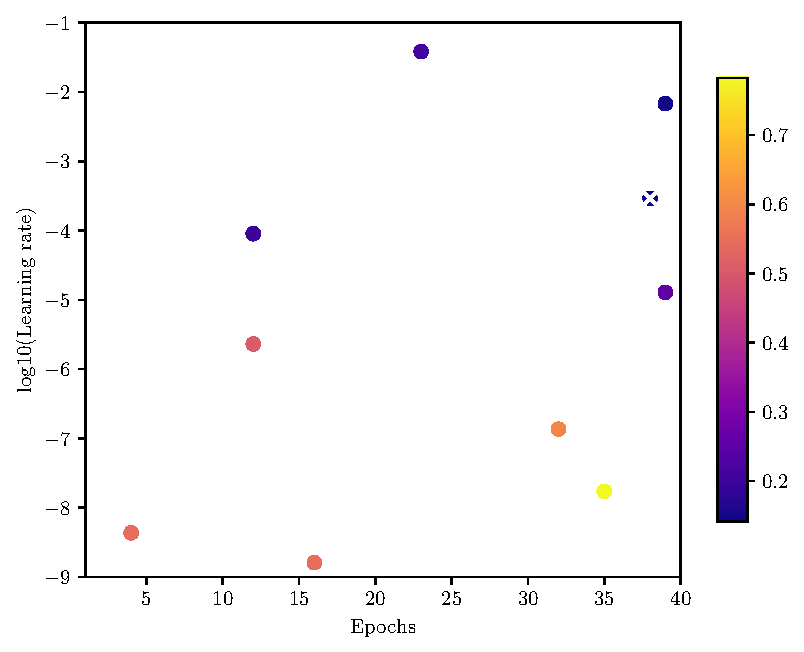
\includegraphics[width=0.31\textwidth]{figures/Results/First_comparison/Random10}
		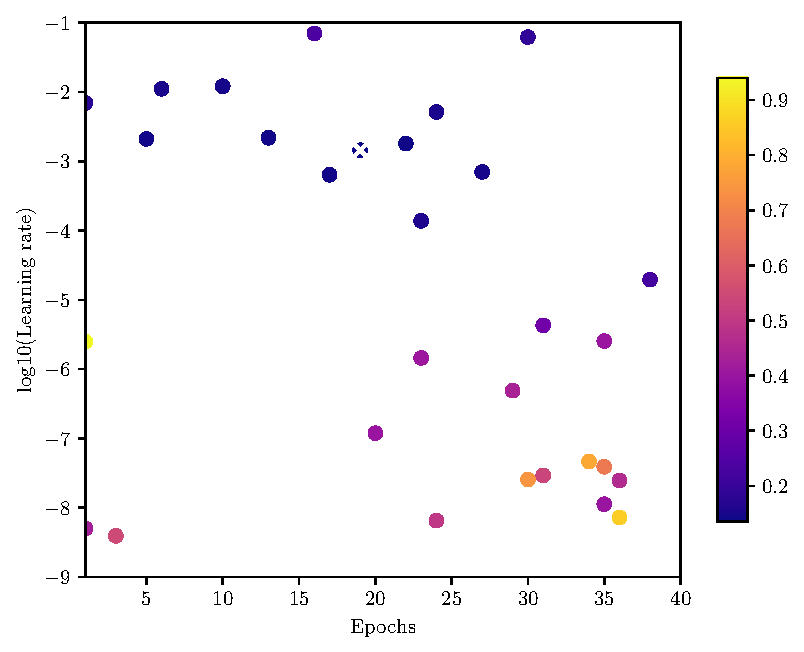
\includegraphics[width=0.31\textwidth]{figures/Results/First_comparison/Random30}
		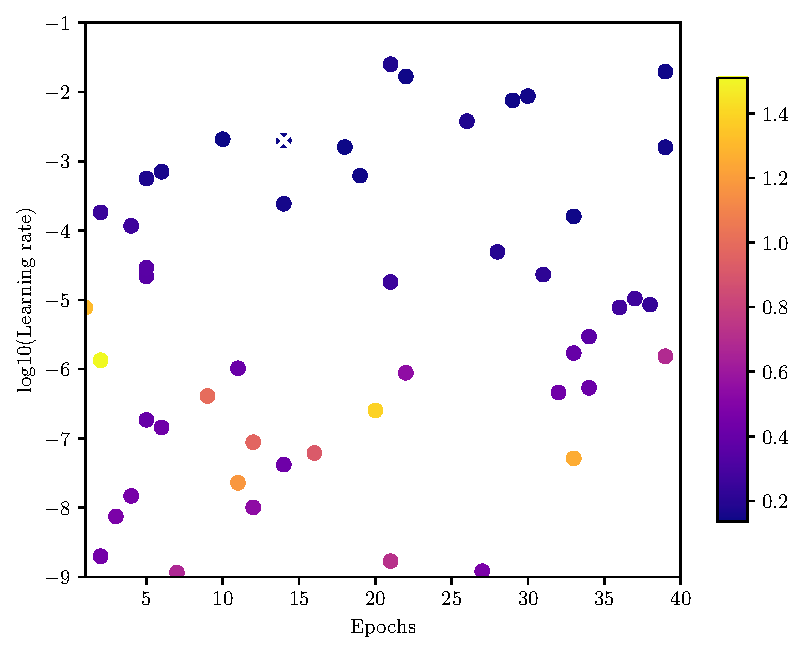
\includegraphics[width=0.31\textwidth]{figures/Results/First_comparison/Random50}
		\caption{ Random search with 10 (left, $f(x_{opt}) = 0.14141$), 30 (center, $f(x_{opt}) = 0.13526$), and 50 (right, $f(x_{opt}) = 0.13619$) samples. }
		\label{fig:first_comparison_random_search}
	\end{subfigure}
	\begin{subfigure}{\textwidth}
		\centering
		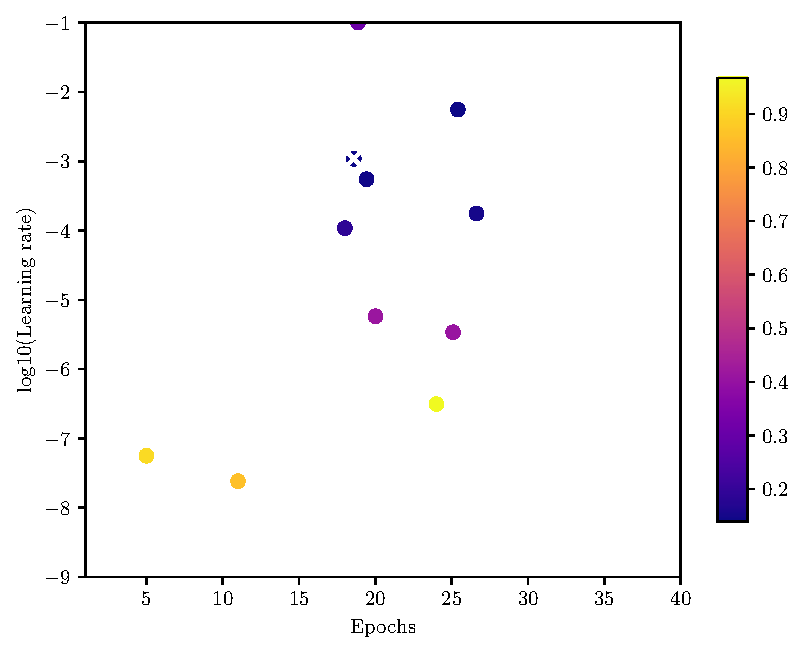
\includegraphics[width=0.31\textwidth]{figures/Results/First_comparison/Bayesian10}
		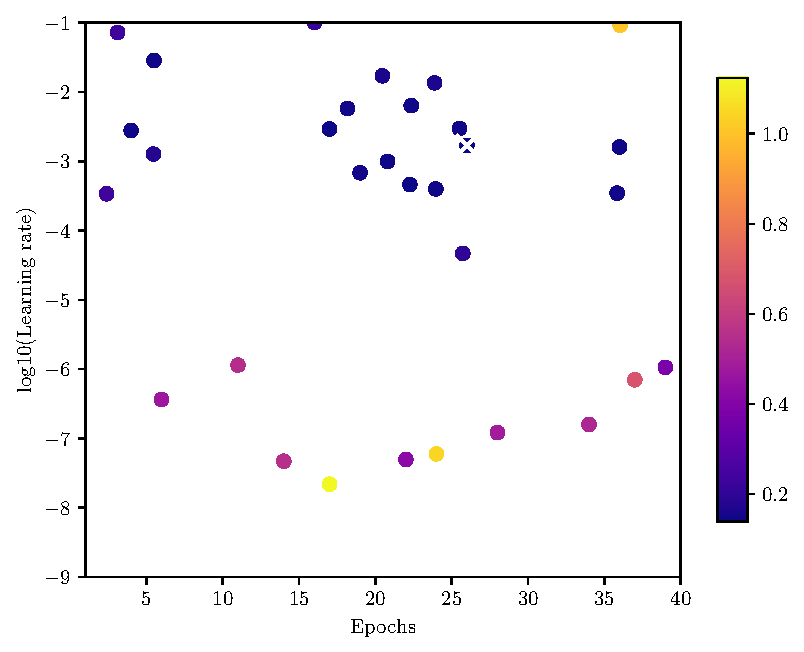
\includegraphics[width=0.31\textwidth]{figures/Results/First_comparison/Bayesian30}
		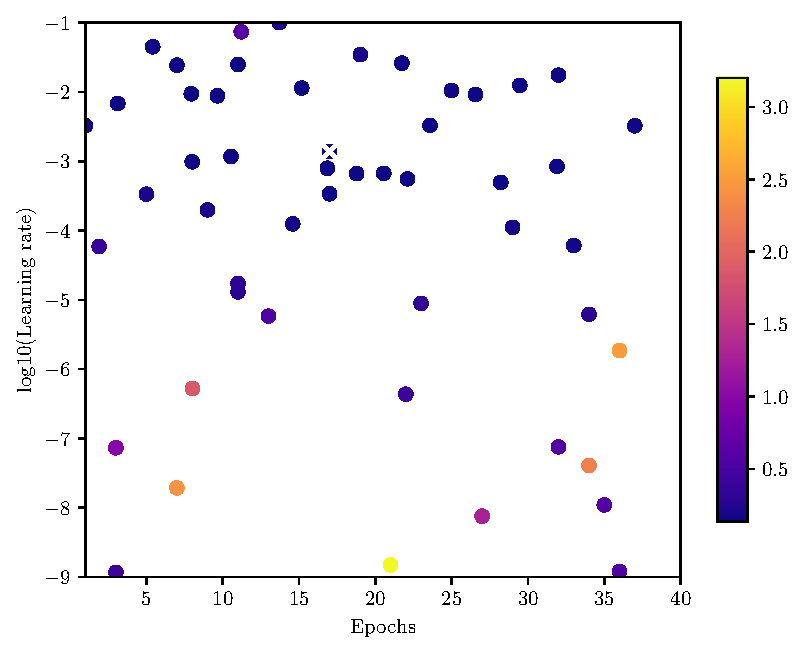
\includegraphics[width=0.31\textwidth]{figures/Results/First_comparison/Bayesian50}
		\caption{ Bayesian Optimization with 10 (left, $f(x_{opt}) = 0.13926$), 30 (center, $f(x_{opt}) = 0.13877$), and 50 (right, $f(x_{opt}) = 0.13542$) samples. }
		%\caption{ Sparse grid optimization... performance of \textbf{0.14393} (left), \textbf{0.13739} (center), and \textbf{0.13533} (right)  }
		\label{fig:first_comparison_bayesian_optimization}
	\end{subfigure}
	\begin{subfigure}{\textwidth}
		\centering
		\includegraphics[width=0.31\textwidth]{figures/Results/First_comparison/Sparse8}
		\includegraphics[width=0.31\textwidth]{figures/Results/First_comparison/Sparse28}
		\includegraphics[width=0.31\textwidth]{figures/Results/First_comparison/Sparse48}
		\caption{ Sparse grid optimization with 5 (left, $f(x_{opt}) = 0.14393$), 25 (center, $f(x_{opt}) = 0.13739$), and 45 (right, $f(x_{opt}) = 0.13533$) grid points. }
		\label{fig:first_comparison_sparse_optimization}
	\end{subfigure}
	
	\caption{ Comparison of the grids generated for the house\_sales dataset. The best configuration found $ x_{opt} $ is marked with a white cross.}
	\label{fig:Comparison_visualization}
\end{figure}

The big difference between grid search and sparse grid optimization is the adaptivity and the location of grid points. In Figure \ref{fig:Comparison_visualization}, this can be seen very clearly. While the grid generated for the grid search (see Figure \ref{fig:first_comparison_grid_search}) is very homogeneous and spread over the whole domain, the grid points are more gathered for the sparse grid optimization (see Figure \ref{fig:first_comparison_sparse_optimization}). For these upper bounds for the cost and for this dataset, the sparse grid optimization finds configurations with a bit better performance.


\subsection{Three- and Five-dimensional Experiments of Regression with Small Neural Network}

While the two-dimensional case is good for the visualization of the approaches, one is often interested in the optimization of more hyperparameters. In the following, we will focus again on regression problems, but this time we will include the batch size, the number of neural layers, and the number of neurons per layer in the hyperparameter space. \newline 

For the three-dimensional case, we first use the same network with fixed architecture again, consisting of 2 layers with 40 neurons each. The hyperparameter space consists of the epochs, the batch size and the learning rate of the neural network. The first two are linear integers from 1 to 40 for the epochs and the batch size has 100 and 2050 as bounds. The learning rate is again logarithmic from $ 10^{-9} $ to $ 10^{-1} $. We used the three datasets house\_16H, house\_sales, and Brazilian\_houses (see Table \ref{tab:datasets_first_experiment}). The resulting performance can be seen in Figure \ref{fig:result_second_comparison_dim3}. 


\begin{figure}[H]
	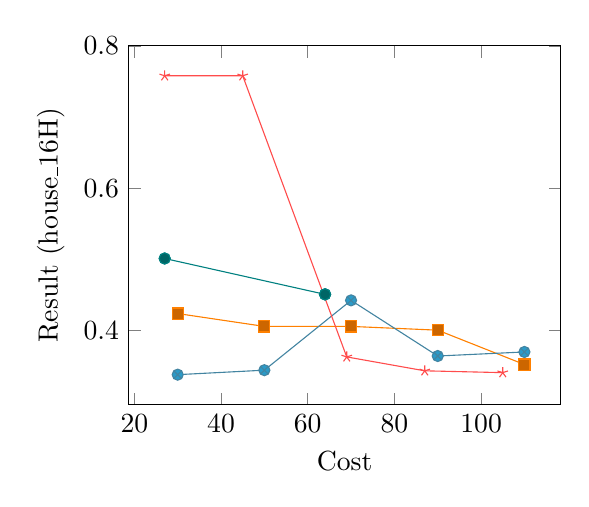
\begin{tikzpicture}
		\begin{axis}[
			xlabel = Cost,
			ylabel = Result (house\_16H),
			cycle list name=exotic,
			legend pos=outer north east,
			scale=0.8
			]
			
			\addplot coordinates
			{(27,0.5013840645551682)(27,0.5013840645551682)(64,0.4510077089071274)(64,0.4510077089071274)(64,0.4510077089071274)};
			
			\addplot coordinates 
			{(30,0.4240635335445404)(50,0.4060138463973999)(70,0.4060138463973999)(90,0.40074291825294495)(110,0.3524976521730423)};
			
			\addplot coordinates
			{(30,0.33826425671577454)(50,0.3445577770471573)(70,0.44258445501327515)(90,0.36445462703704834)(110,0.3701321929693222)};
			
			\addplot coordinates 
			{(27,0.7578987777233124)(45,0.7578987777233124)(69,0.36318539083004)(87,0.3436579704284668)(105,0.3411036729812622)};
		
			
		\end{axis}
	\end{tikzpicture}
	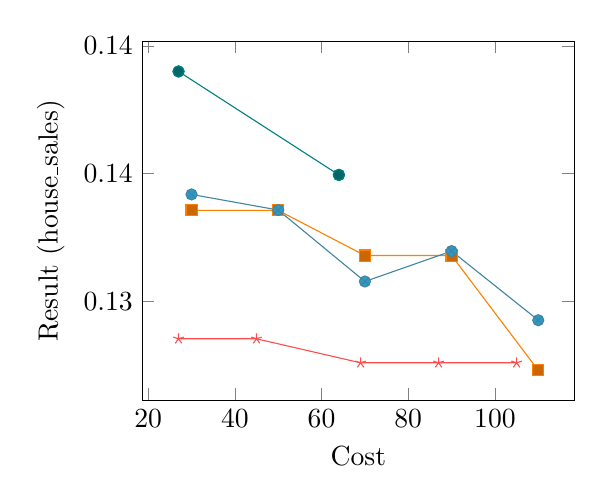
\begin{tikzpicture}
		\begin{axis}[
			xlabel = Cost,
			ylabel = Result (house\_sales),
			cycle list name=exotic,
			legend pos=outer north east,
			scale=0.8
			]
			
			\addplot coordinates
			{(27,0.1389964520931244)(27,0.1389964520931244)(64,0.1349487155675888)(64,0.1349487155675888)(64,0.1349487155675888)};
			
			\addplot coordinates 
			{(30,0.13356372714042664)(50,0.13356372714042664)(70,0.1317945420742035)(90,0.1317945420742035)(110,0.12730281800031662)};
			
			\addplot coordinates
			{(30,0.13418538868427277)(50,0.13357464969158173)(70,0.1307784542441368)(90,0.13196838647127151)(110,0.1292630285024643)};
			
			\addplot coordinates 
			{(27,0.1285368874669075)(45,0.1285368874669075)(69,0.12759799510240555)(87,0.12759799510240555)(105,0.12759799510240555)};
			
			
		\end{axis}
	\end{tikzpicture}
	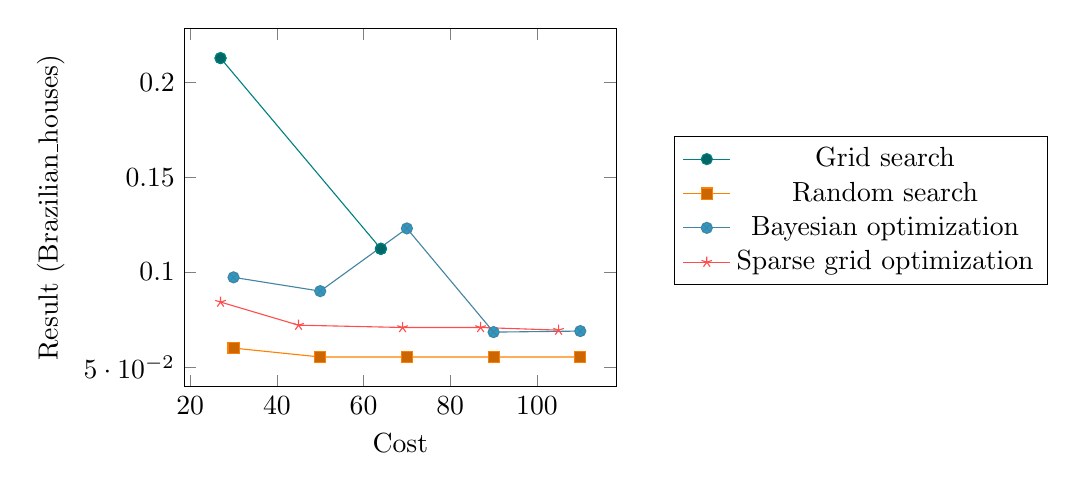
\begin{tikzpicture}
	\begin{axis}[
		xlabel = Cost,
		ylabel = Result (Brazilian\_houses),
		cycle list name=exotic,
		legend style={at={(2,0.7)}},
		scale=0.8
		]
		
		\addplot coordinates
		{(27,0.21274123340845108)(27,0.21274123340845108)(64,0.11224503070116043)(64,0.11224503070116043)(64,0.11224503070116043)};
		
		\addplot coordinates 
		{(30,0.0599429477006197)(50,0.055251454934477806)(70,0.055251454934477806)(90,0.055251454934477806)(110,0.055251454934477806)};
		
		\addplot coordinates
		{(30,0.09721800312399864)(50,0.08995457738637924)(70,0.12300247699022293)(90,0.06836232542991638)(110,0.068906981498003)};
		
		\addplot coordinates 
		{(27,0.08419231697916985)(45,0.07201046124100685)(69,0.07080245390534401)(87,0.07080245390534401)(105,0.06940628960728645)};
		
		\legend{Grid search, Random search, Bayesian optimization, Sparse grid optimization}
		
	\end{axis}
	\end{tikzpicture}
	\caption{ Comparison of grid search, random search, bayesian optimization and sparse grid search. The model optimized consists of two layers with 40 neurons each. The number of epochs, batch size, and learning rate are optimized.  }	
	\label{fig:result_second_comparison_dim3}
\end{figure}


The advantage of adaptive sparse grid optimization compared to a homogeneous grid is adaptivity meaning that more evaluations are done in a region of already small values. Especially with the house\_sales dataset, the sparse grid optimization achieves good results already with a small cost. Although in general, this method needs at least some cost to generate a grid that is precise enough to find the optimal point. This can be seen in the case of the house\_16H dataset. At first, the resulting mean average percentage error is very high compared to the other three techniques but after a cost of 69, the sparse grid optimization achieves the best results with the smallest error. \newline 

To also analyze the behavior in settings of higher dimensionality, we now also add the number of layers and the number of neurons per layer as the fourth and fifth variables to the hyperparameter space. The other variables and their intervals stay the same. The number of layers can now range from 2 to 21 and each layer can have 1 to 20 neurons. The resulting errors depending on the cost for the same three datasets as in Figure \ref{fig:result_second_comparison_dim3} can be seen in Figure \ref{fig:result_second_comparison_dim5}.


\begin{figure}[H]
	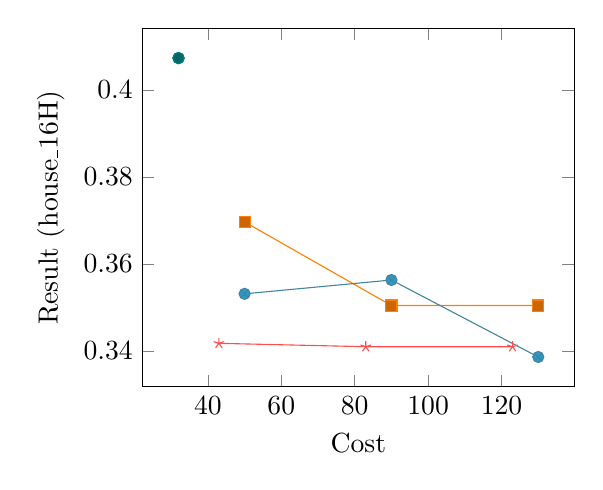
\begin{tikzpicture}
		\begin{axis}[
			xlabel = Cost,
			ylabel = Result (house\_16H),
			cycle list name=exotic,
			legend pos=outer north east,
			scale=0.8
			]
			
			\addplot coordinates
			{(32,0.40729059278964996)(32,0.40729059278964996)(32,0.40729059278964996)};
			
			\addplot coordinates 
			{(50,0.36966221034526825)(90,0.3504626899957657)(130,0.3504626899957657)};
			
			\addplot coordinates
			{(50,0.35314927995204926)(90,0.3563224822282791)(130,0.3386409282684326)};
			
			\addplot coordinates 
			{(43,0.3417779803276062)(83,0.3410039693117142)(123,0.3410039693117142)};
			
			
		\end{axis}
	\end{tikzpicture}
	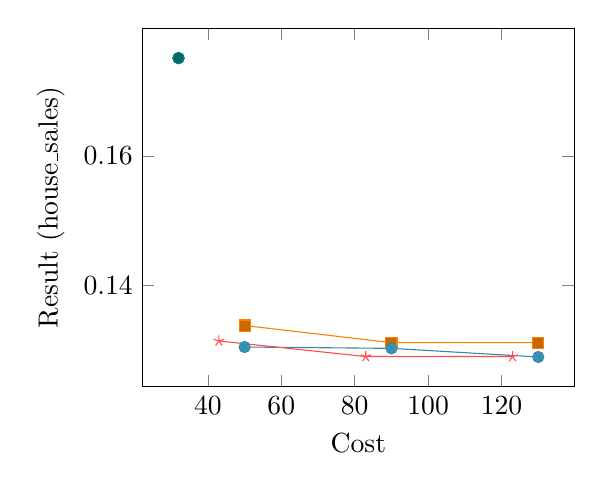
\begin{tikzpicture}
		\begin{axis}[
			xlabel = Cost,
			ylabel = Result (house\_sales),
			cycle list name=exotic,
			legend pos=outer north east,
			scale=0.8
			]
			
			\addplot coordinates
			{(32,0.1750636175274849)(32,0.1750636175274849)(32,0.1750636175274849)};
			
			\addplot coordinates 
			{(50,0.13386639952659607)(90,0.13123302906751633)(130,0.13123302906751633)};
			
			\addplot coordinates
			{(50,0.1305573582649231)(90,0.13035045564174652)(130,0.12902139127254486)};
			
			\addplot coordinates 
			{(43,0.1314886212348938)(83,0.12908799946308136)(123,0.12908799946308136)};
			
			
		\end{axis}
	\end{tikzpicture}
	\centering
	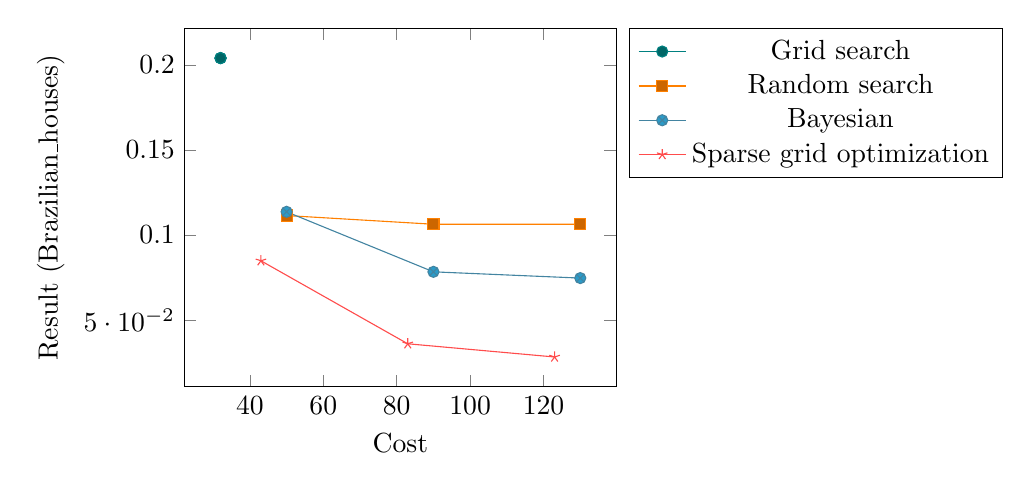
\begin{tikzpicture}
		\begin{axis}[
			xlabel = Cost,
			ylabel = Result (Brazilian\_houses),
			cycle list name=exotic,
			legend pos=outer north east,
			scale=0.8
			]
			
			\addplot coordinates
			{(32,0.20395687967538834)(32,0.20395687967538834)(32,0.20395687967538834)};
			
			\addplot coordinates 
			{(50,0.11145678907632828)(90,0.10634149610996246)(130,0.10634149610996246)};
			
			\addplot coordinates
			{(50,0.1136467456817627)(90,0.07838094979524612)(130,0.07470651902258396)};
			
			\addplot coordinates 
			{(43,0.08488190919160843)(83,0.03610859997570515)(123,0.028350481763482094)};
			
			\legend{Grid search, Random search, Bayesian, Sparse grid optimization}
			
		\end{axis}
	\end{tikzpicture}
	\caption{  Comparison of grid search, random search, bayesian optimization and sparse grid search. The number of epochs, batch size, and learning rate are optimized as well as the number of layers and number of neurons per layer. }	
	\label{fig:result_second_comparison_dim5}
\end{figure}


The big advantage of the sparse grid is the efficiency in higher dimensions. This can be seen in Figure \ref{fig:result_second_comparison_dim5}. Here with 5 dimensions and a maximum limit for a cost of 130, the normal grid search can only use 2 different values for each hyperparameter leading to 32 function evaluations. That is the reason why we can only see one point in each of the three plots for the datasets. The big advantage of sparse grid optimization is that fewer grid points are needed and those basis points generated are also adaptive to the problem leading to a fast decrease of error. For almost all three datasets, the sparse grid optimization finds the configuration leading to the smallest mean absolute percentage error. 


\subsection{Nine-dimensional Experiment with MNIST Dataset}

To also compare the different approaches with a convolutional neural network for object detection, we use a small model with the MNIST dataset. Nine different hyperparameters are optimized. An overview of the type and the ranges can be seen in Table \ref{tab:hyperparameter_space_mnist}.

\begin{table}[H]
	\caption{ Hyperparameters with their type and interval for the nine dimensional space. The values for the Int-Interval are discretized with Python's \textit{int()} function. The learning rate is sampled logarithmic and the dropout probability can take continuous values between 0 and 1. }
	\label{tab:hyperparameter_space_mnist}
	\centering
	\begin{tabular}{| c c c |} 
		\hline
		Hyperparameter & Type & Interval \\ 
		\hline
	 	Epochs & Int-Interval & $ [1,10] $ \\ 
	 	Batch size & Int-Interval & $ [200,1000] $ \\ 
	 	Learning rate & Log-Interval & $ [10^{-10},10^{-1}] $ \\ 
	 	Number conv layers & Int-Interval & $ [1,3] $ \\ 
	 	Number fully connected layers & Int-Interval & $ [1,3] $ \\ 
	 	Kernel size & Int-Interval & $ [1,4] $ \\ 
	 	Pool size & Int-Interval & $ [1,3] $ \\ 
	 	Neurons in fully connected & Int-Interval & $ [1,7] $ \\ 
	 	Dropout probability & Interval & $ [0,0.999] $ \\ 
		\hline
	\end{tabular}
\end{table}

The input shape is always $ (28, 28, 1) $ which defines the first layer of the network. After that, blocks consisting of convolutional and pooling layers are added. The number of blocks is defined by the hyperparameter number of convolutional layers. The kernel and pool size of the 2D convolution and the following pooling layer is defined by the kernel size and pool size and they are optimized. After that, fully connected layers are added. The number of layers as well as the number of neurons per layer are optimized with the two hyperparameters. Between the convolutional part and the fully connected layers, a dropout layer is added. The probability is optimized as well. The other hyperparameters like epochs, batch size, and learning rate are optimized like in the previous experiments. As an optimizer, we used the Adam optimizer and the loss function is the categorical cross-entropy. \newline 

The evaluation of the network is done as follows. The dataset is fetched with the predefined training and test set from keras. The model is fit on the training set with a validation split of $ 10\% $. It is not shuffled as we want to have reproducibility because the same hyperparameter configuration should produce the same result. This is also the reason why we reset the seeds of Python's random functions to always have the same weight initialization of the network. After the training step, we evaluate the model using the test set. As an optimization metric, we use the negative accuracy of the prediction as we still minimize. The resulting accuracy depending on the increasing cost is depicted in Figure \ref{fig:MNIST_results}.



\begin{figure}[H]
	\centering
	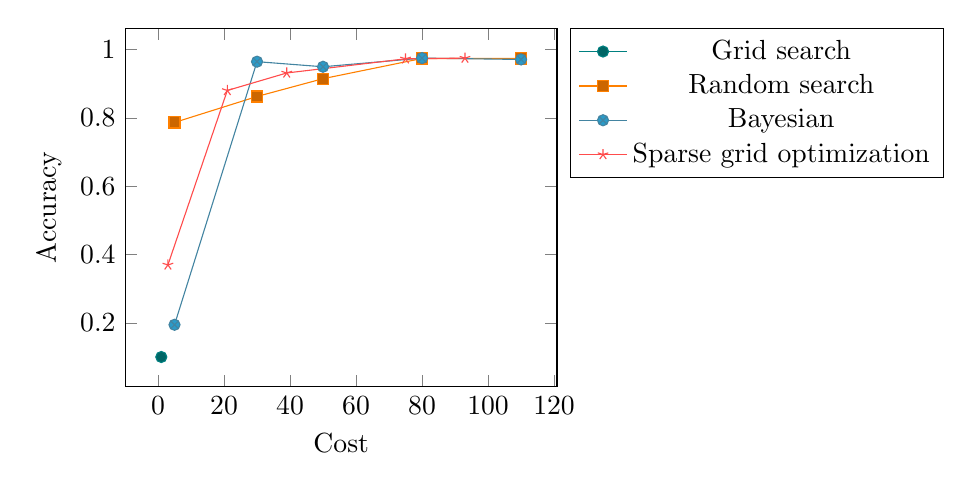
\begin{tikzpicture}
		\begin{axis}[
			xlabel = Cost,
			ylabel = Accuracy,
			cycle list name=exotic,
			legend pos=outer north east,
			scale=0.8
			]
			
			\addplot coordinates
			{(1,0.1006999984383583)};
			
			\addplot coordinates 
			{(5,0.7871000170707703)(30,0.863099992275238)(50,0.9151999950408936)(80,0.974399983882904)(110,0.974399983882904)};
			
			\addplot coordinates
			{(5,0.19499999284744263)(30,0.9649999737739563)(50,0.9501000046730042)(80,0.9753999710083008)(110,0.9714999794960022)};
			
			\addplot coordinates 
			{(3,0.3700999915599823)(21,0.8806999921798706)(39,0.9319000244140625)(75,0.9732999801635742)(93,0.9753999710083008)};
			
			\legend{Grid search, Random search, Bayesian, Sparse grid optimization}
			
		\end{axis}
	\end{tikzpicture}
	\caption{ Hyperparameter optimization of a convolutional neural network on the MNIST dataset with different algorithms. The hyperparameter intervals are presented in Table \ref{tab:hyperparameter_space_mnist}. }	
	\label{fig:MNIST_results}
\end{figure}

Again, with increasing cost, the algorithms find better configurations leading to higher accuracy. In this example, the grid search can only evaluate the model with one single configuration. This is due to the reason that the next step would be $ 2^9 = 512 $ different configurations where it would try out 2 different values for each hyperparameter. \newline 

The first points for sparse grid optimization and bayesian search are also very low, but with a bit higher cost, the performance increases very much. For the random search, even the first point with a budget of 5, the best accuracy is already at about $ 79\% $. \newline 

For the sparse grid search, the advantage compared to the normal grid search is that there is no \textit{curse of the dimensionality}. The performance is comparable with the other two algorithms, random search and bayesian optimization. \newline 

The best configurations found by each algorithm for the problem are depicted in Table \ref{tab:best_configurations_MNIST}.

\begin{table}[H]
	\caption{ Overview over the best configurations found by the different algorithms grid search (GS), random search (RS), bayesian optimization (BO) and sparse grid optimization (SG). The configuration is given as tuple (epochs, batch size, learning rate, number conv layers, number fully connected layers, kernel size, pool size, neurons per fc layer, dropout probability). }
	\label{tab:best_configurations_MNIST}
	\centering
	\begin{tabular}{| c c c c |} 
		\hline
		Algorithm & Configuration & Accuracy & Cost \\ 
		\hline
		GS & $ (5, 600, 10^{-6}, 2, 2, 2, 2, 4, 0.5) $ & $ 10.1\% $ & 1 \\ 
		RS & $ (9, 975, 0.0173, 2, 1, 3, 1, 6, 0.619) $ & $ 97.4\% $ & 80 \\ 
		BO & $ (6, 584, 10^{-2.17}, 2, 1, 3, 1, 5, 0.281) $ & $ 97.5\% $ & 80 \\ 
		SG & $ (7, 400, 10^{-2}, 2, 2, 2, 2, 5, 0.5) $ & $ 97.5\% $ & 93 \\ 
		\hline
	\end{tabular}
\end{table}

We can observe that the algorithms find different best configurations for the convolutional model. However, the resulting best accuracy is very similar. This is normal for many machine learning problems. There are many different possibilities for very good model performances. In this case, we already achieve a high accuracy of about $ 97\% $. However, it is still possible to further increase this performance by e.g. increasing the number of epochs or using a more complex neural network. But this is not what we want to analyze in this thesis. 

\subsection{Comparison with Implementation of other Authors}

A similar experiment with the same dataset is presented in \cite{WU201926}. The authors concentrate on bayesian optimization and optimize two hyperparameters. The first one is the batch size with an interval $ [20, 2000] $. The second one is the learning rate which can take values from $ [0,1] $. The network that is used for predicting the class of the images is a small convolutional neural network. The architecture can be seen in Table \ref{tab:architecture_MNIST_comp}.


\begin{table}[H]
	\caption{ Architecture used in \cite{WU201926} for MNIST image classification. }
	\label{tab:architecture_MNIST_comp}
	\centering
	\begin{tabular}{| c c c c |} 
		\hline
		Type & Filters  & Kernel size & Activation function \\ 
		\hline
		Convolutional 2D & 32 & $ (5,5) $ & ReLU \\ 
		Max Pooling 2D &  & $ (2,2) $ &  \\ 
		Convolutional 2D & 32 & $ (5,5) $ & ReLU \\ 
		Max Pooling 2D &  & $ (2,2) $ &  \\ 
		Dense &  &  & Softmax \\ 
		\hline
	\end{tabular}
\end{table}

As an optimizer, they used the gradient descent and the loss function is the categorical cross-entropy. The metric to be optimized is accuracy. \newline 

In \cite{WU201926}, it is not described for how many epochs they train the neural network which makes it hard to directly compare the algorithms. Additionally, we set the interval of the batch size to $ [20, 1020] $ because of hardware limitations. The learning rate is in our case again a logarithmic hyperparameter with a lower bound of $ 10^{-16} $ and an upper bound of $ 1 $. For the neural network evaluation, we train the model on the training set with a validation split of $ 10\% $. The resulting score is then defined as the accuracy of the predictions of the test set. The result of the experiment with our four different algorithms is presented in Figure \ref{fig:Comparison_MNIST}.


\begin{figure}[H]
	\centering
	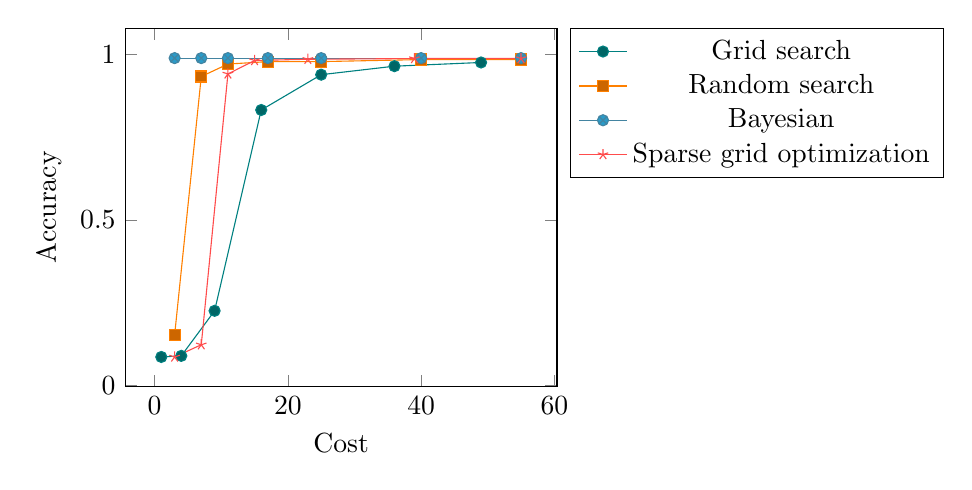
\begin{tikzpicture}
		\begin{axis}[
			xlabel = Cost,
			ylabel = Accuracy,
			cycle list name=exotic,
			legend pos=outer north east,
			scale=0.8
			]
			
			\addplot coordinates
			{(1,0.0860000029206276)(4,0.0892999991774559)(9,0.22550000250339508)(16,0.8327000141143799)(25,0.9394999742507935)(36,0.9652000069618225)(49,0.9764000177383423)};
			
			\addplot coordinates 
			{(3,0.15240000188350677)(7,0.9340000152587891)(11,0.9715999960899353)(17,0.9789999723434448)(25,0.9789999723434448)(40,0.9851999878883362)(55,0.9851999878883362)};
			
			\addplot coordinates
			{(3,0.9896000027656555)(7,0.9896000027656555)(11,0.9896000027656555)(17,0.9896000027656555)(25,0.9896000027656555)(40,0.9896000027656555)(55,0.9896000027656555)};
			
			\addplot coordinates 
			{(3,0.0860000029206276)(7,0.12290000170469284)(11,0.9416999816894531)(15,0.9824000000953674)(23,0.9861000180244446)(39,0.9883000254631042)(55,0.9883000254631042)};
			
			\legend{Grid search, Random search, Bayesian, Sparse grid optimization}
			
		\end{axis}
	\end{tikzpicture}
	\caption{ Resulting accuracy with increasing budget for the grid search, random search, bayesian optimization and sparse grid optimization. The MNIST dataset and a small convolutional neural network were used. }	
	\label{fig:Comparison_MNIST}
\end{figure}

Again, with increasing cost, the performance of the optimization techniques improves. The absolute highest accuracy is achieved by the bayesian optimization with $ 98.96\% $ followed by the sparse grid optimization with $ 98.83\% $, and random search with $ 98.52\% $. The lowest accuracy is achieved by grid search with a value of $ 97.64\% $. The authors of \cite{WU201926} reach an accuracy of $ 99.14\% $ with a budget of 50, however, we do not know for how many epochs they trained the network. For the evaluation of our four algorithms, we always used exactly ten epochs. The best configurations found by the techniques are depicted in Table \ref{tab:configs_MNIST_comp}. \newline 

\begin{table}[H]
	\caption{ Best configurations and corresponding test accuracy found by the four algorithms for the MNIST dataset. }
	\label{tab:configs_MNIST_comp}
	\centering
	\begin{tabular}{| c c c c |} 
		\hline
		Algorithm & Batch size & Learning rate & Accuracy \\ 
		\hline
		Grid search & 91 & 0.01000 & 0.9764 \\ 
		Random search & 42 & 0.03448 & 0.9852 \\ 
		Bayesian optimization & 57 & 0.1979 & 0.9896 \\ 
		Sparse grid optimization & 270 & 0.3162 & 0.9883 \\ 
		\hline
	\end{tabular}
\end{table}

The results shown in Table \ref{tab:configs_MNIST_comp} indicate that in this case, a rather small batch size leads to better testing results. This shows that the reduced interval is not restricting the performance of our algorithms. For this experiment, the authors in \cite{WU201926} do not provide the configuration found by their algorithm which makes it hard to compare the performances. 


\section{Iterative Adaptive Random Search}

In the previous analysis of the sparse grid optimization for finding suitable hyperparameter configurations, we have seen that using sparse grids has advantages compared to the other algorithms in some situations. However, pure random search is very powerful in most cases. One possible adaption of this method is to add iterative refinement like it is done in the grid generation of sparse grids. This is a promising way of combining the advantages of iterative methods and random search which allows to evaluate many different values for each hyperparameter. This is why we introduce a new algorithm for optimizing the hyperparameters of machine learning models in an efficient manner.

\subsection{Implementation}

The algorithm starts with initial points that are distributed randomly in the whole search space. The number of these first points is variable and can be given by the user. A suitable value is dependent on the problem and the number of hyperparameters to be optimized. In each following iteration, one point is selected to be refined. The refinement criterion is similar to the Ritter-Novak criterion used for the sparse grid generation. The point i that minimizes 
\begin{equation}
\label{eq:refinement_criterion}
	(rank_i + 1)^{1-\gamma} \cdot (level_i + refinements_i + 1)^\gamma
\end{equation} 
is refined. Here, the rank is the position of the point in the list of all points with ascending function values. The adaptivity parameter $ \gamma $ can be used to balance exploration and exploitation. Each point additionally has an attribute level which is 0 for the initial points. In each iteration, the level of the added points is one higher than the level of the refined point. The refinements attribute is increased each time the point is refined. \newline

For the refinement strategy, meaning where the points are added, random points are sampled following a distribution on a specific domain. There are different possible techniques for refinement. In general, the algorithm takes the steps as depicted in Algorithm \ref{alg:adaptive_random_search_alg}. The iterations take place as long as the number of points where the function is evaluated is smaller or equal to the budget which has to be given.

\begin{algorithm}[H]
	\caption{ Iterative adaptive random search for hyperparameter optimization. In each iteration, a random point is sampled following a specific distribution depending on the refinement criterion. }
	\label{alg:adaptive_random_search_alg}
	\textbf{Input} \textbf{m}: number of initial points, \textbf{n}: number of refinements per iteration, \textbf{budget}: upper bound for evaluations, \boldmath{ $ \gamma $}: adaptivity parameter\\
	\textbf{Output} \textbf{points}: Array of all evaluated points
	\begin{algorithmic}
		\For{\texttt{min(m, budget)}}
			\State \texttt{sample point uniformly in search space}
			\State \texttt{add point with level 0 to array}
		\EndFor
		\While{Number of points + n <= budget}
			\State \texttt{sort points with ascending function value}
			\State \texttt{select point p\_ref according to refinement criterion}
			\For{\texttt{n}}
				\State \texttt{sample point according to refinement strategy}
				\State \texttt{add point with level p\_ref.level + 1}
				\State \texttt{increase p\_ref.refinements}
			\EndFor
			\State \texttt{increase number of points by n}
		\EndWhile
		\State return array of points
	\end{algorithmic}
\end{algorithm}

As input, the algorithm \ref{alg:adaptive_random_search_alg} expects the number of initial points m, the number of points to be added in each iteration, the upper bound for the number of function evaluations called budget and the adaptivity parameter $ \gamma $. The overall output is the array of all points where the function was evaluated. 

The first loop is for sampling the initial points. The number of iterations is defined with \texttt{min(m, budget)} to assure that the number of function evaluations is smaller or equal to the budget. All initial points have level 0. 

In the following, the refinements are done in the loop as long as the budget is not exceeded. First, the array is sorted with the ascending function value. Then, one point is selected based on the refinement criterion \ref{eq:refinement_criterion}. The rank of the point is then just the index in the sorted array. 

In the next loop which is iterated n times, a new point is sampled according to the concrete refinement strategy. This point is then added with a level which is one higher than the one selected to be refined. Additionally, the \texttt{refinements} parameter of the point selected is increased by one. \newline 

The general idea of the refinement strategy is to sample points which are near to the point that is being refined because this point is either promising due to a small function value and thus rank, or it has not been refined that often. Concretely, we provide three different strategies which are presented in the following.

\subsubsection{Interval Based Refinement Strategy}

For this first refinement strategy, intervals in each dimension are used. The bounds are defined by neighboring points with and the sampling is done uniformly. An example for such a refinement is presented in Figure \ref{fig:alternative_1}. \newline 

\begin{figure}[H]
	\centering
	\includegraphics[scale=0.8]{figures/Adaptive_random/Visualizations/Alternative_1}
	\caption{ Example for the interval based refinement strategy. The point being refined is indicated with the blue cross and the lines show the upper and lower boundary in each direction. The sampling is done uniformly in the blue area. }
	\label{fig:alternative_1}
\end{figure}

In the example in Figure \ref{fig:alternative_1}, the number of initial points is 5. The point with the blue cross is selected by the refinement criterion defined with \ref{eq:refinement_criterion}. In each dimension, an interval is defined with the bounds from the next points in each dimension. In this case, the interval in the horizontal direction is $ [-4.151, 5.045] $ and in the vertical dimension $ [-0.3779, 6.039] $. Note that only points with the same or smaller level are considered when building the interval.

\subsubsection{Uniform D-Ball Sampling Strategy}

This strategy is based on uniform sampling inside a multi-dimensional ball. The point that is refined is the center of this ball and we define a certain radius of the ball. For the uniform sampling, multiple possible algorithms exist \cite{HARMAN20102297}. Some of them suffer from the curse of the dimensionality. One example is the rejection method where a value from $ [0,1]^d $ is sampled and rejected if it is not inside the ball. The probability of a sample being rejected increases with higher dimensionality. Another method is using the normal distribution. For a random variable $ Y \sim N_d(0_d, 1_d) $, $ S_n = \frac{Y}{|| Y ||} $ is uniformly distributed on the d-sphere which is the surface of the ball. The last step is to multiply $ S_n $ by $ U^{\frac{1}{d}} $ where $ U $ has the uniform distribution on the interval between 0 and 1. Now the sampling is done inside the standard d-ball with a radius of 1. The final value just has to be multiplied by the radius to change the sampling to a d-ball with an arbitrary size. One two-dimensional example can is presented in Figure \ref{fig:alternative_2}.

\begin{figure}[H]
	\centering
	\includegraphics[scale=0.8]{figures/Adaptive_random/Visualizations/Alternative_2}
	\caption{ Example for the uniform d-ball sampling strategy. The point being refined is indicated with the blue cross and the circle is the area where the uniform sampling is done. }
	\label{fig:alternative_2}
\end{figure}

In the example depicted in Figure \ref{fig:alternative_2}, five initial points (colored in red) are sampled. The one marked with the blue cross is chosen to be refined in this iteration. The radius is depending on the level of the point and the smallest and maximum distance to other points. It is computed with
\begin{equation}
	r = \frac{dist_{max} + dist_{min}}{(level+2)\cdot 2}
\end{equation}

where $ dist_{max} $ and $ dist_{min} $ are the highest and lowest distance to other points, respectively. The $ level $ is the level of the current point that is refined. With this, the radius of the ball at points with higher levels is smaller leading to samples near to the point being refined.

\subsubsection{Normal Distribution Sampling Strategy}

The last alternative is not sampling uniformly but based on the normal distribution. The idea behind this strategy is that we might be interested in sampling new points near the one that has to be refined in this iteration. This might lead to better results because the point that is refined might already be very promising. Therefore, in each dimension, the coordinate is sampled. A two-dimensional example is presented in Figure \ref{fig:alternative_3}.

\begin{figure}[H]
	\centering
	\includegraphics[scale=0.8]{figures/Adaptive_random/Visualizations/Alternative_3}
	\caption{ Example for the normal distribution sampling strategy. The point being refined is indicated with the blue cross and contour represents the likelihood of samples. }
	\label{fig:alternative_3}
\end{figure}

The example in Figure \ref{fig:alternative_3} shows five initial points in red. The point marked with the blue cross is refined in this iteration step. The contour plot in the background indicates the probability distribution for new points. In each dimension, a normal distribution is constructed with mean and standard deviation with 
\begin{equation}
	\begin{split}
		dist =& \frac{dist_{max} + dist_{min}}{(level+2)\cdot 2} \\
		lower =& \text{ min}(\text{ max}(coord - dist, bound_{lower}), bound_{upper}) \\
		upper =& \text{ max}(\text{ min}(coord + dist, bound_{upper}), bound_{lower}).
	\end{split}
\end{equation}

Here, $ coord $ is the coordinate of the point refined in the corresponding dimension, $ bound_{lower} $ and $ bound_{upper} $ represent the bounds of the interval of the hyperparameter in this dimension and the distance $ dist $ is calculated the same way as the radius of the second refinement strategy. Additionally, after sampling a point, it is ensured that the point lays inside the search space with 

\begin{equation}
	\begin{split}
		coordinate =& \text{ max}((coordinate, bound_{lower})) \\
		coordinate =& \text{ min}((coordinate, bound_{upper})).
	\end{split}
\end{equation}

This is done for each dimension so that for all $ coordinate $ variables drawn, the sample is not higher than the upper bound and not lower than the lower bound in each dimension. \newline 

For the implementation, we added a new subclass inheriting \texttt{Optimization}. It has an additional parameter for the choice of refinement strategy. 

\subsection{Analysis of Parameters with Functions}

In this case, we also have the problem that the optimal configuration of hyperparameters for the model evaluation is not known in advance. This is why we first analyze the algorithm with functions where we know the optimum. We will especially focus on the following parameters of the adaptive random search:

\begin{itemize}
	\item Adaptivity parameter
	\item Number of initial points
	\item Number of refinements per iteration
	\item Refinement criterion
	\item Budget
\end{itemize}

We will optimize the Rosenbrock function (see Table \ref{tab:test_functions} and Figure \ref{fig:test_functions_plot}) in two dimensions for additional visualization. The optimal point is at $ (1, 1) $ with a function value of 0. 

\subsubsection{Adaptivity Parameter}

The first parameter we want to analyze is the adaptivity parameter $ \gamma $ to check if the algorithm behaves as expected. Especially the refinement criterion and strategy are influencing the behavior depending on this parameter. Therefore, we want to visualize how the points are distributed depending on the concrete value. We optimize the Rosenbrock function (see Table \ref{tab:test_functions} and Figure \ref{fig:test_functions_plot}) in two dimensions to visualize the resulting points. The optimal point is at $ (1, 1) $ with a function value of 0. The results with a 200 budget and 5 initial points are depicted in Figure \ref{fig:Adapt_param_alternatives}.


\begin{figure}[H]
	\begin{subfigure}{\textwidth}
		\centering
		\includegraphics[width=0.31\textwidth]{figures/Adaptive_random/Adaptivity_parameter/Alternative_0_adapt_1.0}
		\includegraphics[width=0.31\textwidth]{figures/Adaptive_random/Adaptivity_parameter/Alternative_0_adapt_0.75}
		\includegraphics[width=0.31\textwidth]{figures/Adaptive_random/Adaptivity_parameter/Alternative_0_adapt_0.0}
		\caption{ Resulting points for the \textbf{interval based refinement strategy}. Adaptivity parameter $ \gamma $: 1.0 (left), 0.75 (center), 0.0 (right). }
		\label{fig:alt0_adapt_param}
	\end{subfigure}
	\begin{subfigure}{\textwidth}
		\centering
		\includegraphics[width=0.31\textwidth]{figures/Adaptive_random/Adaptivity_parameter/Alternative_1_adapt_1.0_1_}
		\includegraphics[width=0.31\textwidth]{figures/Adaptive_random/Adaptivity_parameter/Alternative_1_adapt_0.75}
		\includegraphics[width=0.31\textwidth]{figures/Adaptive_random/Adaptivity_parameter/Alternative_1_adapt_0.0_1_}
		\caption{ Resulting points for the \textbf{uniform d-ball sampling strategy}. Adaptivity parameter $ \gamma $: 1.0 (left), 0.75 (center), 0.0 (right). }
		\label{fig:alt1_adapt_param}
	\end{subfigure}
	\begin{subfigure}{\textwidth}
		\centering
		\includegraphics[width=0.31\textwidth]{figures/Adaptive_random/Adaptivity_parameter/Alternative_2_adapt_1.0_2_}
		\includegraphics[width=0.31\textwidth]{figures/Adaptive_random/Adaptivity_parameter/Alternative_2_adapt_0.75}
		\includegraphics[width=0.31\textwidth]{figures/Adaptive_random/Adaptivity_parameter/Alternative_2_adapt_0.0_2_}
		\caption{ Resulting points for the \textbf{normal distribution sampling strategy}. Adaptivity parameter $ \gamma $: 1.0 (left), 0.75 (center), 0.0 (right). }
		\label{fig:alt2_adapt_param}
	\end{subfigure}
	
	\caption{ Generated points for optimizing the Rosenbrock function with interval based refinement strategy (\ref{fig:alt0_adapt_param}), uniform d-ball sampling strategy (\ref{fig:alt1_adapt_param}), and normal distribution sampling strategy (\ref{fig:alt2_adapt_param}). In each case, the left one has adaptivity parameter $ \gamma = 1.0 $ which distributes the points most homogeneous. In the center with $ \gamma = 0.75 $, they are concentrated on few areas and in each right case where $ \gamma = 0.0 $, the grid is most adaptive and almost all points are in the same region. }
	\label{fig:Adapt_param_alternatives}
\end{figure}

The resulting points in Figure \ref{fig:Adapt_param_alternatives} show the behavior of the algorithms depending on the adaptivity parameter $ \gamma $. In all three cases, the points are most distributed in the whole domain for $ \gamma = 1.0 $ (left grids). This is due to the refinement criterion \ref{eq:refinement_criterion} which then selects the candidates in that way, that all points are refined as equally as possible which makes the distribution very homogeneous. In the center cases with $ \gamma = 0.75 $, the trade-off between selecting points that have low rank and ones that have not been refined that often is balanced. The second extreme case is with $ \gamma = 0.0 $. This always leads to the candidate point with the smallest rank (smallest function value). This can be seen in the grid because the points are not distributed at all. Note that you can directly see the difference between the uniform d-ball sampling strategy (\ref{fig:alt1_adapt_param}, right grid) and the normal distribution sampling strategy (\ref{fig:alt2_adapt_param}, right grid) because in the first case, the points are distributed uniformly in this circle and in the lower strategy, the density of points is higher in the center of the region around $ (1,1) $. \newline 

The concrete optimum found in each case is presented in Table \ref{tab:results_alternatives}.

\begin{table}[H]
	\caption{ Resulting optimum found by the three different refinement strategies interval based refinement strategy (1), uniform d-ball sampling strategy (2), and normal distribution sampling strategy (3). The best of each refinement algorithm is marked in bold. }
	\label{tab:results_alternatives}
	\centering
	\begin{tabular}{| c |  c |c c |} 
		\hline
		Alternative & Adaptivity parameter & Coordinates & Error \\ 
		\hline
		%1 & 1.0 & [0.4058562472117627, -0.04054645111546973] & 4.566409386159776 \\ 
		%1 & 0.75 & [1.038927050174919, 1.079563922856002] & 0.001519098543161749 \\ 
		%1 & 0.0 & [2.158598821574482, 4.617743382926759] & 1.517121125222536 \\ 
		
		%2 & 1.0 & [-0.11352135098080107, -0.7217782890446469] & 55.21325276318493 \\ 
		%2 & 0.75 & [1.6268172463461463, 2.6253824302103714] & 0.43764024412597213 \\ 
		%2 & 0.0 & [0.9541974556509123, 0.9027712932595593]  & 0.008060015566753589 \\ 
		
		%3 & 1.0 & [2.2818252596693043, 4.712738873843234] & 26.04545502357817 \\ 
		%3 & 0.75 & [0.9605735775731732, 0.838958015201549] & 0.7028532076339621 \\ 
		%3 & 0.0 & [1.097943243714717, 1.1936061770810482] & 0.02369014149435738 \\ 
		
		 & 1.0 & [0.4059, -0.04055] & 4.566 \\ 
		1 & 0.75 & \textbf{[1.039, 1.080]} & \textbf{0.001519} \\ 
		 & 0.0 & [2.159, 4.618] & 1.517 \\ 
		\hline
		 & 1.0 & [-0.1135, -0.7218] & 55.21 \\ 
		2 & 0.75 & [1.627, 2.625] & 0.4376 \\ 
		 & 0.0 & \textbf{[0.9542, 0.9028]}  & \textbf{0.008060} \\ 
		\hline
		 & 1.0 & [1.305, 1.598] & 1.208 \\ 
		3 & 0.75 & [1.465, 2.265] & 1.651 \\ 
		 & 0.0 & \textbf{[1.098, 1.194]} & \textbf{0.02369} \\ 
		
		\hline
	\end{tabular}
\end{table}

Table \ref{tab:results_alternatives} shows that each of the algorithms finds a point very near to the optimum which is at $ (1,1) $. The table also indicates that each refinement strategy has a different best adaptivity parameter. For the second two alternatives, the most adaptive grid achieves the best result while a more homogeneous one is better for the first algorithm. \newline 

The experiments by now were only made with 3 distinct values for the adaptivity parameter and this only leads to assumptions that the evaluated parameters are the best in each case. To further analyze this parameter, the Rosenbrock and additionally, the Rastrigin function were solved with 11 different adaptivity parameters between 0 and 1 with a step size of $ 0.1 $. The results for each of the three algorithms are presented in Figure \ref{fig:alternatives_adaptivities_plot}.

\begin{figure}[H]
	\centering
	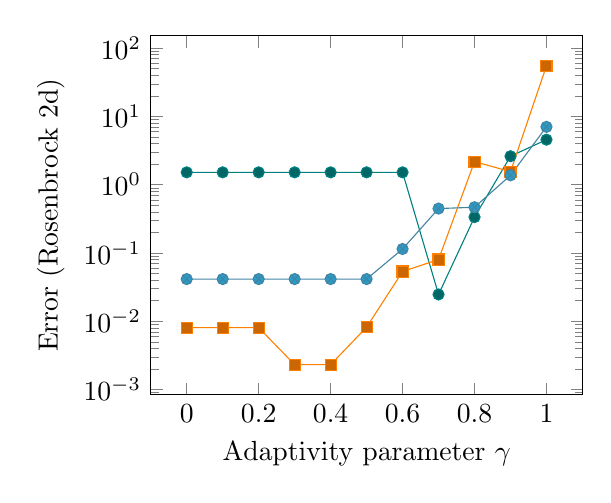
\begin{tikzpicture}
		\begin{axis}[
			xlabel = Adaptivity parameter $ \gamma $,
			ylabel = Error (Rosenbrock 2d),
			cycle list name=exotic,
			cycle list name=exotic,
			legend style={at={(1.03,0.5)},anchor=west},
			scale=0.8,
			ymode=log,
			]
			
			\addplot coordinates
			{(0.0,1.517121125222536)(0.1,1.517121125222536)(0.2,1.517121125222536)(0.30000000000000004,1.517121125222536)(0.4,1.517121125222536)(0.5,1.517121125222536)(0.6000000000000001,1.5171211252086616)(0.7000000000000001,0.02466439437702513)(0.8,0.33502340624824123)(0.9,2.61442204654008)(1.0,4.566409386159776)}
			;
			
			\addplot coordinates 
			{(0.0,0.008060015566753589)(0.1,0.008060015566753589)(0.2,0.008060015566753589)(0.30000000000000004,0.0023118954614058484)(0.4,0.002311894614521982)(0.5,0.008182947611344513)(0.6000000000000001,0.05339618203112462)(0.7000000000000001,0.08011233075458785)(0.8,2.1785202665483165)(0.9,1.5532894112998432)(1.0,55.21325276318493)}
			;
			
			\addplot coordinates
			{(0.0,0.04143540730358583)(0.1,0.04143540730358583)(0.2,0.04143540730358583)(0.30000000000000004,0.04143540730358583)(0.4,0.04143540730358583)(0.5,0.04143540730358583)(0.6000000000000001,0.1143331623160982)(0.7000000000000001,0.44676242767744595)(0.8,0.4676312056273927)(0.9,1.3722867702638328)(1.0,7.035490443472938)};
						
			
		\end{axis}
	\end{tikzpicture}
	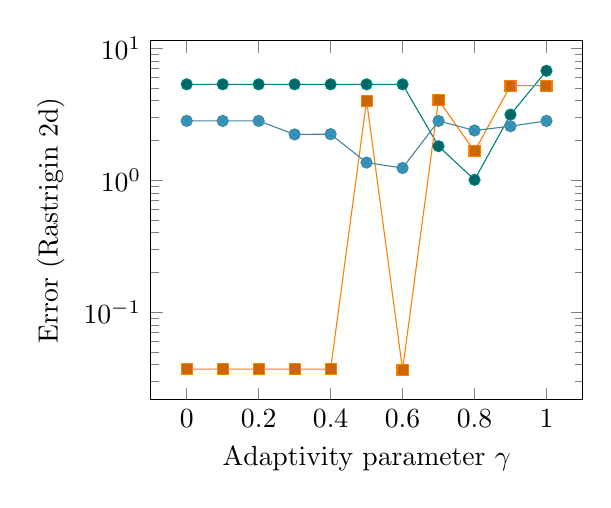
\begin{tikzpicture}
		\begin{axis}[
			xlabel = Adaptivity parameter $ \gamma $,
			ylabel = Error (Rastrigin 2d),
			cycle list name=exotic,
			legend style={at={(1.03,0.5)},anchor=west},
			scale=0.8,
			ymode=log,
			]
			
			\addplot coordinates
			{(0.0,5.321259851862457)(0.1,5.321259851862457)(0.2,5.321259851862457)(0.30000000000000004,5.321259851862457)(0.4,5.321259851862457)(0.5,5.321259851862457)(0.6000000000000001,5.321001698568752)(0.7000000000000001,1.8077635146255417)(0.8,1.0048622402760152)(0.9,3.1362207781035067)(1.0,6.738058570648082)}
			;
			
			\addplot coordinates 
			{(0.0,0.0370187636704884)(0.1,0.0370187636704884)(0.2,0.0370187636704884)(0.30000000000000004,0.0370187636704884)(0.4,0.0370187636704884)(0.5,4.003244844322138)(0.6000000000000001,0.03662386784840521)(0.7000000000000001,4.046206137247143)(0.8,1.6528238414282015)(0.9,5.200127399463108)(1.0,5.200127399463108)}
			;
			
			\addplot coordinates
			{(0.0,2.8098752567524095)(0.1,2.8098752567524095)(0.2,2.8098752567524095)(0.30000000000000004,2.2197551375481552)(0.4,2.229984769660202)(0.5,1.3588875496246118)(0.6000000000000001,1.235250528609047)(0.7000000000000001,2.8098752567524095)(0.8,2.37673379617285)(0.9,2.562928198839309)(1.0,2.8098752567524095)};
			
			
		\end{axis}
	\end{tikzpicture}
	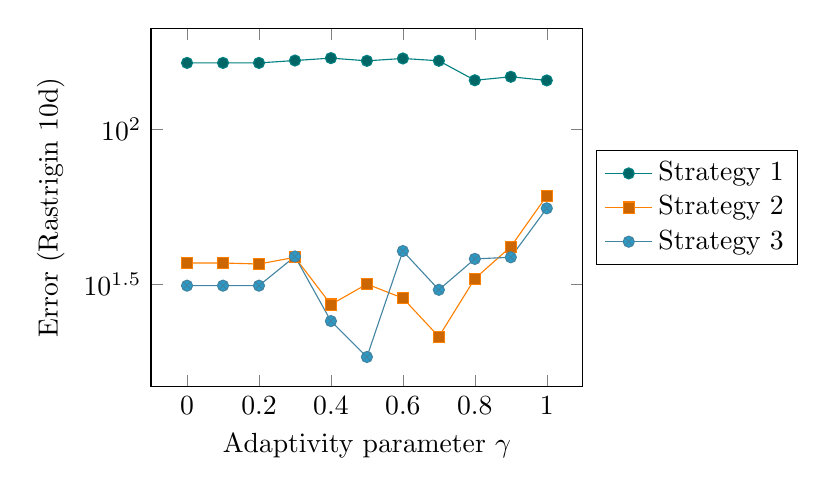
\begin{tikzpicture}
		\begin{axis}[
			xlabel = Adaptivity parameter $ \gamma $,
			ylabel = Error (Rastrigin 10d),
			cycle list name=exotic,
			legend style={at={(1.03,0.5)},anchor=west},
			scale=0.8,
			ymode=log,
			]
			
			\addplot coordinates
			{(0.0,162.761025073682)(0.1,162.761025073682)(0.2,162.761025073682)(0.30000000000000004,165.65760013033167)(0.4,168.64616716760546)(0.5,165.2768663253831)(0.6000000000000001,168.1834839451662)(0.7000000000000001,165.35086318493714)(0.8,143.1580199831282)(0.9,146.8933255133596)(1.0,142.9938345967389)}
			;
			
			\addplot coordinates 
			{(0.0,37.09356147694522)(0.1,37.09356147694522)(0.2,36.81602227605653)(0.30000000000000004,38.68156741616422)(0.4,27.282614603454675)(0.5,31.73913303273261)(0.6000000000000001,28.605152304899946)(0.7000000000000001,21.519348408206483)(0.8,33.04214109501011)(0.9,41.83500106274237)(1.0,60.94266017470839)}
			;
			
			\addplot coordinates
			{(0.0,31.371096705820833)(0.1,31.371096705820833)(0.2,31.371096705820833)(0.30000000000000004,38.922820229144364)(0.4,24.140387463402618)(0.5,18.51902820363044)(0.6000000000000001,40.51677991948232)(0.7000000000000001,30.425044718671558)(0.8,38.233466954045774)(0.9,38.69731668001502)(1.0,55.559856664944796)};
			
			\legend{Strategy 1, Strategy 2, Strategy 3}
			
			
		\end{axis}
	\end{tikzpicture}
	\caption{ Error of the found optimum by the different refinement strategies for the Rosenbrock (2d) and the Rastrigin (2d and 10d) functions. For the two-dimensional case, the budget is 200 and for the 10-d optimization the budget is set to 5000. }	
	\label{fig:alternatives_adaptivities_plot}
\end{figure}

The results in Figure \ref{fig:alternatives_adaptivities_plot} confirm that each strategy has its own "sweet spot" for the adaptivity parameter. Additionally, the best value depends on the function used as you can see in the upper row (Rosenbrock and Rastrigin 2d). For strategy 1, the best result is achieved with $ \gamma = 0.7 $ for Rosenbrock, and for Rastrigin, the best value is 0.8. Furthermore, the value not only depends on the function but also on the dimension of the input. For example for strategy 2, very good results are achieved with small values $ 0.0 \le \gamma \le 0.4 $ and $ \gamma = 0.6 $ in two dimensions. However, in the ten-dimensional case, the best value is $ \gamma = 0.7 $. This is due to the behavior of the probability distributions in higher dimensions. We can roughly follow that for higher dimension, we need lower adaptivity (higher adaptivity parameter $ \gamma $).

\subsubsection{Number of initial points}

The second parameter we want to analyze is the number of initial points. Intuitively, a high value for this parameter makes the algorithm behave more similarly to the normal random search because more random points on the whole domain are sampled and fewer refinement steps are done. We, therefore, optimize the three test functions Rosenbrock, Rastrigin, and Eggholder with a different number of initial points and compare the Errors of the optimum found. The overall budget is 200 and the results are shown in Figure \ref{fig:init_points_alternatives}. In each case, 10 runs are evaluated and the average error is plotted. For the adaptivity parameters, we set $ \gamma_1 = 0.75 $, $ \gamma_2 = 0.35 $, and $ \gamma_3 = 0.6 $ for the two-dimensional cases and the three refinement strategies, respectively. For $ d = 4 $, we have $ \gamma_1 = 0.85 $, $ \gamma_2 = 0.45 $, and $ \gamma_3 = 0.7 $ and for $ d = 6 $, we set $ \gamma_1 = 0.9 $, $ \gamma_2 = 0.65 $, and $ \gamma_3 = 0.8 $ \newline

\begin{figure}[H]
	\centering
	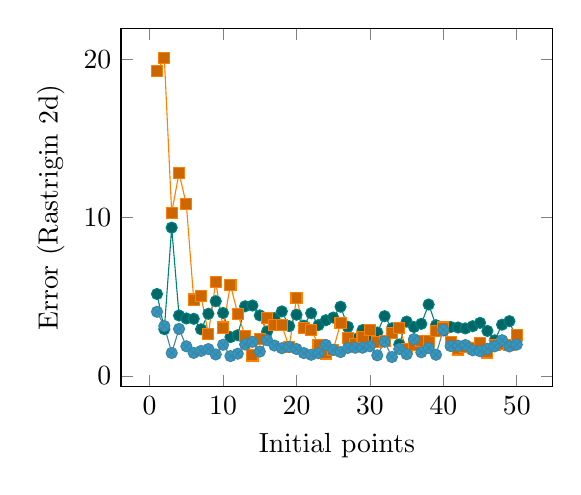
\begin{tikzpicture}
		\begin{axis}[
			xlabel = Initial points,
			ylabel = Error (Rastrigin 2d),
			cycle list name=exotic,
			legend style={at={(1.03,0.5)},anchor=west},
			scale=0.8,
			%ymode=log,
			]
			
			\addplot coordinates
			{(1,5.16541885283579)(2,2.9471829226125923)(3,9.356453291854786)(4,3.808304049785871)(5,3.61941506608414)(6,3.5969268742002676)(7,2.9376792078042517)(8,3.9143744644885112)(9,4.709905855330143)(10,3.968632255586376)(11,2.443182643124446)(12,2.561347925976516)(13,4.389034414267667)(14,4.436976838474754)(15,3.8150092540477316)(16,2.802813683144063)(17,3.641326069196926)(18,4.06665375179009)(19,3.13865289389336)(20,3.8570487168053047)(21,3.1600648317572664)(22,3.95417562025947)(23,3.2020515827225373)(24,3.5086215559300284)(25,3.67563897265263)(26,4.36238311330542)(27,3.0940382063589835)(28,2.306577070672033)(29,2.8860131740360884)(30,2.5155478898576358)(31,2.731838795029469)(32,3.7649507141935397)(33,2.998552118566761)(34,1.9786325984112239)(35,3.4201680080260366)(36,3.081055976736389)(37,3.279204147165418)(38,4.500408958754233)(39,3.192073208303711)(40,2.8634530481015164)(41,3.082409213858928)(42,3.047459671452304)(43,2.9917458852115373)(44,3.131097459097421)(45,3.3425055525016547)(46,2.832216899598248)(47,2.240591866384464)(48,3.2285467053945167)(49,3.4504921973191474)(50,2.2449499885654562)}
			;
			
			\addplot coordinates 
			{(1,19.254967736212873)(2,20.0636179559963)(3,10.296775534383103)(4,12.803152545732171)(5,10.823735892006274)(6,4.815163935635113)(7,5.015182510229806)(8,2.6492149703540333)(9,5.919781359015478)(10,3.044929330327495)(11,5.749023953682593)(12,3.907736379638817)(13,2.5310018286439666)(14,1.2830471598576476)(15,2.3467204016909684)(16,3.6744177220632652)(17,3.189351348885487)(18,3.2155704039324733)(19,1.8003432910152497)(20,4.911301945293574)(21,3.0351347068485723)(22,2.8932239242675712)(23,1.947959965629304)(24,1.4117265569966264)(25,1.6326773103637842)(26,3.3101706184654573)(27,2.362589881274289)(28,2.007331489515397)(29,2.438652634766208)(30,2.907085133714194)(31,2.1531399602396655)(32,2.2012922777695056)(33,2.6764207831282696)(34,3.0154446171828715)(35,1.6929630156256035)(36,1.9425151955291518)(37,2.1898733680430533)(38,2.187451017831427)(39,2.809755045745188)(40,3.0438867936920424)(41,2.104909792157456)(42,1.6619447559606304)(43,1.7976585495338768)(44,1.737965435705192)(45,2.0406703497513936)(46,1.4755966970797396)(47,1.9558237218991)(48,1.9907440783909363)(49,1.9603281242106683)(50,2.5625366487936425)}
			;
			
			\addplot coordinates
			{(1,4.040638936432708)(2,3.1417233610631596)(3,1.4394460555924833)(4,2.9596358058695733)(5,1.8625769007361186)(6,1.4453640982138176)(7,1.570306425894118)(8,1.6862292892924953)(9,1.346696771707722)(10,1.958252075661418)(11,1.242596152758147)(12,1.3941981652973638)(13,1.980326056066922)(14,2.144473719611074)(15,1.5292662263300418)(16,2.246696295958423)(17,1.9074583637773785)(18,1.7414588339286947)(19,1.829316676045113)(20,1.6908724902117633)(21,1.4343267483336017)(22,1.325579140590748)(23,1.4265345622674144)(24,1.9495778942303559)(25,1.6365731994625357)(26,1.495135544807659)(27,1.75710930607449)(28,1.7728162243398518)(29,1.7724447322980599)(30,1.8626865179255472)(31,1.2906684252652485)(32,2.149059544141544)(33,1.1864868699012958)(34,1.6893083417886778)(35,1.360150315330753)(36,2.3151085342168845)(37,1.483412761647947)(38,1.7476937224272724)(39,1.3293531314442357)(40,2.9101134947362657)(41,1.8755859350247046)(42,1.8967351665381849)(43,1.9401726806204747)(44,1.6113535215079229)(45,1.5499062446864316)(46,1.7009878298619694)(47,1.8601916956241578)(48,2.244054536996995)(49,1.8531943461061633)(50,1.969636357337226)}
			;
			
			
			% \legend{Strategy 1, Strategy 2, Strategy 3}
			
		\end{axis}
	\end{tikzpicture}
	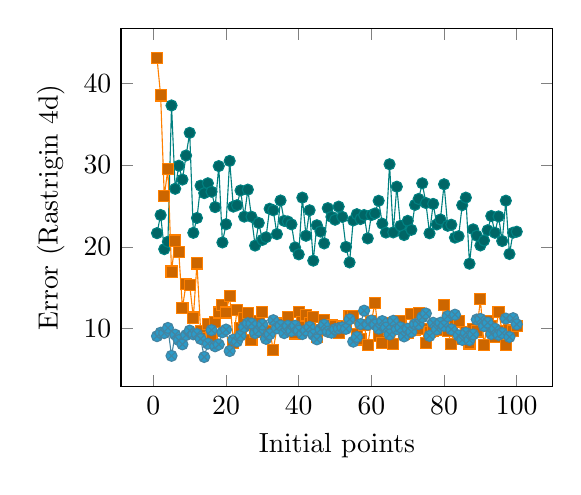
\begin{tikzpicture}
		\begin{axis}[
			xlabel = Initial points,
			ylabel = Error (Rastrigin 4d),
			cycle list name=exotic,
			legend style={at={(1.03,0.5)},anchor=west},
			scale=0.8,
			%ymode=log,
			]
			
			\addplot coordinates
			{(1,21.67791372747394)(2,23.894086481943805)(3,19.72621994504626)(4,20.62225145306321)(5,37.2767549991017)(6,27.098989271353183)(7,29.919048932963754)(8,28.22295711448973)(9,31.16347517399415)(10,33.93416058476988)(11,21.71818019521783)(12,23.530048027779912)(13,27.479885317853757)(14,26.5707269674785)(15,27.767103949188595)(16,26.742402291643486)(17,24.85950970798451)(18,29.869048359890662)(19,20.54157619090352)(20,22.76557075928751)(21,30.503832588833138)(22,24.917981338949563)(23,25.086707756165925)(24,26.898616643916984)(25,23.696403799233774)(26,26.993769966440727)(27,23.68301826666557)(28,20.160578670369766)(29,22.926812750044313)(30,20.854165831200536)(31,21.16730200504162)(32,24.65624896575979)(33,24.47276051330279)(34,21.563500550004864)(35,25.665255117918825)(36,23.178423849187208)(37,23.103810421784225)(38,22.754982975225204)(39,19.93462107276941)(40,19.087521869643815)(41,26.01679493839557)(42,21.359571485359794)(43,24.470418139479577)(44,18.317339090957613)(45,22.644783366354964)(46,21.87034775986445)(47,20.42224089881966)(48,24.729692189286432)(49,23.678590516293728)(50,23.317846054971128)(51,24.918170992587555)(52,23.664245256831084)(53,19.994224053360004)(54,18.10141548597324)(55,23.233903785678343)(56,23.990696916040708)(57,23.40085625818036)(58,23.887332326052388)(59,21.03771898451894)(60,23.886140547152102)(61,24.084553634083555)(62,25.632618541278667)(63,22.832110079679055)(64,21.750836511055635)(65,30.09306510162215)(66,21.76838450594331)(67,27.355344358806736)(68,22.57318709986254)(69,21.447149240690283)(70,23.179576513584113)(71,22.083108688365662)(72,25.12944369743228)(73,25.856128220720848)(74,27.76815237138826)(75,25.357139085446924)(76,21.659721159211713)(77,25.251107889128892)(78,22.738749510296422)(79,23.343611858165307)(80,27.651211723572782)(81,22.582382741104524)(82,22.70726955666277)(83,21.131574697662646)(84,21.30709713495851)(85,25.097895494944936)(86,26.01796081972005)(87,17.945598653970467)(88,22.143892153562554)(89,21.373410725178186)(90,20.177675261833876)(91,20.77623359457072)(92,22.034881103082075)(93,23.769230552431402)(94,21.723505500210123)(95,23.722985736002705)(96,20.716970145975555)(97,25.645331677362748)(98,19.130669992517646)(99,21.737400035085027)(100,21.855260566692507)}
			;
			
			\addplot coordinates 
			{(1,43.05801713062421)(2,38.50048156977909)(3,26.235839867859504)(4,29.48622821817756)(5,16.98988101296374)(6,20.776908999219476)(7,19.327944446722263)(8,12.526128563066095)(9,15.505367273101026)(10,15.365682044483426)(11,11.368711303601454)(12,17.97539550357209)(13,9.757094311229128)(14,8.865836070700816)(15,10.552426985250197)(16,8.942786731037367)(17,10.855212725190082)(18,11.987368644829617)(19,12.86865054244681)(20,11.985987559589592)(21,13.980035863329906)(22,8.277130509073746)(23,12.32946435467984)(24,10.046353245640628)(25,11.311350401726566)(26,11.971508505924902)(27,8.660523429267588)(28,9.611697633167648)(29,10.936736000116209)(30,12.039700942081378)(31,9.429737364679408)(32,9.770576327192696)(33,7.42889955483606)(34,10.0894975830751)(35,10.671728470193225)(36,10.589520559925365)(37,11.446021455808197)(38,9.888434471641222)(39,9.431347596757742)(40,12.094660264806853)(41,10.861501891447322)(42,11.622702340156176)(43,10.732842987228306)(44,11.440559428173543)(45,9.008827910494428)(46,9.830360727163924)(47,11.120516942629298)(48,9.954295332378729)(49,10.483515938611118)(50,10.281273085085635)(51,9.459734157042552)(52,10.25851861476485)(53,10.37605450368534)(54,11.580646902895845)(55,11.544054102666317)(56,9.335963715326159)(57,8.69552908617808)(58,10.482545347886793)(59,7.989421128205322)(60,10.888355840664934)(61,13.19584988001069)(62,9.089415575607983)(63,8.29586456078106)(64,10.647267271326392)(65,9.917271119965168)(66,8.110339087947283)(67,10.13770342715544)(68,10.921724622116349)(69,9.354285666473437)(70,9.449808321562701)(71,11.765676678372353)(72,9.91098306936228)(73,11.868159985970127)(74,9.970587134790216)(75,8.307603617517165)(76,9.612811562757317)(77,9.749288410366812)(78,9.835975004906896)(79,10.232122257060658)(80,12.861945368999113)(81,9.766824407295346)(82,8.09559132456854)(83,10.874750775312616)(84,10.926842908807888)(85,8.795378926331376)(86,9.638111133422427)(87,8.198189559233128)(88,9.926999272151189)(89,9.670965743710958)(90,13.585692487357694)(91,7.9978264032937805)(92,10.922203506102045)(93,10.359894532830722)(94,8.961911012069958)(95,12.035934347494626)(96,9.744988825078574)(97,8.043804622094985)(98,9.808666674827927)(99,9.716558463841228)(100,10.30224445231394)}
			;
			
			\addplot coordinates
			{(1,9.095857143798778)(2,9.523241549046418)(3,9.467852775414437)(4,10.101679918810904)(5,6.693820002868594)(6,9.279285532338099)(7,8.616554793530229)(8,8.099075883327618)(9,9.231421085893933)(10,9.776490121400336)(11,9.320035826340611)(12,9.344177982539176)(13,8.764631533186066)(14,6.5530432440113415)(15,8.17530035426785)(16,9.832938880370447)(17,7.8579876385949365)(18,8.084554256947063)(19,9.574357575059224)(20,9.90329812722676)(21,7.279418208504846)(22,8.664978889759611)(23,8.448823146105052)(24,9.157651301495827)(25,10.22177021554883)(26,10.674887571201463)(27,10.643022501703399)(28,9.473254156173805)(29,9.760686210234033)(30,10.509039413516122)(31,8.769821422034019)(32,9.334534467748734)(33,11.044167193024752)(34,10.063782237769011)(35,10.391727140795192)(36,9.467776070612953)(37,10.36141294257546)(38,9.720559282007295)(39,10.361718287760606)(40,9.773613054345049)(41,9.352497251782527)(42,9.81260216244038)(43,10.232714520098025)(44,9.277541652130777)(45,8.706278604221641)(46,9.938054470200942)(47,10.489322168730968)(48,9.630613884311492)(49,9.514697397254722)(50,9.95676158760241)(51,10.04640968013643)(52,10.163234642720484)(53,9.990459337096175)(54,11.15250164552299)(55,8.424238781286546)(56,8.993693706815845)(57,10.569263535788782)(58,12.211447945720852)(59,10.50704504283792)(60,10.996865520680197)(61,10.494041369600138)(62,10.016283184471504)(63,10.93251149662097)(64,10.142286447169429)(65,9.306633739556633)(66,10.967358394867485)(67,9.941449376418609)(68,10.171517692963683)(69,9.064468561944215)(70,10.001613479377596)(71,9.633742287766152)(72,10.548939995249373)(73,10.566860182441028)(74,11.415863915388897)(75,11.867683858166298)(76,9.125667657339768)(77,10.731875702973749)(78,9.915888203464402)(79,10.736593422183116)(80,10.358673232148409)(81,11.530319184105295)(82,9.928950532557167)(83,11.721208725194446)(84,9.188776957900568)(85,8.643247267585057)(86,9.498350872529082)(87,8.612601329962754)(88,9.307927272628433)(89,11.131993790623083)(90,11.202134926376994)(91,10.331187581547292)(92,10.747096469912856)(93,9.357927703196143)(94,10.009334371498639)(95,9.261897397089301)(96,9.471485460237494)(97,11.240386201697287)(98,8.995411781472653)(99,11.290842283506015)(100,10.54623277447077)}
			;
			
			
			
		\end{axis}
	\end{tikzpicture}
	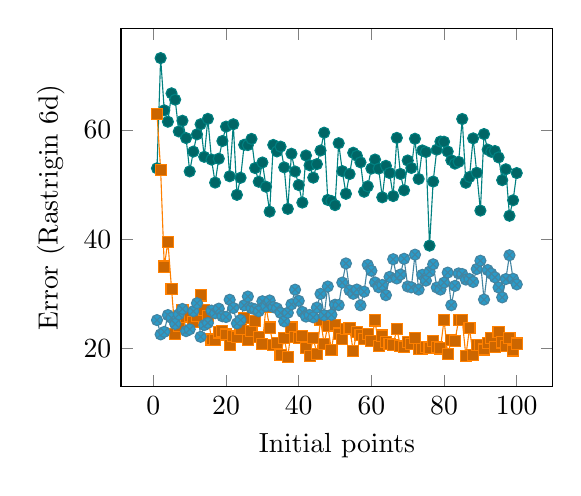
\begin{tikzpicture}
		\begin{axis}[
			xlabel = Initial points,
			ylabel = Error (Rastrigin 6d),
			cycle list name=exotic,
			legend style={at={(1.03,0.5)},anchor=west},
			scale=0.8,
			%ymode=log,
			]
			
			\addplot coordinates
			{(1,52.976304442604274)(2,73.15594543843355)(3,63.596394564210165)(4,61.51012312749496)(5,66.70811656291622)(6,65.54801268482959)(7,59.72618591919941)(8,61.6858369770114)(9,58.515278758692695)(10,52.4088932375959)(11,56.037459796336385)(12,59.19603653238064)(13,61.04389400001884)(14,55.08034564896544)(15,62.03112575515928)(16,54.575969467991875)(17,50.359840945375495)(18,54.731293390407245)(19,57.97540872647367)(20,60.61183026468795)(21,51.51932423181637)(22,61.04159614313473)(23,48.11461254522745)(24,51.24487335356066)(25,57.285695601429644)(26,57.229088047923085)(27,58.35858847807894)(28,53.02099389363517)(29,50.51308408535452)(30,54.042427546694526)(31,49.604877846585154)(32,45.04571167475526)(33,57.25812106872968)(34,56.068251938039865)(35,56.94882357854094)(36,53.14940324645361)(37,45.54617939217512)(38,55.64613596783473)(39,52.395565664013624)(40,49.90769271023531)(41,46.69877704503943)(42,55.32195832694956)(43,53.531131315395314)(44,51.26586049279278)(45,53.74306715625046)(46,56.232448146956735)(47,59.49829842127375)(48,47.18655866834751)(49,46.983077987847786)(50,46.23329341595214)(51,57.57358942181837)(52,52.45822805392792)(53,48.30825246820894)(54,51.932055254867706)(55,55.82519925313155)(56,55.28874827297538)(57,54.077858277520285)(58,48.68439440112185)(59,49.67230619914257)(60,52.93688886765223)(61,54.58238155036621)(62,52.92124512445287)(63,47.66387219414649)(64,53.429752386590074)(65,52.11829611206267)(66,47.893610203091875)(67,58.547666417364134)(68,51.94525590318663)(69,48.9504626940337)(70,54.40753962315174)(71,53.041830606980646)(72,58.386823494981)(73,51.025948275594615)(74,56.25080772303245)(75,55.96717770689703)(76,38.81587663296989)(77,50.55215451558351)(78,56.39302724954389)(79,57.87083411603718)(80,57.839989015046264)(81,56.05405491788101)(82,54.4506521700702)(83,53.83403257959385)(84,54.15489563567244)(85,62.00366658066914)(86,50.32988078728308)(87,51.39040590640957)(88,58.45879117739695)(89,52.152411783496255)(90,45.235946242899544)(91,59.24971978091817)(92,56.40529455056084)(93,56.00739693072465)(94,56.139197085276145)(95,54.97776567368014)(96,50.80765657980099)(97,52.803155085608594)(98,44.28858867454408)(99,47.120002211977955)(100,52.104356333669365)}
			;
			
			\addplot coordinates 
			{(1,62.92836760933335)(2,52.722469580550786)(3,34.99215586268427)(4,39.5333422223052)(5,30.90211733879364)(6,22.638020470092147)(7,24.074586245466023)(8,27.011110998649325)(9,25.831934376075584)(10,25.992948616043595)(11,24.89226955355592)(12,25.937757223823137)(13,29.69337352186785)(14,26.959506949137243)(15,25.9836125755535)(16,21.628583167496586)(17,21.622668136687047)(18,22.91799027972251)(19,23.177962303976212)(20,22.546097216001634)(21,20.58366926663628)(22,22.203931526214657)(23,22.1289285131423)(24,23.482571696941203)(25,25.54599343860702)(26,21.612053505592584)(27,23.251384835095802)(28,24.953468056552925)(29,22.013152691357295)(30,20.806890402724576)(31,27.61966974316195)(32,23.80996464369578)(33,20.68182292244918)(34,20.973768686810864)(35,18.796434989332198)(36,21.83751341719749)(37,18.423155139609513)(38,23.82110899356869)(39,22.0134980310561)(40,21.949392027948228)(41,22.25743168995828)(42,20.104918112940908)(43,18.624602979736057)(44,21.889076936059087)(45,18.99773956701073)(46,25.25229714280522)(47,20.810258631256193)(48,24.121952604347122)(49,19.643966587675596)(50,24.213364529153388)(51,22.719117959143652)(52,21.666872026808512)(53,23.55504981995877)(54,23.697057754663817)(55,19.570638481881836)(56,23.03219488608874)(57,22.433978413837007)(58,21.71146562349311)(59,22.672366810100876)(60,21.303792751903675)(61,25.118736513045686)(62,20.363519655282442)(63,22.344660159565887)(64,21.220193422800197)(65,20.805730906890908)(66,20.671789307509645)(67,23.535405973668468)(68,20.435508008243776)(69,20.25817637864615)(70,21.104830509690036)(71,20.837964462187557)(72,21.950260823762783)(73,19.8483334932545)(74,19.905618887441932)(75,20.298251130936926)(76,20.090095990642414)(77,21.40846385715296)(78,20.200361173537743)(79,19.992934100618164)(80,25.264926527078465)(81,18.931329792180755)(82,21.476505953965347)(83,21.411637375697147)(84,25.175095338251673)(85,25.176656838316426)(86,18.618541580059674)(87,23.68248434511426)(88,18.78015683505218)(89,20.64240327350998)(90,20.61545747586206)(91,19.79600110326711)(92,21.045979208818512)(93,21.926309966141087)(94,20.210864388808332)(95,22.985639649567354)(96,21.08690354997094)(97,20.424450264867186)(98,21.842116664216245)(99,19.616421675280222)(100,20.88712027688731)}
			;
			
			\addplot coordinates
			{(1,25.178065945336193)(2,22.5612977870603)(3,23.025711884074354)(4,26.101454952472928)(5,25.592289553694417)(6,24.47973037392388)(7,26.232257089624273)(8,27.223381868555215)(9,23.157906766046708)(10,23.49207153879888)(11,26.8111724761013)(12,28.278438888667047)(13,22.12013861021534)(14,24.261601807169598)(15,24.66897569960631)(16,26.922116781632166)(17,26.450169983708236)(18,27.27936568568638)(19,25.881141157350946)(20,25.745236228376324)(21,28.905072061285658)(22,27.402000167162917)(23,24.576960066332894)(24,25.196244077595082)(25,27.89774162719031)(26,29.496441639897192)(27,27.36465271129842)(28,27.14945317383594)(29,26.804126687985786)(30,28.629876569164566)(31,27.749651308910206)(32,28.779005037925987)(33,27.5635890203234)(34,27.330500214182983)(35,26.511432736825952)(36,24.957083434447828)(37,26.52204523789563)(38,28.06615895338975)(39,30.752709335638578)(40,28.70604063088507)(41,26.66773473888764)(42,25.82241510135528)(43,26.12257402023418)(44,25.69240655820562)(45,27.47783013903678)(46,29.98388463866389)(47,26.071758508596776)(48,31.335186683778925)(49,26.16053333872869)(50,27.999993340278433)(51,27.93307983551432)(52,32.0551630658975)(53,35.55850120636076)(54,30.620601166149537)(55,29.998372675845495)(56,30.77595720942125)(57,27.881902722519612)(58,30.385888760356618)(59,35.27976270508966)(60,34.21315535903018)(61,32.08443938970416)(62,31.195465119251935)(63,31.61905500273226)(64,29.742620239347865)(65,33.08717024996183)(66,36.327031677535885)(67,32.80247019729241)(68,33.52530121948264)(69,36.4073823424251)(70,31.336673967917847)(71,31.17436179976021)(72,37.16646574596194)(73,30.767555270124774)(74,33.47246842427124)(75,32.40663189479692)(76,34.05808741962967)(77,35.39907292662392)(78,31.147300090994406)(79,30.76550773414693)(80,32.05078899401576)(81,33.87586822016051)(82,27.909473955836983)(83,31.448224518469534)(84,33.73426265156324)(85,33.616704187360014)(86,32.595599609531604)(87,32.70196279620684)(88,32.16615211970232)(89,34.54039434923287)(90,36.053835243123345)(91,28.939820280400994)(92,34.353847804859335)(93,33.68907222910764)(94,33.010088745807565)(95,31.153588287738803)(96,29.34380166719033)(97,32.69283356167121)(98,37.05990034396095)(99,32.73578587525532)(100,31.722247648006277)}
			;
			
			
			
		\end{axis}
	\end{tikzpicture}
	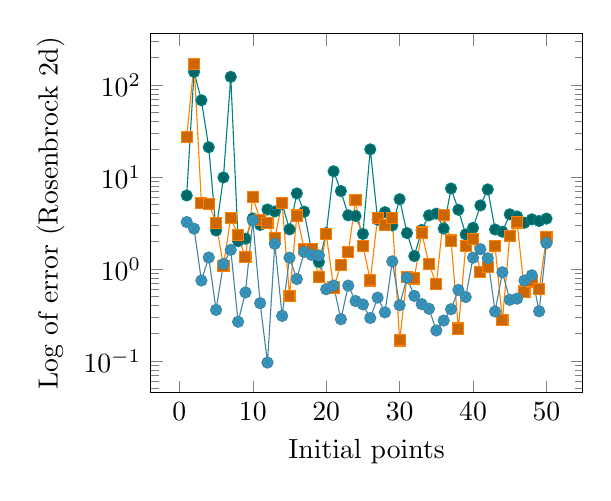
\begin{tikzpicture}
		\begin{axis}[
			xlabel = Initial points,
			ylabel = Log of error (Rosenbrock 2d),
			cycle list name=exotic,
			legend style={at={(1.03,0.5)},anchor=west},
			scale=0.8,
			ymode=log,
			]
			
			\addplot coordinates
			{(1,6.292806616493855)(2,138.91038976388086)(3,68.29395518155609)(4,21.068014337508338)(5,2.620834053060887)(6,9.888782157610109)(7,122.80835248582272)(8,2.0043901313861907)(9,2.13116963848453)(10,3.5444779890656593)(11,3.0141472673423406)(12,4.4338142600937305)(13,4.222000928315547)(14,5.087787618104964)(15,2.6952261585179813)(16,6.629643666983215)(17,4.198970560725005)(18,1.568868862303444)(19,1.1911686993689676)(20,2.461106460294555)(21,11.54538363088382)(22,7.031423596842529)(23,3.833020345575938)(24,3.7689493164214647)(25,2.4014751295140564)(26,19.991194467093074)(27,3.4374121783742972)(28,4.144689086932063)(29,2.976677384600417)(30,5.737788295879791)(31,2.4559670048347018)(32,1.3817586817854015)(33,2.6534375813528266)(34,3.8256745545208175)(35,3.995255793878564)(36,2.7505744654026936)(37,7.503826821755996)(38,4.401079292919496)(39,2.3755603375231384)(40,2.8000259532012173)(41,4.907844915498686)(42,7.3310887628242964)(43,2.686280444756032)(44,2.540925955374987)(45,3.930574692737595)(46,3.725223029284097)(47,3.179491893862133)(48,3.4625118730423603)(49,3.324396024198104)(50,3.526034690975181)}
			;
			
			\addplot coordinates 
			{(1,27.165820171340357)(2,170.54170701401708)(3,5.224800559316149)(4,5.098695780505748)(5,3.1893716640068623)(6,1.0805384730616117)(7,3.6056400766990016)(8,2.31816873384094)(9,1.3360460440799136)(10,6.047127519304739)(11,3.414063965455366)(12,3.1287415807338284)(13,2.1844932107787582)(14,5.234262991759788)(15,0.5052161018714074)(16,3.8108123159356055)(17,1.6602110398770393)(18,1.6298415204212062)(19,0.8237530497770216)(20,2.4116947024497843)(21,0.627926002990301)(22,1.1016005404689664)(23,1.521476230433978)(24,5.565285142738238)(25,1.7955306721924784)(26,0.7504656448092601)(27,3.6189554690552654)(28,2.995172843123591)(29,3.6057829902776724)(30,0.16699032003246517)(31,0.8260687649410325)(32,0.7883694305692158)(33,2.4882095711307755)(34,1.1376213535011106)(35,0.6801757527577168)(36,3.8402513748095837)(37,2.036278678981804)(38,0.22497573091233308)(39,1.7729898875476526)(40,2.126043385087983)(41,0.9343450797802146)(42,1.0565380935728217)(43,1.7704782774944374)(44,0.2775665834019284)(45,2.2810821548101097)(46,3.2044563690981542)(47,0.5677113996015085)(48,0.7305795245016778)(49,0.6001944314361027)(50,2.220905761425119)}
			;
			
			\addplot coordinates
			{(1,3.2349360883746017)(2,2.7428314042694306)(3,0.7489467374587943)(4,1.331608204376738)(5,0.3587451831910896)(6,1.1341819888255993)(7,1.613193369256286)(8,0.26647989095683117)(9,0.5555377027046497)(10,3.3729628265990437)(11,0.42469142230293466)(12,0.09589074863026274)(13,1.876536171121718)(14,0.30887399239408525)(15,1.326778517363644)(16,0.7766942053081306)(17,1.5330966984710084)(18,1.4242085808625056)(19,1.403014041681105)(20,0.6011422091306245)(21,0.6599450138819608)(22,0.2841542836857282)(23,0.6591608432530882)(24,0.44777896802988587)(25,0.41117287635331945)(26,0.2926660428315085)(27,0.48776330631647075)(28,0.3371792425255456)(29,1.2095891045646483)(30,0.4032046794433929)(31,0.8022347586771084)(32,0.5094435133362806)(33,0.4153134088825886)(34,0.3692048401669542)(35,0.2143873503118463)(36,0.27460992822323094)(37,0.36507043199308903)(38,0.5917435473413785)(39,0.4954453027105946)(40,1.3252404682130254)(41,1.6407754232654903)(42,1.3049827190764014)(43,0.34456141654903144)(44,0.9205776951863704)(45,0.4619262988222078)(46,0.4758816169124418)(47,0.7482822470897819)(48,0.8531471016295169)(49,0.34678666954091814)(50,1.9146566005251457)}
			;
			
			
			%\legend{Strategy 1, Strategy 2, Strategy 3}
			
		\end{axis}
	\end{tikzpicture}
	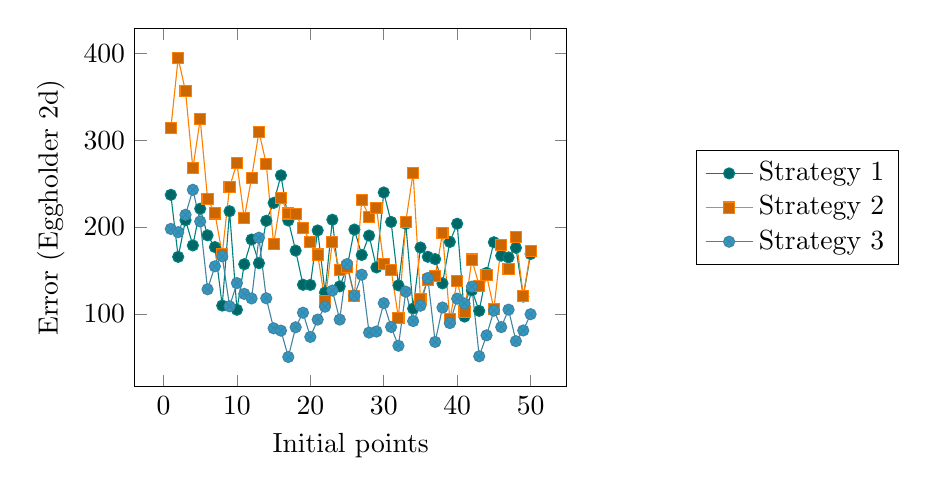
\begin{tikzpicture}
	\begin{axis}[
		xlabel = Initial points,
		ylabel = Error (Eggholder 2d),
		cycle list name=exotic,
		legend style={at={(1.3,0.5)},anchor=west},
		scale=0.8,
		%ymode=log,
		]
		
		\addplot coordinates
		{(1,237.05147354720629)(2,165.67376382303573)(3,207.89427437056588)(4,178.85209553453333)(5,221.09858891030336)(6,190.44688117871942)(7,176.937479240219)(8,109.61769501400386)(9,218.17501771632405)(10,104.80893245593006)(11,157.21238234901526)(12,185.6215442585413)(13,158.42432852406537)(14,207.19674407758674)(15,227.7681552465164)(16,259.48266564246876)(17,207.49941290123124)(18,172.85951300639044)(19,133.59498835825144)(20,133.3909964076269)(21,196.0591227401475)(22,124.72361624694165)(23,208.4123258195804)(24,131.7109460633868)(25,153.32063025450844)(26,197.09750649815032)(27,167.8305711685407)(28,190.13549763914725)(29,153.4883275666416)(30,239.7816275244109)(31,205.85517668112107)(32,132.86704378991735)(33,203.76897160484828)(34,106.2028046530052)(35,176.44259359252882)(36,165.7827006437404)(37,163.10674595919258)(38,135.16988527632907)(39,182.84033313751192)(40,203.79983800369897)(41,96.93286913383415)(42,127.11819316632167)(43,103.50577555862279)(44,147.21982984444202)(45,182.48229659784155)(46,167.0366793613104)(47,165.05617364079717)(48,176.08176609779048)(49,119.98976220221701)(50,169.00863400365483)}
		;
		
		\addplot coordinates 
		{(1,313.54139274152203)(2,394.373925709319)(3,356.09675282171315)(4,267.5158343951515)(5,324.03641097684897)(6,232.69746908540046)(7,215.66742900345702)(8,168.89932571570165)(9,246.05408452755518)(10,273.33085690751045)(11,210.23051810477568)(12,256.69181075410216)(13,309.6799905932031)(14,272.71748421394716)(15,180.06045624424843)(16,233.3533730107054)(17,215.56421717944028)(18,214.57678595998928)(19,198.54768153593162)(20,183.17866624939631)(21,168.34260804994042)(22,114.34399631110507)(23,182.89608027564378)(24,150.20305048934375)(25,154.4505266065417)(26,120.85610942792866)(27,231.38976395511978)(28,211.4049912013209)(29,222.04874700388592)(30,157.50340435737735)(31,151.0011460865316)(32,95.16222473767719)(33,206.1413168924218)(34,262.354321085651)(35,116.91110823445752)(36,138.94619235534725)(37,143.41984487905523)(38,192.81717173027906)(39,94.18370851084492)(40,137.56290169719483)(41,102.72810094214981)(42,162.58389038097226)(43,132.5305018351546)(44,144.48093592104738)(45,105.87430854199583)(46,179.26104969026295)(47,151.75905358558038)(48,188.4767428253761)(49,120.8786744216624)(50,172.00361719657317)}
		;
		
		\addplot coordinates
		{(1,197.81757874441573)(2,194.0937702392151)(3,214.09256062925533)(4,242.84656884796468)(5,206.40299187081365)(6,128.39962476083718)(7,154.75960154154436)(8,166.2652111351925)(9,108.78508310974617)(10,135.45515406185956)(11,123.08885808788719)(12,117.83408554772654)(13,187.6727644608912)(14,118.01655745823909)(15,83.47940158552)(16,80.76091289280504)(17,50.46993985925277)(18,84.63983475137235)(19,101.41342502253339)(20,73.55540985277)(21,93.4748991090739)(22,108.32429590304059)(23,126.90017585247392)(24,93.51544902941978)(25,157.34935646034)(26,121.02466610028823)(27,145.14580070912453)(28,78.501947262262)(29,79.77287520494285)(30,112.42532948884397)(31,85.02544435162551)(32,63.3269663868866)(33,125.6420829343634)(34,91.78404241689988)(35,109.48756786508802)(36,141.3441101499843)(37,67.80979210153941)(38,107.380858765915)(39,89.44792095658406)(40,117.54642599977242)(41,112.07167608689456)(42,131.40070798594633)(43,51.26223041389424)(44,75.36649422789937)(45,103.793064453413)(46,84.83854024914606)(47,104.93508872349157)(48,68.67120900272894)(49,80.98933743080525)(50,99.71400296415234)}
		;
		
		
		\legend{Strategy 1, Strategy 2, Strategy 3}
		
		\end{axis}
	\end{tikzpicture}
	\caption{ Error of the optimum found by the algorithm depending on the number of initial points. The budget is 200 in all two dimensional cases and 400 in the 4- and 6-dimensional problem. Each point is the average of 10 evaluations. }	
	\label{fig:init_points_alternatives}
\end{figure}

For the Rastrigin function, the problem was solved for two (Figure \ref{fig:init_points_alternatives}, top left), four (Figure \ref{fig:init_points_alternatives}, top right), and six  (Figure \ref{fig:init_points_alternatives}, center left) dimensions. In all three cases, similar behavior can be observed for each refinement strategy. For the first algorithm, the error decreases with increasing number of initial points. This is the same for the second strategy but with the difference that it is increasing much faster and seems to be saturated with a sufficiently high number of initial points. For strategy 3, a lower value compared to the other strategies results in smaller errors of the optimum. As depicted in the upper left plot, a minimal number is also not perfect for this parameter. Good results are achieved with 5 to 15 initial points for the two-dimensional case. 

For the Rosenbrock and Eggholder function, the behavior is the same for all alternative refinement strategies. The error decreases with a higher number of initial points. Note that these two test functions are very hard to optimize and a generally high number of function evaluations would lead to better results. In this case, the budget was only 200. \newline 

For the behavior on the Rastrigin function, we can conclude that strategy 1 is not the best because the results are getting better when the number of refinements decreases. This means that the algorithm is not performing well. The results for the second and third refinement strategies are very promising as they perform well already for a small number of initial points which means that the refinements are finding good optima. \newline 

We can conclude that for higher dimension, higher number of initial points works best for strategy 1 and strategy 2.



\subsubsection{Number of refinements per iteration}

The next parameter that is influencing the performance of the algorithm is the number of refinements per iteration. Intuitively, a higher value for this parameter makes the algorithm less adaptive because the point that has to be refined is chosen fewer times. To analyze this parameter, again the three functions (Rastrigin in 2, 4, and 6 dimensions and Rosenbrock and Eggholder in 2 dimensions) are optimized with a budget of 200 in the case of the 2-d problems and 400 for 4 and 6 dimensions. The resulting errors which are the averages of ten runs with up to 50 refinements per iteration are presented in Figure \ref{fig:ref_per_step}. The adaptivity parameters are set as in the previous experiment where the number of initial points is analyzed. \newline 

\begin{figure}[H]
	\centering
	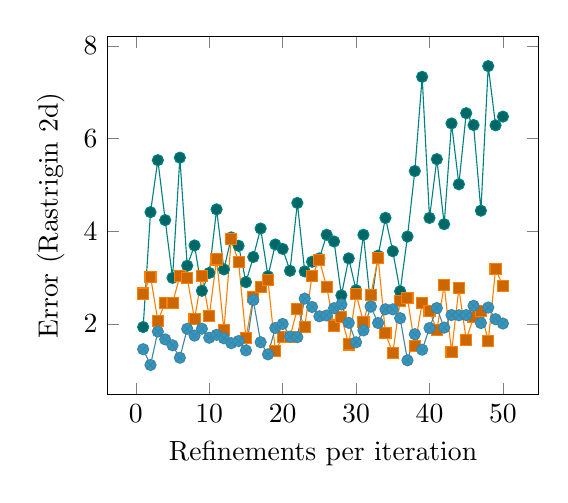
\begin{tikzpicture}
		\begin{axis}[
			xlabel = Refinements per iteration,
			ylabel = Error (Rastrigin 2d),
			cycle list name=exotic,
			legend style={at={(1.03,0.5)},anchor=west},
			scale=0.8,
			%ymode=log,
			]
			
			\addplot coordinates
			{(1,1.9299573510344796)(2,4.409640365457989)(3,5.531364135438023)(4,4.237506421116211)(5,2.9914288403429703)(6,5.586122500353136)(7,3.2531270945290864)(8,3.6914574953729344)(9,2.712425743033958)(10,3.097681109230355)(11,4.470109336523421)(12,3.173844761960128)(13,3.8645153959777985)(14,3.684303376685358)(15,2.89884126843918)(16,3.4417379054105552)(17,4.056957591091863)(18,3.025951967877651)(19,3.711936711668689)(20,3.6168401198098694)(21,3.1437879829570194)(22,4.608252841366175)(23,3.130402943357308)(24,3.3397601865146553)(25,3.4117946040801135)(26,3.921098652941224)(27,3.7767209099735313)(28,2.6138437074378205)(29,3.412287948489772)(30,2.724233552866161)(31,3.921693249507374)(32,2.3743564428927946)(33,3.4698904509127955)(34,4.286577055606292)(35,3.5661885184514994)(36,2.702381121152052)(37,3.883340228314161)(38,5.297073199121861)(39,7.33010620843591)(40,4.28539643196596)(41,5.552833978496482)(42,4.150452735757783)(43,6.324167896807491)(44,5.011169035621856)(45,6.545573106214991)(46,6.289816909094339)(47,4.4417189116903275)(48,7.561718182649079)(49,6.2834545904366355)(50,6.471949896346198)}
			;
			
			\addplot coordinates 
			{(1,2.6529179650826626)(2,3.018366306145631)(3,2.066239171003123)(4,2.45328321939673)(5,2.445261939084422)(6,3.033358293902926)(7,2.989617994090822)(8,2.0978989416628284)(9,3.0249575180252752)(10,2.163645677272489)(11,3.3882908106236416)(12,1.867354235100514)(13,3.8230575649174154)(14,3.328885267419514)(15,1.6898994866099102)(16,2.582171593035887)(17,2.8027292652798366)(18,2.9382587614328655)(19,1.421438954023083)(20,1.7122662902372063)(21,1.7188684745275773)(22,2.3210417091324334)(23,1.936236776519398)(24,3.03423684215631)(25,3.3710942780066198)(26,2.791525485452614)(27,1.9621756204174836)(28,2.146809854786066)(29,1.5541296904631487)(30,2.6460021702031145)(31,2.040365484114894)(32,2.6190194364371147)(33,3.4257510252342227)(34,1.7939648058998272)(35,1.3690550482606194)(36,2.4940110478286743)(37,2.558152079651511)(38,1.5272866752300218)(39,2.4418833425812805)(40,2.2797788085503923)(41,1.8672639237120863)(42,2.8340557594544915)(43,1.389657002265368)(44,2.7649287473659236)(45,1.657612693585452)(46,2.140140071156882)(47,2.2795739563328743)(48,1.6236202742866908)(49,3.1801622393809073)(50,2.817180557883542)}
			;
			
			\addplot coordinates
			{(1,1.4512769442919513)(2,1.1108279638761753)(3,1.8317607126549666)(4,1.6627799406493864)(5,1.5357973596882033)(6,1.2671728459122327)(7,1.8919863826847678)(8,1.7452373323060164)(9,1.8937731500977055)(10,1.6992179589800134)(11,1.7618431181729264)(12,1.6865474435320018)(13,1.5827003368507797)(14,1.6275393266611176)(15,1.425857403978092)(16,2.5119438894794697)(17,1.6024129277690744)(18,1.3405914595216248)(19,1.910046415346219)(20,1.997562603439676)(21,1.723531268168457)(22,1.7117709827092036)(23,2.544126967278973)(24,2.363476977639549)(25,2.161965649325704)(26,2.180380035632412)(27,2.3372716976778767)(28,2.4172372435121248)(29,2.0210054405010904)(30,1.6002325026945932)(31,1.8579084849260366)(32,2.3742640234874917)(33,2.0167008209713906)(34,2.3137401661041483)(35,2.311917538936072)(36,2.1217259019674315)(37,1.2118563503755309)(38,1.7757457528541014)(39,1.4404261553044144)(40,1.9078835568842254)(41,2.3407216516101053)(42,1.9178058349263658)(43,2.1897361635386803)(44,2.1841078824820834)(45,2.187678893096707)(46,2.3888473799539724)(47,2.0159923383007006)(48,2.3520983877063917)(49,2.099833010997215)(50,2.005936612088075)}
			;
			
			
			% \legend{Strategy 1, Strategy 2, Strategy 3}
			
		\end{axis}
	\end{tikzpicture}
	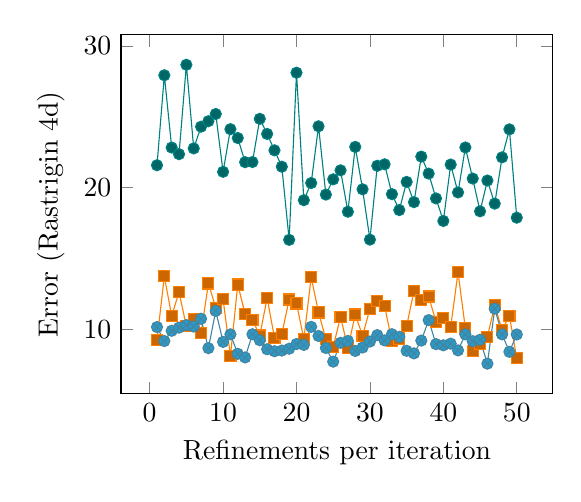
\begin{tikzpicture}
		\begin{axis}[
			xlabel = Refinements per iteration,
			ylabel = Error (Rastrigin 4d),
			cycle list name=exotic,
			legend style={at={(1.03,0.5)},anchor=west},
			scale=0.8,
			%ymode=log,
			]
			
			\addplot coordinates
			{(1,21.571450925827087)(2,27.920985744612324)(3,22.817786017257824)(4,22.35293514442489)(5,28.661029883609707)(6,22.759198399134995)(7,24.29179277188364)(8,24.680280809661944)(9,25.18768605020383)(10,21.105053547590707)(11,24.11667334367236)(12,23.49361193651392)(13,21.787647106472527)(14,21.798211231102012)(15,24.84601159359948)(16,23.780270801805464)(17,22.62560394058462)(18,21.468508620323423)(19,16.304286766760434)(20,28.102135000988376)(21,19.10348671712194)(22,20.315986522319232)(23,24.31993047159746)(24,19.498992076741313)(25,20.576132823276613)(26,21.212287960932105)(27,18.289366923243087)(28,22.865610933033416)(29,19.873478964007138)(30,16.3210794406717)(31,21.53201789485596)(32,21.636680302178963)(33,19.530470654609733)(34,18.405080643057666)(35,20.394881902261908)(36,18.96647355055265)(37,22.179759514439716)(38,20.980777919385286)(39,19.229622434366327)(40,17.63697243517336)(41,21.619072476537703)(42,19.65008932496867)(43,22.82634152931717)(44,20.62913984173121)(45,18.318526976141065)(46,20.49146076991186)(47,18.86015380464162)(48,22.12802478790763)(49,24.104174273944967)(50,17.86989806728193)}
			;
			
			\addplot coordinates 
			{(1,9.232409027301737)(2,13.735954156544304)(3,10.934313341357385)(4,12.616105224302142)(5,10.201321804777155)(6,10.711329526176161)(7,9.73222094351259)(8,13.227793485437022)(9,11.514580716244746)(10,12.106161026119873)(11,8.115121555219547)(12,13.150241926967045)(13,11.073843230530839)(14,10.655574342297587)(15,9.554689130871244)(16,12.200138275799116)(17,9.397100405687596)(18,9.665133829202158)(19,12.094647217026047)(20,11.81411777220905)(21,9.313802742558725)(22,13.667155148958992)(23,11.182052270816108)(24,9.293952560370489)(25,8.75904649277789)(26,10.87353679318036)(27,8.662659583008173)(28,11.03661260272074)(29,9.534745515969902)(30,11.440287481006013)(31,11.962128708714923)(32,11.618739693890515)(33,9.149890532763013)(34,9.33835671177356)(35,10.212142338611212)(36,12.69541276598593)(37,12.06404533416111)(38,12.305059788528444)(39,10.523726360130036)(40,10.80397418843489)(41,10.148129318757366)(42,14.022519856117516)(43,10.053373687164953)(44,8.46122235576871)(45,8.928111267317984)(46,9.461743926922331)(47,11.683277032362685)(48,9.953365584448662)(49,10.926396547581751)(50,7.958965198371433)}
			;
			
			\addplot coordinates
			{(1,10.149214314572884)(2,9.163146934343093)(3,9.886637545145767)(4,10.109245408097731)(5,10.286882391759157)(6,10.184503907574499)(7,10.734293606120293)(8,8.66107592378394)(9,11.287459738044646)(10,9.102771685728817)(11,9.635923106295216)(12,8.262586167462338)(13,8.004767399629497)(14,9.64001702157945)(15,9.219131452878539)(16,8.584087228603824)(17,8.444021690380072)(18,8.491525785061807)(19,8.62119916818063)(20,8.9505871029475)(21,8.890429746092101)(22,10.163068910680831)(23,9.522052079202789)(24,8.673604097066095)(25,7.7085242327590375)(26,9.036297594795062)(27,9.170165272649285)(28,8.464871029218475)(29,8.706524613026392)(30,9.126652469933301)(31,9.579980245636563)(32,9.207242587693267)(33,9.642649117518852)(34,9.457020781843372)(35,8.472055244581469)(36,8.292255917103095)(37,9.195869765927572)(38,10.639120743280717)(39,8.944224381861726)(40,8.860796338248491)(41,8.9780566079851)(42,8.503664004091878)(43,9.633204387241893)(44,9.151046998009932)(45,9.25524151533916)(46,7.566636501981327)(47,11.448096827739795)(48,9.633550772707439)(49,8.401742914495973)(50,9.626282519383338)}
			;
			
			
			
		\end{axis}
	\end{tikzpicture}
	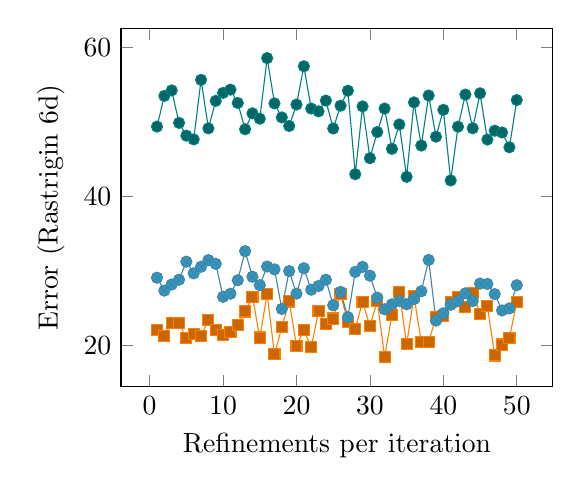
\begin{tikzpicture}
		\begin{axis}[
			xlabel = Refinements per iteration,
			ylabel = Error (Rastrigin 6d),
			cycle list name=exotic,
			legend style={at={(1.03,0.5)},anchor=west},
			scale=0.8,
			%ymode=log,
			]
			
			\addplot coordinates
			{(1,49.38591333716395)(2,53.50433748254527)(3,54.23865066035004)(4,49.88319444776785)(5,48.16944509609707)(6,47.667151716864375)(7,55.656408492619406)(8,49.1473603444771)(9,52.83236913081066)(10,53.90491965094162)(11,54.341581464572144)(12,52.55593640005368)(13,49.031828341589446)(14,51.164069894153315)(15,50.44157344797603)(16,58.569092400212426)(17,52.49561090696469)(18,50.61997478244439)(19,49.4643333490712)(20,52.339677808972695)(21,57.477643826840236)(22,51.80601930817445)(23,51.42732643610066)(24,52.870694379614974)(25,49.13443318667349)(26,52.18831512168394)(27,54.20054005930166)(28,43.00153807907424)(29,52.09724476343611)(30,45.149243018892804)(31,48.655683790512555)(32,51.80603347658689)(33,46.401919155876)(34,49.67093251210167)(35,42.64774722506638)(36,52.635499942423905)(37,46.84113126816724)(38,53.55996901782563)(39,48.02861057913469)(40,51.63505723353884)(41,42.162912087772966)(42,49.375132458955704)(43,53.67695259966283)(44,49.16223207215682)(45,53.84923646850577)(46,47.64715152683897)(47,48.83209664315923)(48,48.59452094504297)(49,46.61070620698016)(50,52.942263851191925)}
			;
			
			\addplot coordinates 
			{(1,22.070526118454072)(2,21.333058217525988)(3,23.057357200304526)(4,23.025750065793986)(5,21.011857713488574)(6,21.554647244613662)(7,21.33350641163483)(8,23.413413957611606)(9,22.060704415686043)(10,21.41817814192249)(11,21.81709196168557)(12,22.786879705760178)(13,24.59821107833885)(14,26.570794508650845)(15,21.09091250642587)(16,26.956092153953726)(17,18.85673738832668)(18,22.517506408028)(19,25.938592569991414)(20,19.98648638818647)(21,22.101047515960342)(22,19.792695047683406)(23,24.643737552881117)(24,22.891811019114208)(25,23.63702630712462)(26,26.904124412724947)(27,23.162342730800816)(28,22.282083268744547)(29,25.888346853061115)(30,22.637005720516754)(31,25.945439212320444)(32,18.486651231586322)(33,24.13019875446479)(34,27.23259701211195)(35,20.18171110482897)(36,26.636588477166207)(37,20.50603527400843)(38,20.48999205306534)(39,23.854278240279015)(40,23.96049916753388)(41,25.840470904081435)(42,26.47545755247294)(43,25.16757020001217)(44,27.090162267369255)(45,24.286840369575753)(46,25.276931023923833)(47,18.695110751968098)(48,20.15450428033849)(49,21.01389760368652)(50,25.866015985561056)}
			;
			
			\addplot coordinates
			{(1,29.122652839576595)(2,27.385483531167665)(3,28.207488587628536)(4,28.846961808486753)(5,31.269260881408872)(6,29.70590106160352)(7,30.586979278791585)(8,31.47276969303589)(9,30.974969687088453)(10,26.55865002708594)(11,26.969664822406695)(12,28.778652190764724)(13,32.685737161226655)(14,29.248711285828485)(15,28.118517735281074)(16,30.62034033041177)(17,30.242255902790276)(18,24.931541175866858)(19,30.009951775445252)(20,26.98351461262788)(21,30.3874318734345)(22,27.506301887026147)(23,28.004707233798694)(24,28.84815867515444)(25,25.42392685155604)(26,27.221866028428735)(27,23.827477974938294)(28,29.897846286564977)(29,30.568080383535523)(30,29.394435067347494)(31,26.44104240968496)(32,24.888740887220518)(33,25.54989302602406)(34,25.99224778944974)(35,25.56331715052674)(36,26.256953839568126)(37,27.30462560431988)(38,31.50236124857085)(39,23.36673303914753)(40,24.353941238765607)(41,25.49234645636335)(42,26.006274609036343)(43,27.028559557967935)(44,25.987055079939772)(45,28.33203099096334)(46,28.28261677861651)(47,26.917212390393054)(48,24.73268255833466)(49,25.001102102130663)(50,28.11421658962064)}
			;
			
			
			
		\end{axis}
	\end{tikzpicture}
	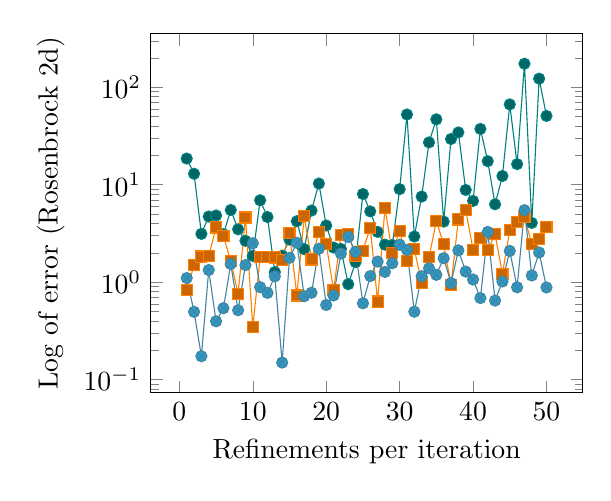
\begin{tikzpicture}
		\begin{axis}[
			xlabel = Refinements per iteration,
			ylabel = Log of error (Rosenbrock 2d),
			cycle list name=exotic,
			legend style={at={(1.03,0.5)},anchor=west},
			scale=0.8,
			ymode=log,
			]
			
			\addplot coordinates
			{(1,18.578914799361378)(2,12.966629532506198)(3,3.136345185968546)(4,4.727230618792595)(5,4.838313172173086)(6,3.111323922875184)(7,5.510496925095651)(8,3.495106865521925)(9,2.6601546103006166)(10,1.8640973073979648)(11,6.9372809644533024)(12,4.664638894677492)(13,1.271469713448353)(14,1.8735954162739135)(15,2.7357524830142843)(16,4.228730471160132)(17,2.1856605310517585)(18,5.438612153807414)(19,10.29601692101828)(20,3.8242803291902163)(21,2.2697447428536384)(22,2.194966989847775)(23,0.9551258837821839)(24,1.6087999455516584)(25,8.039879619193233)(26,5.329528346209477)(27,3.285339138157891)(28,2.4313739559041396)(29,2.408755197497834)(30,9.021141844190318)(31,52.64372216209633)(32,2.94574403517801)(33,7.5720947460188395)(34,27.203732725048734)(35,46.93870495863303)(36,4.189622667750328)(37,29.483659347395125)(38,34.45684286471187)(39,8.85321821899771)(40,6.827584965434224)(41,37.40473939205823)(42,17.457277057257215)(43,6.307588833447268)(44,12.30903548758572)(45,66.75059761244938)(46,16.289055492133922)(47,174.49648246634078)(48,4.063757876082571)(49,122.67374385239675)(50,50.86101520837304)}
			;
			
			\addplot coordinates 
			{(1,0.8301540714530692)(2,1.4963637525689288)(3,1.8348939982872903)(4,1.8679996133366088)(5,3.649118072496227)(6,2.9686537659603265)(7,1.643151548583242)(8,0.7577779355524911)(9,4.6145425041993136)(10,0.3498322234593)(11,1.8072698758530386)(12,1.8331302273624583)(13,1.7956737643414526)(14,1.705553426000683)(15,3.188574764093397)(16,0.7315054277165565)(17,4.74015856719337)(18,1.7145820807971226)(19,3.2524096518561914)(20,2.4892627246179946)(21,0.8268704474524815)(22,3.0283174591824835)(23,3.145696864199526)(24,1.8601755925966494)(25,2.111747569299978)(26,3.6312476040763153)(27,0.6335248637837501)(28,5.772898653608964)(29,1.9987074653443635)(30,3.372989543529992)(31,1.6565716743194194)(32,2.1758152801656707)(33,0.9873037253382917)(34,1.8017707435326837)(35,4.238044621411487)(36,2.4463510069171526)(37,0.935661439583046)(38,4.407608234060953)(39,5.50381814269194)(40,2.1546726079612233)(41,2.8408926272286315)(42,2.1257613257946213)(43,3.107530385874048)(44,1.2196930691637915)(45,3.4411668006308935)(46,4.116110654835701)(47,4.631216662404047)(48,2.4766942959430005)(49,2.753759422726829)(50,3.7137721827979355)}
			;
			
			\addplot coordinates
			{(1,1.104805149113282)(2,0.4972872221407182)(3,0.17418676914681458)(4,1.3347258760874467)(5,0.39771027333302345)(6,0.5420317971176106)(7,1.5397525928170832)(8,0.5163380288475172)(9,1.5000193467447172)(10,2.51234443977284)(11,0.8896387166093952)(12,0.7783738333980637)(13,1.149553848716367)(14,0.14989418672057575)(15,1.7810135120282218)(16,2.541559171223918)(17,0.7192810944077614)(18,0.7806017146208891)(19,2.2064619312859266)(20,0.5848257891414661)(21,0.7313357397432688)(22,1.970508095881522)(23,2.916681440940084)(24,2.0521404083840613)(25,0.6085482633350923)(26,1.15695903504908)(27,1.6298862926470659)(28,1.2765328803897513)(29,1.5664896650577025)(30,2.4244675221093286)(31,2.1470953447066337)(32,0.4986456556265872)(33,1.1531285384096268)(34,1.3897977823686993)(35,1.1915210894549673)(36,1.7638454159775645)(37,0.9808822009483092)(38,2.124105521700882)(39,1.285904959645777)(40,1.0664648133311139)(41,0.688180838555574)(42,3.2834295915792735)(43,0.6484067264151291)(44,1.019141966376356)(45,2.096917749105889)(46,0.8878155534709343)(47,5.485393555023345)(48,1.172941032899591)(49,2.0208413860179113)(50,0.8844246647950254)}
			;
			
			
			%\legend{Strategy 1, Strategy 2, Strategy 3}
			
		\end{axis}
	\end{tikzpicture}
	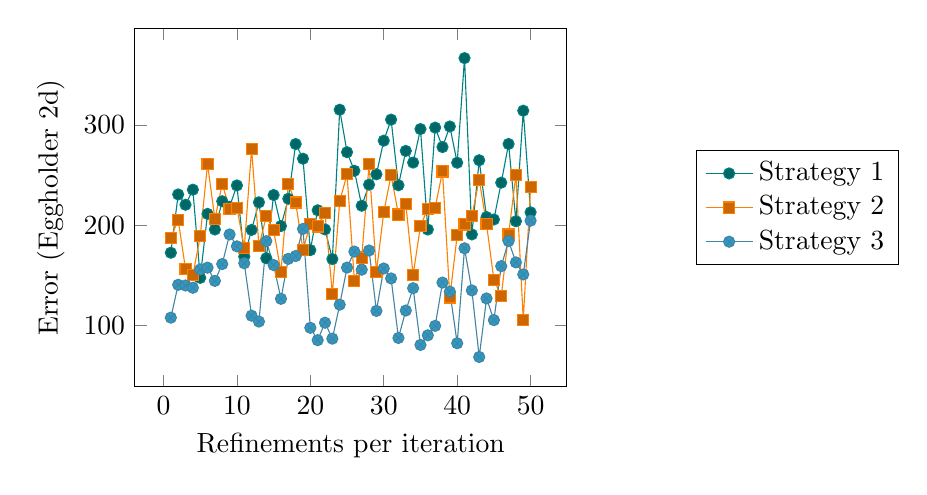
\begin{tikzpicture}
		\begin{axis}[
			xlabel = Refinements per iteration,
			ylabel = Error (Eggholder 2d),
			cycle list name=exotic,
			legend style={at={(1.3,0.5)},anchor=west},
			scale=0.8,
			%ymode=log,
			]
			
			\addplot coordinates
			{(1,172.5294175335598)(2,230.65620528276457)(3,220.35149218635064)(4,235.42782346025962)(5,147.48701538532936)(6,211.27563977123054)(7,195.6711545681204)(8,223.87404474566665)(9,218.36042884936168)(10,239.64045818284293)(11,168.78631675893126)(12,195.30263051353694)(13,222.81035195909197)(14,167.03259939937575)(15,230.08221323049688)(16,199.15199329966276)(17,226.35453302655114)(18,280.88120647383585)(19,266.2797773006218)(20,175.1605235479771)(21,214.86619357788587)(22,195.77418800833917)(23,166.2406391912569)(24,315.12483199953533)(25,272.77670714370436)(26,254.24835820230928)(27,219.36916240998465)(28,240.37522163213208)(29,250.7304541704826)(30,284.27814005091096)(31,305.2307901618818)(32,239.79344471470282)(33,274.0509126127127)(34,262.40332121187487)(35,295.82003560879195)(36,195.6694119564502)(37,297.27986800129)(38,277.8973263536667)(39,298.4189103530505)(40,262.26687676280216)(41,366.56058961432706)(42,190.78159479701145)(43,264.7386251907196)(44,208.06943802682227)(45,205.67803033784716)(46,242.38453481383058)(47,280.95401625275315)(48,203.95169586920503)(49,314.15760682072437)(50,212.82464013255407)}
			;
			
			\addplot coordinates 
			{(1,187.42160762598527)(2,205.10098203246122)(3,156.37190468280446)(4,150.28460942081665)(5,188.91369194615203)(6,261.11980237337957)(7,206.06357857268827)(8,241.2714375302832)(9,216.12461769495766)(10,217.53781910928714)(11,177.35445587379849)(12,276.07201646709206)(13,179.42073898134404)(14,208.74780595992343)(15,195.25707117187122)(16,153.35707299172017)(17,240.7999075094257)(18,222.62190282546877)(19,175.55747215741167)(20,201.16857477050078)(21,198.71931231305857)(22,211.74551983666606)(23,131.7106131557855)(24,223.8711289234151)(25,250.73669377301957)(26,144.69653458681697)(27,167.71831627547823)(28,260.83748664989264)(29,153.33675649378569)(30,212.91600144845324)(31,250.00939062745852)(32,210.57650898653938)(33,221.32381322412243)(34,150.4400374473402)(35,199.3139732825855)(36,216.4667119107008)(37,217.5110274390996)(38,253.57151877393025)(39,127.97848214748633)(40,189.89856498330815)(41,200.74941554952966)(42,209.12989815440375)(43,245.44901523324657)(44,200.97584107608577)(45,145.41001402894167)(46,129.29512388048562)(47,190.69591680075845)(48,249.99186232023627)(49,105.80781299129231)(50,238.09933857419736)}
			;
			
			\addplot coordinates
			{(1,107.82587866190279)(2,140.55677470361223)(3,139.8910220214575)(4,137.61182179056635)(5,155.82981796733105)(6,157.66940131937636)(7,144.45860988930963)(8,161.25092619657826)(9,190.75683646684897)(10,178.8962717173994)(11,162.0610871331333)(12,109.75108896967552)(13,103.9107372057186)(14,184.0587016404263)(15,160.22371625900297)(16,126.58348091249741)(17,166.4262060624826)(18,169.21370152606647)(19,196.29348392076562)(20,97.70203140422817)(21,85.37033607547495)(22,102.75771915906094)(23,86.88560383047148)(24,120.77300812173648)(25,157.72322693985524)(26,173.67825542948844)(27,155.62089840430727)(28,174.76683196842652)(29,114.55156850695687)(30,156.8184391113369)(31,146.91569739822097)(32,87.56555493440187)(33,114.90335126280452)(34,137.18526055006177)(35,80.63467918074312)(36,90.21762779962015)(37,99.6454945897423)(38,142.76045020357463)(39,133.76461770978048)(40,82.29473616528286)(41,176.9569385305041)(42,134.9848769630493)(43,68.6014362044156)(44,126.9865479181994)(45,105.36828844978295)(46,159.14193441353228)(47,184.20030006831206)(48,162.9188859208535)(49,150.90247562154522)(50,204.5527952738135)}
			;
			
			
			\legend{Strategy 1, Strategy 2, Strategy 3}
			
		\end{axis}
	\end{tikzpicture}
	\caption{ Error of the optimum found by the algorithm depending on the number of points added per refinement step. The budget is 200 in all two dimensional cases and 400 in the 4- and 6-dimensional problems. Each point is the average of 10 evaluations. }	
	\label{fig:ref_per_step}
\end{figure}

As depicted in Figure \ref{fig:ref_per_step}, this parameter does not have the biggest impact on the performance. However, especially for the first refinement strategy, smaller values sometimes lead to better results as can be seen on the top left (Figure \ref{fig:ref_per_step}) and center right (Figure \ref{fig:ref_per_step}). \newline 

We can conclude that for this parameter, suitable values have to be found depending on the concrete optimization problem. However, we can see tendencies. For example, fewer refinements per iteration for 2-dimensional problems are better for strategy 1. For the second strategy, this parameter has no big influence on the overall performance. For the third strategy, more refinements lead to better results in our 6-dimensional test case with the Rastrigin function.


\subsection{Hyperparameter Optimization}

The first application on machine learning hyperparameter optimization is the same as depicted in Figure \ref{fig:analysis_model_training}. A two-layer fully connected neural network is used to solve the task of regression on the diamonds dataset. As optimizer, Adam is chosen with learning rate that is optimized. This hyperparameter is locarithmic. The second one is the number of epochs and is an integer between 1 and 40. The resulting points for a budget of 10, 50, and 100 and the three different refinement strategies, respectively, are depicted in Figure \ref{fig:Alternatives_ml_visualization}.


\begin{figure}[H]
	\begin{subfigure}{\textwidth}
		\centering
		\includegraphics[width=0.31\textwidth]{figures/Adaptive_random/Machine_learning_first/Alternative_0_budget_10}
		\includegraphics[width=0.31\textwidth]{figures/Adaptive_random/Machine_learning_first/Alternative_0_budget_50}
		\includegraphics[width=0.31\textwidth]{figures/Adaptive_random/Machine_learning_first/Alternative_0_budget_100}
		\caption{ Sampled points for refinement strategy 1. The budget is 10 (left), 50 (center), and 100 (right). }
		\label{fig:alt0_ml}
	\end{subfigure}
	\begin{subfigure}{\textwidth}
		\centering
		\includegraphics[width=0.31\textwidth]{figures/Adaptive_random/Machine_learning_first/Alternative_1_budget_10}
		\includegraphics[width=0.31\textwidth]{figures/Adaptive_random/Machine_learning_first/Alternative_1_budget_50}
		\includegraphics[width=0.31\textwidth]{figures/Adaptive_random/Machine_learning_first/Alternative_1_budget_100}
		\caption{ Sampled points for refinement strategy 1. The budget is 10 (left), 50 (center), and 100 (right). }
		\label{fig:alt1_ml}
	\end{subfigure}
	\begin{subfigure}{\textwidth}
		\centering
		\includegraphics[width=0.31\textwidth]{figures/Adaptive_random/Machine_learning_first/Alternative_2_budget_10}
		\includegraphics[width=0.31\textwidth]{figures/Adaptive_random/Machine_learning_first/Alternative_2_budget_50}
		\includegraphics[width=0.31\textwidth]{figures/Adaptive_random/Machine_learning_first/Alternative_2_budget_100}
		\caption{ Sampled points for refinement strategy 1. The budget is 10 (left), 50 (center), and 100 (right). }
		\label{fig:alt2_ml}
	\end{subfigure}
	
	\caption{ Visualization of the sampled points for the regression problem of the diamonds dataset solved by a two-layer neural network. The influence of the choice of the refinement strategy can be seen in \ref{fig:alt0_ml}, \ref{fig:alt1_ml}, and \ref{fig:alt2_ml}. The adaptivity parameters are $ \gamma_1 = 0.75 $, $ \gamma_2 = 0.35 $, and $ \gamma_3 = 0.6 $ and 20, 16, and 14 initial points are sampled, respectively. The number of refinements per step are 4 in each case. }
	\label{fig:Alternatives_ml_visualization}
\end{figure}

Most points in Figure \ref{fig:alt1_ml} and \ref{fig:alt2_ml} are at the boundary of the domain with a value for learning rate of $ 10^{-1} $ or $ 10^{-10} $. However, the points are more gathered for strategy 2. In contrast, for alternative 1 in Figure \ref{fig:alt0_ml}, the points are more evenly distributed in the domain. \newline 

The exact optima found by each refinement strategy and for each budget are presented in Table \ref{tab:results_alternatives_ml}.


\begin{table}[H]
	\caption{  }
	\label{tab:results_alternatives_ml}
	\centering
	\begin{tabular}{| c |  c |c c |} 
		\hline
		Alternative & Budget & Coordinates & Function value \\ 
		\hline
		
		& 10 & $ [38, 0.0001404]$ & \textbf{0.2706} \\ 
		1 & 50 & $[22, 0.0003172]$ & 0.2538 \\ 
		& 100 & $[12, 0.0002233]$ & 0.2588 \\ 
		\hline
		& 10 & $ [5, 4.712\cdot 10^{-8}] $ & 0.5883 \\ 
		2 & 50 & $[25, 0.0001037]$ & 0.3183 \\ 
		& 100 & $[18, 0.1]$ & 0.3595 \\ 
		\hline
		& 10 & $ [35, 0.0009751] $ & 0.5973 \\ 
		3 & 50 & $[10, 0.009276]$ & 0.4416 \\ 
		& 100 &$ [38, 0.0001735] $& \textbf{0.2436} \\ 
		
		\hline
	\end{tabular}
\end{table}

The overall best function value is found by the third alternative with 100 budget. However, the values of the first one are very similar to the best one and it achieves already very good results with a budget of 10.

\subsection{High-dimensional Optimization}


\begin{figure}[H]
	\centering
	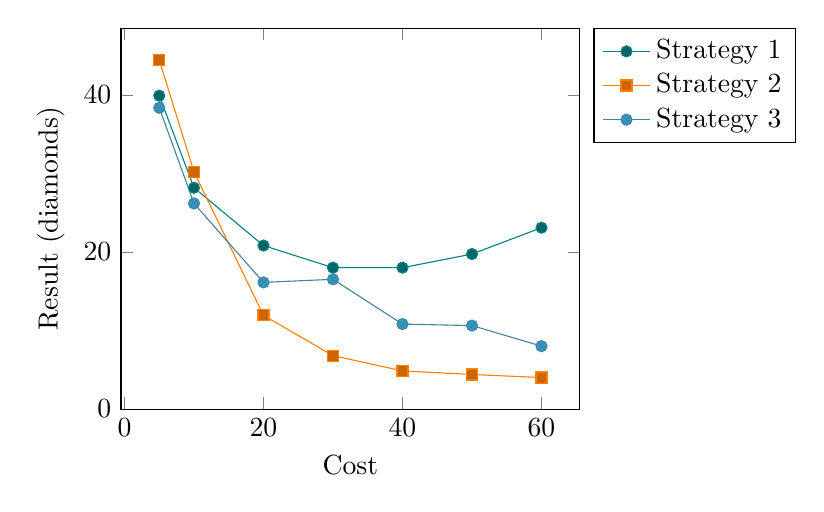
\begin{tikzpicture}
		\begin{axis}[
			xlabel = Cost,
			ylabel = Result (diamonds),
			cycle list name=exotic,
			legend pos=outer north east,
			scale=0.85
			]
			
			\addplot coordinates
			{(5,39.911633472184285)(10,28.184326096028368)(20,20.822328724414646)(30,18.002789090940414)(40,18.000106608201577)(50,19.737573735551326)(60,23.09285117463779)}
			;
			
			\addplot coordinates 
			{(5,44.4573499682562)(10,30.191633560819955)(20,11.927831753419248)(30,6.797546890999828)(40,4.854545454609092)(50,4.396643226971192)(60,4.009090909181819)}
			;
			
			\addplot coordinates
			{(5,38.36786030197544)(10,26.183473563067537)(20,16.128919602652935)(30,16.52013067842722)(40,10.818181821233052)(50,10.627417023079374)(60,8.009090909090908)}
			;
			
			\legend{Strategy 1, Strategy 2, Strategy 3}
			
			
		\end{axis}
	\end{tikzpicture}
	\caption{  }	
	\label{fig:result_adaptive_random_high_dim}
\end{figure}

\begin{itemize}
	\item compare all 5 techniques
\end{itemize}


\section{Comparison and Discussion}







